\documentclass[12pt]{article}

% TEMPLATE DEFAULT PACKAGES
\usepackage{amssymb,amsmath,amsfonts,eurosym,geometry,ulem,graphicx,color,setspace,sectsty,comment,natbib,pdflscape,array,adjustbox}

% ADDED PACKAGES FOR THIS MANUSCRIPT
\usepackage{palatino,newtxmath,multirow,titlesec,threeparttable,tabu,booktabs,titlesec,threeparttable,mathtools,bm,bbm,subcaption,pdflscape,tcolorbox,mathrsfs,tikz,float}
% endfloat,
% \usepackage[capposition=top]{floatrow}
\usepackage{tikzpagenodes}
\usepackage{pbox}

\usepackage{afterpage}
\usepackage[hyphens]{url}
\usepackage[margin=1cm]{caption}

\usepackage[draft]{hyperref}
\newcommand{\tim}{$\,\times\,$}
% FIGURES & TABLES CAPTION STYLING
\captionsetup[figure]{labelfont={bf},name={Figure},labelsep=period}
\captionsetup[table]{labelfont={bf},name={Table},labelsep=period}

% SECTION TITLE SETTINGS
\titlelabel{\thetitle.\enskip}
\titleformat*{\section}{\large\bfseries}
\titleformat*{\subsection}{\normalsize\bfseries}

% COLUMN TYPES
\newcolumntype{L}[1]{>{\raggedright\let\newline\\\arraybackslash\hspace{0pt}}m{#1}}
\newcolumntype{C}{>{\centering\arraybackslash}p{5.2em}}
\newcolumntype{D}{>{\centering\arraybackslash}p{5em}}
\newcolumntype{G}{>{\centering\arraybackslash}p{6em}}
\newcolumntype{R}[1]{>{\raggedleft\let\newline\\\arraybackslash\hspace{0pt}}m{#1}}


% MARGINS AND SPACING
\normalem
\geometry{left=1.1in,right=1.1in,top=1.0in,bottom=1.0in}
\setlength{\parskip}{2.5pt}

% SPECIAL CELL 
\newcommand{\specialcell}[2][c]{%
	\begin{tabular}[#1]{@{}l@{}}#2\end{tabular}}

% NO INDENT ON FOOTNOTES
\usepackage[hang,flushmargin]{footmisc}




\begin{document}

\begin{titlepage} 
\title{{Public Housing Spillovers in a Developing Country}\thanks{We are grateful to Andrew Foster, Daniel Bjorkegren, Matthew Turner, Jesse Shapiro, Brian Knight, and John Friedman for their feedback and advice.  We also thank Adelaide Steedley and the Centre for Affordable Housing and Finance in Africa as well as GeoTerraImage for generous research guidance and for providing data without which this project would not have been possible.  Any opinions and conclusions expressed herein are those of the authors and do not necessarily represent the views of the Federal Trade Commission or its Commissioners.}}
\author{\\[3em] Benjamin Bradlow\thanks{Dept. of Sociology, Brown University, Providence, RI  E-mail: benjamin\textunderscore bradlow@brown.edu}\\
 Stefano Polloni\thanks{Mapdwell, Cambridge, MA.  E-mail: stefano\textunderscore polloni@alumni.brown.edu}\\ 
  William Violette\thanks{Federal Trade Commission, Washington, DC. E-mail: william.j.violette@gmail.com} \\
 \\ 
  }
% \vspace{30mm}
\date{\vspace{5mm}This Version: \today}
\maketitle
\begin{abstract}

%%% STATEMENT HERE!  

	%Does subsidized housing improve neighborhood quality in developing countries? 

	% Public housing projects may complement local housing investments as well as substitute for existing housing, especially low-quality slums.  

	We estimate the direct and spillover effects of large public housing projects in South Africa using aerial measures of housing density, property transaction records, and census data.  We compare (1) constructed projects versus planned but unconstructed projects, (2) before versus after scheduled construction, and (3) areas nearby versus further from project footprints.  Projects increase the quantity and quality of formal housing within their footprints.  Between 0 and 500 meters outside of their footprints, projects generate declines in informal housing quantity and formal housing prices.  Estimates from a structural model of housing markets suggest that projects may result in welfare losses.

	% \footnote{We may want to establish the general question, object of study. Something like: “While public housing projects are generally assumed to improve welfare by virtue of providing improved housing conditions, we find wide variation in how such programs impact contemporary slum development in rapidly urbanizing contexts.}

%%%%%% MACRO THE HETEROGENEITY DISTANCE
%Within project footprints, housing quality improves and subsidized formal structures successfully crowd-out slums. 


\vspace{.1in}
\textbf{Keywords:} housing policy; place-based policy; urban development.\\
% \vspace{0in}\\
\textbf{JEL Codes:} O18; O22; H4; R3.  \\
\bigskip
\end{abstract}
\setcounter{page}{0}
\thispagestyle{empty}
\end{titlepage}
% \pagebreak \newpage

\spacing{1.4}
\section{Introduction} \label{sec:introduction}


% effects on slum growth as well as growth in 
% welfare effects depending on how local informal housing markets.  Place-based policies may distort local housing markets   Housing markets in developing countries may be especially responsive since they are informal
% represent an especially effective policy tool in developing countries because dense externalities are way stronger

% By providing new formal houses and improved infrastructure, housing projects may generate positive neighborhood amenities.  Projects may also have unintended consequences by attracting growth of low-quality, informal dwellings in the backyards of project houses \citep{Brueckner2018backyarding}.  Dense backyard dwellings may recreate slum conditions and depress neighborhood property investment.  The net spillover effects of housing projects remain an empirical question that has important implications for designing place-based policies that address slum growth.

% Local housing markets are very elastic so place-based policies may not succeed at redistribution?
% Unlike standard poverty reduction policies that target households, place-based policies promote development in specific areas. 
% Since slum conditions discourage local investment, slums often persist in 

%  inexpensive land.  Many cities target slums with place-based policies including land-titling, in-situ upgrading, and public housing.  Unlike standard poverty reduction policies that target households, place-based policies promote development in specific areas. 

% Launch into place-based policies

% The United Nations aims for countries to ``by 2030, ensure access for all to adequate, safe, affordable housing and upgrade slums.'' 



% These policies aim not only to improve housing quality, but also to spur investment in surrounding neighborhoods.  
% policymakers aim to reverse these conditions with place-based policies

% These policies aim not only to improve housing quality for existing slum-dwellers, but also to 
% , but also to spur investment in surrounding neighborhoods.  

%  with place-based policies  
% Since slum conditions discourage households from investing in these neighborhoods, slums often become dense clusters isolated from other neighborhoods.   

% Since many households prefer not to live next to slums, 
% As property developers avoid these areas
% these conditions make it less desirable to live next to
% Slum conditions often discourage investment in nearby housing quality.  
% , slums often grow dense, homogenous, and isolated from other neighborhoods.  

% Slums often cluster on pockets of inexpensive land
% weaken incentives
% Since these conditions weaken incentives to invest in these areas, slums grow to become dense, clusters

% concentrated, isolated, clustered
% rather than spread evenly across the city, slums are clustered...
% pockets
% why are they

% Slums often concentrate in areas with  and grow to become dense, homogenous areas..
% concentrate in specific neighborhoods 

% While slums are often clustered in specific neighborhoods, they may negatively affect surrounding neighborhoods as 

% In addition to poverty reduction programs, many cities target slums with spatially 



% While many cities lack the resources to target slum growth directly, some cities have responded by replacing slums with large public housing projects.  

% For example, the South African Department of Housing promotes ``accelerating the delivery of housing as a key strategy for poverty alleviation,'' while also ``utilizing housing as an instrument for the development of sustainable human settlements, in support of spatial restructuring'' \citep{bng}.  



% As a first goal, ``every municipality must... ensure that the inhabitants of its area of jurisdiction have access to adequate housing on a progressive basis.''\footnote{See \cite{housingact}.}  Our results provide evidence that housing projects boost the quantity and quality of dwellings available to households within project footprints.  Building density estimates find increases in formal housing with no changes in total informal housing, reinforcing census estimates that document improvements in infrastructure access and housing quality.

% As a second goal, ``government must use public money available for housing development in a manner which stimulates private investment in, and the contributions of individuals to, housing development.''\footnote{Ibid.}    We find little evidence that housing projects are able to attract local investment in housing markets within and outside of their footprints.  Instead, formal housing growth nearby remains unchanged while prices for formal houses drop especially in relatively higher income areas.

% Finally as a third goal, ``government must promote the establishment, development and maintenance of socially and economically viable communities and of safe and healthy living conditions to ensure the elimination and prevention of slums and slum conditions.''\footnote{Ibid.}  



% 30\% of urban populations in developing countries live in slums characterized by overcrowding, poor infrastructure access, and informal dwellings made of non-durable material \citep{mdg}.  In slums, low quality housing may lead to unsanitary, congested neighborhoods, which then discourage new housing investments \citep{marx2013slums}.  To break this cycle, cities target slums with place-based policies including land titling, slum upgrading, and subsidized public housing.  These policies aim not only to improve housing quality, but also to spur investment in surrounding neighborhoods.  For example, the South African Department of Housing promotes ``accelerating the delivery of housing as a key strategy for poverty alleviation,'' while also ``utilizing housing as an instrument for the development of sustainable human settlements'' \citep{bng}.  Across Africa, governments have constructed over 5.4 million subsidized houses since 1994 ranging from 2,500 in Benin to 3 million in South Africa.

% 30\% of urban populations in developing countries live in slums characterized by overcrowding, poor infrastructure, and informal dwellings made of non-durable material \citep{mdg}.  Crowded, low-quality houses may lead to congested infrastructure and unsanitary conditions, which then discourage new housing investments \citep{marx2013slums}.  To break this cycle, cities target slums with place-based policies including land titling, slum upgrading, and subsidized public housing.  These policies aim not only to improve housing quality, but also to spur investment in surrounding neighborhoods.  For example, the South African Department of Housing promotes ``accelerating the delivery of housing as a key strategy for poverty alleviation,'' while also ``utilizing housing as an instrument for the development of sustainable human settlements'' \citep{bng}.  Across Africa, governments have constructed over 5.4 million subsidized houses since 1994 ranging from 2,500 in Benin to 3 million in South Africa.



% 30\% of urban populations in developing countries live in slums characterized by overcrowding and informal houses made of non-durable material \citep{mdg}.  Dense slums may produce congestion and unsanitary conditions, which discourage new housing and infrastructure investments \citep{marx2013slums}.  To break this cycle, cities target slums with place-based policies including land titling, slum upgrading, and subsidized public housing.  Across Africa, governments have constructed over 5.4 million subsidized houses since 1994 ranging from 2,500 in Benin to 3 million in South Africa.  These policies aim not only to improve housing quality, but also to spur investment in surrounding neighborhoods.  For example, the South African Department of Housing promotes ``accelerating the delivery of housing as a key strategy for poverty alleviation,'' while also ``utilizing housing as an instrument for the development of sustainable human settlements'' \citep{bng}.  


30\% of urban populations in developing countries live in slums characterized by overcrowding and informal houses made of non-durable material \citep{mdg}.  Dense slums often produce congestion and unsanitary conditions, which discourage new housing and infrastructure investments \citep{marx2013slums}.  To break this cycle, cities target slums with place-based policies including land titling, slum upgrading, and subsidized public housing.  Across Africa, governments have constructed over 5.4 million houses from 2,500 in Benin to 3 million in South Africa \citep{bah2018housing}.  
% These policies aim not only to improve housing quality, but also to spur investment in surrounding neighborhoods.  For example, the South African Department of Housing promotes ``accelerating the delivery of housing as a key strategy for poverty alleviation,'' while also ``utilizing housing as an instrument for the development of sustainable human settlements'' \citep{bng}.  

% These additional investments may amplify any direct welfare gains to the recipients.  
Place-based policies can have ambiguous welfare effects depending on how they interact with local housing markets.  When policies improve neighborhood amenities like housing quality or infrastructure, nearby households may also invest in the quality of their homes.  Developers can capitalize on these amenities by building new, local houses.  Place-based policies also risk distorting property markets.  For example, public housing projects may replace private housing investment that may better accommodate local housing needs.  

In developing cities, slums may amplify the welfare effects of place-based policies.  Policies that upgrade slums yield additional benefits by reducing congestion, improving sanitation, and inviting infrastructure investment.  Policies can also have unintended consequences by attracting new slum growth.  For example, public housing projects may leave room for households to build low-quality houses in the backyards of project houses \citep{Brueckner2018backyarding}.  Dense backyard housing may recreate slum conditions and depress neighborhood property investment.  The net effects of these policies remain an empirical question that has implications for designing place-based policies in developing cities.



% In developing cities, informal housing markets 
% In developing cities, the presence of slums may exacerbate the welfare effects of place-based policies.  Positive effects 



% Developing cities feature elastic, informal housing markets, which may exacerbate 

% For example, public housing projects may represent positive neighborhood amenities, driving nearby households to invest in their homes.  Developers may capitalize on these amenities by building new, high-quality homes.  At the same time,

% invite nearby households to invest in their homes.  

% - in for the long haul, investing in their houses, 


% For example, new houses 

% new houses and infrastructure from public housing projects may invite nearby property investment as  

% For public housing projects, new houses and infrastructure may invite property investment nearby as 

%  that drive existing homeowners to upgrade their houses as well as new housing developments.

% Alternatively, public housing projects may improve the 

% analyzes the combined effects of eradicating existing slums and replacing them with housing projects

% which is unique among developing countries for its massive scale having allocated over 3 million houses across hundreds of projects since 1994.

%%%%  MOVE TO LITERATURE REVIEW !!!
% This large volume of projects allows us to identify spatial impacts, building on existing research which is largely limited to considering outcomes for direct project recipients.\footnote{\cite{cattaneo2009housing} estimate child health improvements from housing upgrades in Mexico, \cite{franklin2016enabled} finds greater women's employment for public housing recipients in South Africa, and \cite{galiani2017shelter} combine housing projects from throughout Latin America, finding large improvements in reported well-being of households.} 

% which builds two-room houses often replacing preexisting slums.  
% formal and informal houses
% To measure these impacts, we compile detailed spatial data for the Johannesburg metro-area including aerial measures of formal and informal houses, census data, as well as deeds records of formal housing transactions.  
% WHAT ARE THE PROBLEMS!! 


%  and within their surrounding neighborhoods
This paper analyzes the effects of public housing projects both within and nearby their footprints.  We focus on South African housing projects where the government acquires land, clears existing slums, and constructs hundreds of single-story, two-room houses.  We compile detailed spatial data for the Johannesburg metro-area including household census data, deeds records of formal housing transactions, and an aerial panel of all buildings.  The aerial panel provides a novel measure of slum growth by distinguishing between formal and informal houses according to building materials and appearance.  

%  This evidence suggests that governments may follow precise criteria in selecting plots for projects.  

Using spatial data, the standard approach to evaluating place-based policies may produce biased estimates in our setting.  The standard approach compares changes in outcomes nearby versus further away from projects under the assumption that these areas would have evolved in the same way in the absence of projects.\footnote{See \cite{diamond2016wants,rossi2010housing,hornbeck2017creative} for examples.}  In our setting, we document that projects are located not only in poorer neighborhoods, but also on specific plots of land with dense slums and few formal houses.  Dense slums may lead these plots to develop differently from neighboring plots even in the absence of project construction.

We propose comparing changes in outcomes for constructed projects to changes in outcomes for planned, but unconstructed projects.  Both constructed and unconstructed projects are located on similar types of plots within their neighborhoods.  Since projects are located in different types of neighborhoods, we also control for changes in outcomes across constructed and unconstructed project neighborhoods.  Our empirical strategy allows us to identify the causal effect of housing projects under the assumption that differences between project areas and their neighborhoods would have evolved in the same way between constructed and unconstructed projects in the absence of construction.

%  since constructed projects are more likely to be located in neighborhoods with dense housing, we also control for time trends .

% differences between these neighborhoods.  

% project construction is more likely in neighborhoods with more preexisting housing.

%   We face an additional challenge

% Since project construction is more likely in neighborhoods with more preexisting housing, we also control for changes in outcomes further away from projects in the same neighborhoods 

% to account for any  to account for the possibility of differential trends across neighborhoods.


% This approach requires the assumption that in the absence of project construction, both areas would evolve in a similar way.  
% Projects are located on appear to target plots within neighborhoods similarly across constructed and unconstructed projects.   since 

% In order to identify these effects, we leverage three comparisons:  First, we compare constructed projects versus planned but unconstructed projects to control for how governments strategically locate projects on undeveloped land with preexisting slums.  Second, we compare projects before versus after scheduled construction to control for how neighborhoods with constructed projects often have more preexisting housing than neighborhoods with unconstructed projects.  Third, we compare areas nearby versus far from a project footprint within the same neighborhood to control for housing market trends specific to each neighborhood.  

% Standard methods that compare changes in project areas 
% Standard methods that evaluate place-based policies by comparing changes in project areas to changes further away 

%  which presents a challenge for   Standard methods 
%  housing projects according to spatially precise criteria, which presents a challenge for identifying suitable counterfactual 
% on land plots with dense slums and few formal houses compared to neighboring plots within 100 meters.  This evidence suggests that , which presents a challenge for identifying 

% We document that constructed projects 
% evidence of governments locating projects on plots of land with dense slums and few formal houses.  
% We provide evidence of governments locating projects on plots of land with dense slums and

%   which presents a challenged for identifying counterfactual areas 

% Since governments locate housing projects carefully and intentionally, it can be difficult to identify the effects of housing projects instead of how these plots of land would have developed...
% we face challenges identifying
% can't be identified with standard approach because   the land is carefully chosen!
% housing projects are difficult to identify,,, housing 
% Since governments locate housing projects carefully and intentionally, it can be difficult to identify the effects of housing projects instead of how these plots of land would have developed...
% We document that housing projects are located on land with dense preexisting slums and little formal housing development.  


% Our main estimates combine these three comparisons into a triple-differences estimator, which extends standard difference-in-differences approaches by allowing for the endogenous placement of projects within neighborhoods.\footnote{See \cite{rossi2010housing,hornbeck2017creative}, and \cite{diamond2016wants} for difference-in-differences estimators of place-based policies.}  

We find that housing projects more than double the number of formal houses within their footprints, suggesting both that projects are  successful and that footprints do not experience large, private investments in housing in the absence of projects.  According to our estimates, projects have zero effect on the number of informal houses in their footprints.  While projects eradicate existing informal houses, they also invite substantial growth of backyard houses, which may partially undermine South Africa's goals to ``ensure the elimination and prevention of slums and slum conditions.''\footnote{See \cite{housingact}.}  Census results at the census block-level provide some evidence that projects improve access to infrastructure like piped water; however, noisy estimates reinforce the need for precise spatial data to evaluate place-based policies.  

For spillover areas between 0 and 500 meters from housing projects, we estimate declines in formal housing prices with no change in formal housing quantity.  We also estimate declines in the number of informal houses, which almost offset the increase in houses within project footprints.  These findings suggest that projects may create neighborhood disamenities, weakening incentives for local housing investment.  In this way, housing projects may fail to advance the government's goals ``to use money available for housing development in a manner which stimulates private investment in, and the contributions of individuals to housing development.''\footnote{Ibid.}

% For these housing markets, formal price changes and informal quantity changes are consistent with inelastic formal supply and elastic informal supply.  These results stress the importance of collecting housing quantity data to measure the welfare effects of place-based policies in developing countries. % put in a comparison to developed countries?

%%% UNIQUE TO HAVE THIS QUANTITY DATA!! 


To map changes in housing quantities into welfare estimates, we build an equilibrium model of housing markets where projects affect the amenity value of living both within project footprints as well as 0 to 500 meters away from footprints.  In the model, developers choose to build houses on land plots when the value to households from renting and enjoying local amenities exceeds the construction costs.  Variation in construction costs allows us to estimate household demand for housing and express amenity values in monetary terms.  We construct a spatial measure of construction costs according to land steepness.  By focusing on housing quantities, our model may have useful applications for place-based policies in other developing contexts because price data are often scarce while housing quantity measures are increasingly available through remote sensing.\footnote{ \cite{marxthere} use satellite images to measure density and improvements in the quality of roofs in a Kenyan slum.  \cite{Brueckner2018backyarding} use the same satellite data as this paper to study backyard houses in South Africa. \cite{donaldson2016view} review several research projects using building-level remote sensing data to map urban growth especially in developing countries. }  

% The model does not explicitly account for externalities 
% use variation in construction costs from land elevation to 
% that maps housing density effects into household preferences for living within and nearby housing projects.  
% Housing projects may affect both local construction costs as well as the quality of local amenities.  

Structural estimates suggest that housing projects are likely to reduce aggregate welfare.  By subsidizing home construction, projects generate welfare gains for formal housing markets within their footprints; however, these gains are overwhelmed by the costs of project implementation as well as negative spillover effects on nearby formal and informal housing markets.  According to the model, projects result in a total welfare decline of 3 billion USD (ranging from -11.3 to 5.3 billion USD at 95\% confidence), which includes total implementation costs of 558 million USD.\footnote{Implementation costs are derived from the National Treasury's Annual Budget Reports.} 


% simulation exercises permit a wide range of welfare effects averaging 2.4 billion USD with a 

% suggest economically large welfare losses on the order of 6.6 million USD per project (including implementation costs of 3.2 million USD per project).

% [ LITERATURE REVIEW ( AGAIN ) ]
% Since this framework assumes that land owners are able to capture all rental surplus, the distributional consequences of these policies depend on which households are also land owners.  Without data on ownership over time especially for informal housing, we instead explore distributional consequences by examining effects separately by neighborhood income quartile.
%% give credit to simon franklin for planned-but-unconstructed strategy
% These studies find largely positive effects:  \cite{rossi2010housing} 

 
This paper contributes to growing research on place-based policies.  Studies in the US compare changes in outcomes either (1) near versus far from project areas\footnote{See \cite{rossi2010housing,hornbeck2017creative}, and \cite{diamond2016wants}.} or (2) in constructed versus planned, but unconstructed project areas.\footnote{See \cite{busso2013assessing} and \cite{kline2013local}.}  Most closely related to our work, \cite{diamond2016wants} find that public housing projects in the US increase housing prices in low-income neighborhoods and decrease housing prices in high-income neighborhoods.  

In developing countries, researchers often lack panel data and instead, rely on cross-sectional comparisons producing mixed results.  In Tanzania, \cite{baruah2017planning} observe that areas near sites-and-services programs have better housing quality than similar, untreated areas.  Using a similar design in Jakarta, Indonesia, \cite{harari2018slum} find declines in local land values and levels of formalization.  \cite{gechter2018slums} link changes in Mumbai's zoning laws to formal housing development and higher nearby property prices.  Our study contributes to this literature by using spatial panel data and unconstructed project counterfactuals to examine a large-scale place-based policy.
 % examining a place-based policy in South Africa with identification strategies from 

Our study also relates to recent research on South Africa's national housing program focusing on outcomes for direct beneficiaries of project houses.  Using household surveys, studies estimate the effect of receiving a project house on women's labor supply: \cite{picarelli2019there}  finds negative effects nationally while \cite{franklin2016enabled} finds positive effects in Capetown.  \cite{franklin2016enabled} also shows that planned, but unconstructed projects may provide useful counterfactuals to estimate project effects in this context.

% \cite{franklin2016enabled} 
% We also contribute to research on housing projects in South Africa ;  cite natalie and simon ;  say we fill the gap by looking locally
% Finally, outside of the developing world, our research draws upon an established literature on housing externalities \citep{rossi2010housing,hornbeck2017creative,diamond2016wants}. 

We proceed by first providing background on public housing and the South African national housing program in Section~\ref{section:background}.  Section~\ref{section:data} describes the data used to measure outcomes and details our approach to identifying housing projects. Motivated with descriptive evidence in section~\ref{section:descriptives}, Section~\ref{section:methodology} lays out the estimation strategy and identifying assumptions. Section~\ref{section:results} presents our main results.  In Section~\ref{section:theory}, we build an equilibrium model of housing markets and estimate welfare effects.   Section~\ref{section:discussion} concludes.




\section{Public Housing Projects}\label{section:background}


European cities began investing in social housing programs in the early 20th century, and national governments in the West continued to grow these investments in the post-WWII era. After the wave of de-colonization in the 1950s, many developing nations also began public investments in housing, which were progressively phased out in order to secure international financing for national debt crises in the 1970s and 1980s \citep{rondinelli1990housing}. Beginning in the 1990s large middle-income countries took on subsidized housing programs that focused on channeling public funds to private developers to build full top-structure dwellings. Chile, South Africa, and Brazil are examples of this more recent approach \citep{buckley2005housing}.


\subsection{Public Housing in South Africa}


The housing projects studied in this paper were implemented as part of a large national housing scheme enacted in 1994. Though periodically revised and renamed,\footnote{Public housing in South Africa has been delivered under the {\it Reconstruction and Development Program} (RDP) starting in 1994 and  by its successor, {\it Breaking New Grounds}, as of 2004.} the program has consistently sought to redress the economic and geographic legacy of apartheid by providing formal housing to low-income households.  

This program allocates yearly funds to local housing authorities to construct and allocate 40m$^2$, single-story, two-room houses on individual plots.\footnote{Local housing authorities include provincial housing departments and municipal housing departments for urban areas like Johannesburg \citep{dhsreports}.}  Local authorities identify large parcels of land that are able to each accommodate several hundred houses.\footnote{We draw on qualitative field work conducted over 7 months between 2015 and 2018, including interviews with City of Johannesburg and Gauteng provincial housing officials, to corroborate our understanding of the practical specifics of policy design and implementation.}  To meet budgetary targets, authorities often identify inexpensive land located on the urban periphery.\footnote{See Interview with author, 23 August 2017 and \cite{dhsreports}}  In many cases, authorities combine housing projects with slum eradication goals by replacing preexisting informal settlements with new housing projects \citep{hofmeyr2008risk}.  Since project construction requires passing an environmental impact assessment, receiving zoning approval from local municipalities, and providing infrastructure access, authorities implement the most feasible subset of candidate projects each year.\footnote{Existing policy research characterizes South African housing as an opaque, top-down system where government authorities locate and allocate houses with minimal participation from local communities \citep{seriq}.  Tissington [2012] documents how local community calls for housing improvements in Guateng were left unanswered for over a decade by local authorities.  \cite{seriq} report how the Gauteng government refused to provide information about plans for housing subsidies and allocation to the Soweto Form, a local community based organization (p. 67).}   Housing authorities subcontract with local housing developers for housing construction.  According to government figures, upwards of 3 million housing units have been delivered nationally between 1994 and 2015.


Eligible households are required to sign up for an official waiting list maintained by the National Department of Housing.\footnote{According to the General Household Surveys, 2009 to 2013, the share of households reporting at least one member on the waiting list has remained stable at over 13\% from 2009 to 2013.}  Eligibility requires South African citizenship, no previous property ownership, being married or having financial dependents, and having a monthly household income below R3,500 \citep{seriq}.  Each project house is assigned to a beneficiary in a first-come, first-served basis according to the beneficiary's place in the waiting list for the province or municipality. When projects replace existing informal settlements, previous inhabitants have priority for receiving project houses.  Beneficiaries are expected to pay a small one-time payment in order to receive title for their houses.  Guidelines also prevent beneficiaries from reselling their houses within their first 7 years of ownership.   %\footnote{The Gauteng Province has implemented their own waiting list since 2008 in order to exert greater control over the allocation process.}

In practice, these guidelines are loosely followed.  Recent reports point to cases of corruption in the allocation of houses \citep{seriq}.\footnote{Research suggests that beneficiaries are often selected over the course of project construction and sometimes even after construction has finished \citep{seriq}.}  Also, more than 15\% of project houses are reported as being still occupied by their original beneficiaries within five years of construction.\footnote{This figure is calculated from the General Household Surveys from 2009 to 2013. Anecdotal evidence suggests that project managers are aware of active secondary markets but have difficulty policing these transactions \citep{resale}.} 


% \subsubsection{Backyard Shacks}

% By design, subsidized housing in South Africa offers recipients [[[[ generous amounts of yard space ]]]], often diverted to alternative land uses. The construction of informal backyard shacks is a common occurrence within project boundaries. Recipients typically enter agreements with tenants (at times relatives) to lease the shacks for cash or in-kind payments. According to the 2011 census, backyard tenants represent 7.5\% of South African households.\footnote{This figure jumps to 12.5\% for the province of Gauteng, where our study is conducted.} Though the structures are not as durable as their government-provisioned counterparts, living conditions are typically superior to conventional informal settlements. Tenants gain indirect access to their landlord's services such as water taps, electricity connections, and toilets, and benefit from reduced eviction threats and greater personal safety \citep{beall2003social}. \cite{Brueckner2018backyarding} note that {\it backyarding} is suggestive of inefficiencies in the program delivery, and allows households to correct potential misallocations of resources. Importantly for our analysis, backyard shacks reveal that more households may benefit from subsidized housing than the listed number of direct recipients. According to the General Household Surveys (2009-2013), more than 33\% of government-provisioned homes have backyard shacks within two years of the delivery date. 


% \subsection{Estimating Housing Demand}


% The triple-difference approach also provides a useful framework for estimating residential housing demand given by equation (\ref{eq:housingdemand}).  Our empirical setting allows us to identify the causal effect of housing projects on local amenities net of unobserved housing costs.  Variation in housing costs also identify the marginal utility of income, which helps translate amenity effects of housing projects into monetary welfare estimates.




\section{Data}\label{section:data}

% Our analysis focuses on the South African province of Gauteng, both the smallest geographically and most populated province in the country. Gauteng's boundaries roughly correspond to the greater metropolitan areas of Johannesburg and Pretoria. 

Understanding the local impacts of public housing requires a precise measure of the location, timing, and size of housing projects complemented by outcomes at high spatial resolutions.

We locate projects using a map of housing projects obtained from the Gauteng City Regional Observatory, a research unit composed of the Gauteng Provincial Government and two Johanesburg universities.\footnote{\href{url}{www.gcro.ac.za/}}  The map describes 642housing projects as of 2008, including notes on their completion status.  We classify 172projects with descriptions including ``current,'' ``under implementation,'' or ``complete'' as constructed projects.  We then classify 145projects with descriptions including ``proposed,'' ``under planning,'' ``future,'' ``investigating,'' and ``uncertain'' as planned but unconstructed projects.  The remaining 325projects either do not include descriptions or their descriptions are difficult to classify as either constructed or unconstructed.  Appendix Table~\ref{table:projectdescriptions} includes tabulations of the full list of descriptions.  To supplement our understanding of project implementation, we conducted qualitative fieldwork over 7 months between 2015 and 2018, including interviews with housing officials in the municipal government of Johannesburg and provincial government of Gauteng. 

%Unclassified projects are more likely to be located in the northern region of the Gauteng province according to the map in Figure~\ref{figure:map}, which suggests that housing authorities in northern areas like Pretoria area may have followed different record keeping practices compared to those in the Johannesburg metro area.  
% 87of the unclassified projects are described as ``informal,'' which may correspond to government efforts to identify informal settlements rather than.

% Additional information for some projects allows us to examine the impacts of different types of housing projects.  We identify 56in-situ upgrading projects as those with descriptions containing the phrase ``Essential Services,'' which are linked to an aggressive demolition and rebuilding campaign launched by the Gauteng Province between 2000 and 2008 (\cite{hofmeyr2008risk}).  Likewise, we identify 63greenfield projects as those with descriptions containing the phrase ``Mixed Housing Developments,'' which were designed to modernize greenfield projects by combining project houses with investments in local services (\cite{greenfield}).

For constructed projects, we assign a completion date to each project according to the date when recipients received deeds to their project houses.  To recover this date, we overlay project locations onto deeds data from the South African National Deeds Office.  The deeds cover the universe of housing transactions from 2001 to 2011 in ``affordable areas,'' which are defined as census enumeration areas with 2010 mean house prices below R500,000.\footnote{These data were provided by the Affordable Land and Housing Data Centre, which tracks affordable housing markets.} Deeds include price, GPS location, plot size, buyer name, and seller name.  Although the data do not identify whether deeds belong to housing projects, we are able to infer project status according to whether the seller name includes a government or municipality when first transacted.  This project definition also excludes deeds flagged as large buildings used for commercial purposes (less than 2\% of transactions) as well as purchase prices more than R50,000 above the yearly nominal subsidy values (less than 4\% of remaining transactions), resulting in a sample of over 48,000 deeds.  Appendix Figure \ref{figure:transactionhist} plots the histogram of sale prices according to this project definition, finding substantial bunching around subsidy values for project deeds and a smooth distribution for non-project deeds.  We assign a completion date according to the modal year and month for deeds within each project.  Within projects, most government-sponsored properties are transacted in the same month.\footnote{Appendix \ref{appendix:histfreq} plots the distribution of subsidized and non-subsidized transactions around the modal transaction month.} 

For planned but unconstructed projects, we approximate expected completion dates by matching project names to National Treasury budget reports, which list expected project completion dates.  We digitized data for 422projects from budget reports spanning 2004 to 2009, which detail the name, start date, expected completion date, and cost of each housing project.  We then use a string-matching algorithm to link project names from the budget reports to the administrative maps.  Out of the 642 total project names from the administrative map, we are able to match 322 projects, including 126 constructed projects and 73 planned but unconstructed projects.  We provide further details about the digitization and string-matching algorithm in Appendix~\ref{appendix:stringmatch}.  Because of the low rate of matches, we use expected completion dates only for a subsection of the empirical analysis that focuses on estimating the immediate price impacts of housing projects.  The majority of the analysis compares outcomes in 2001 and 2011/2012 for constructed projects and for unconstructed projects under the assumption that these projects either were constructed or would have been constructed between 2001 and 2011/2012.

%%% MORE DISCUSSION OF THIS LIMITATION?

\begin{figure}[t!]
\centering
\caption{Housing Project Map}\label{figure:map}
% \tcbox[colback=white,boxrule=.35mm,boxsep=0mm]{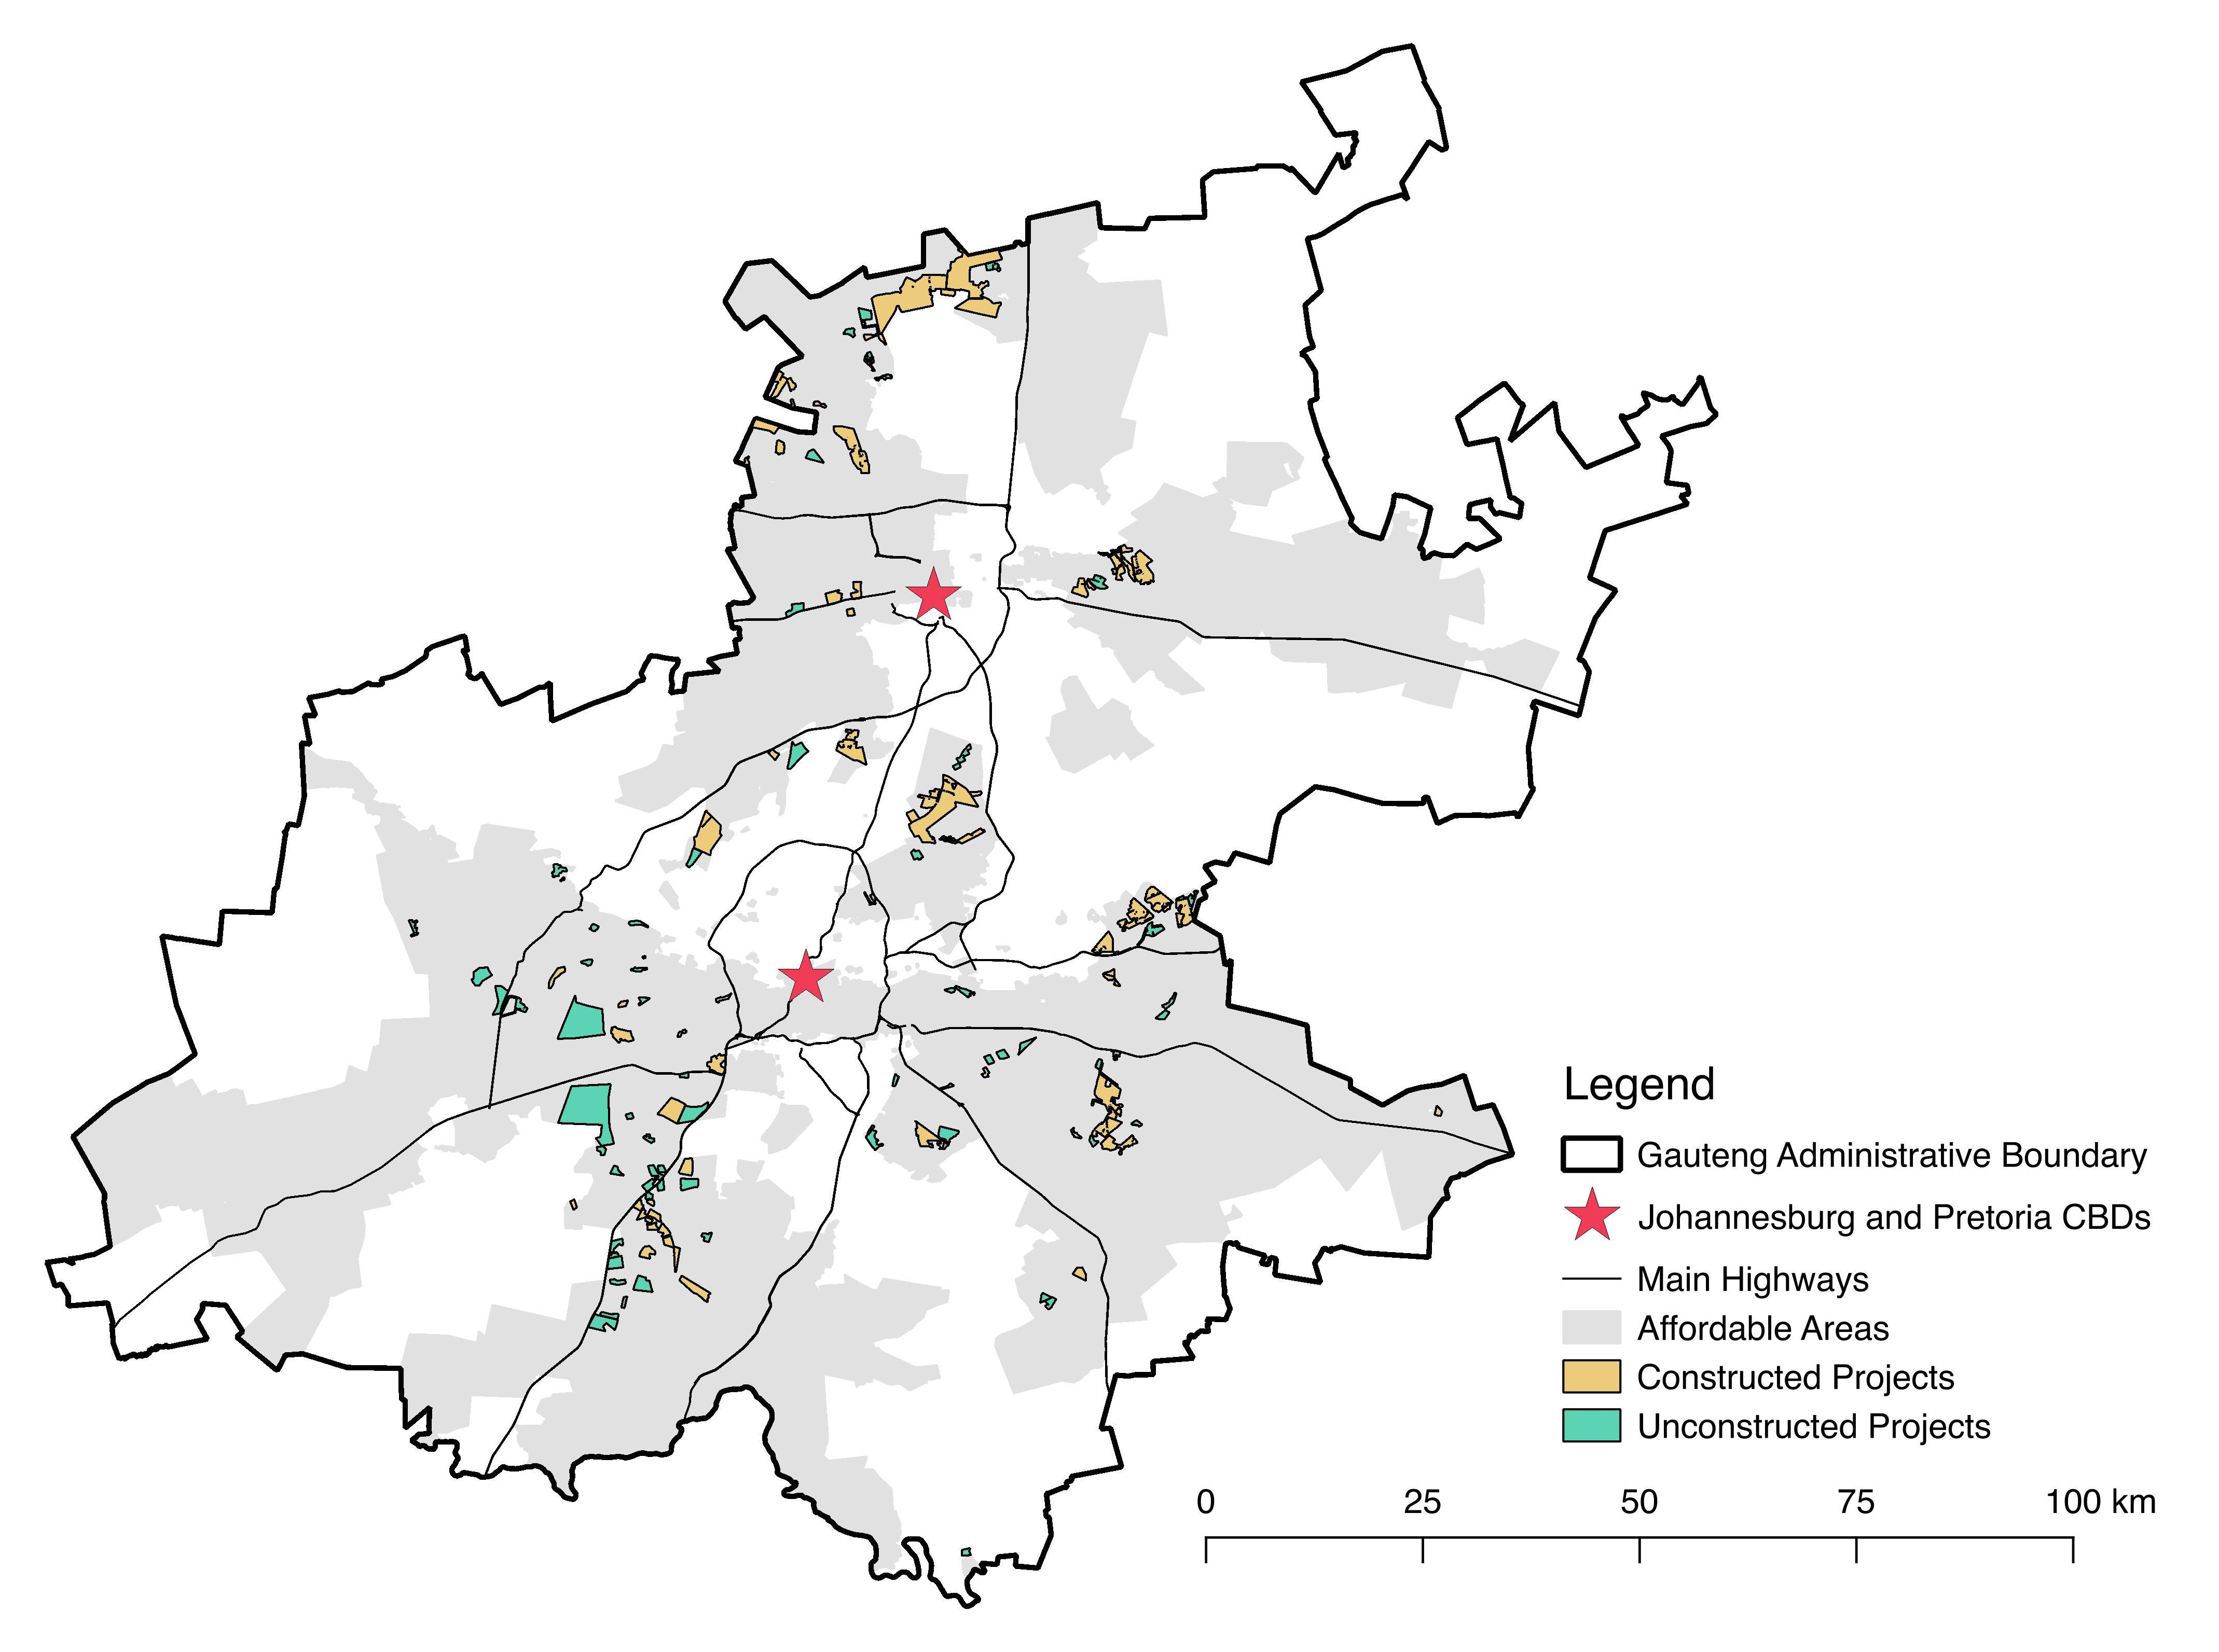
\includegraphics[scale=.098,trim={.9cm .4cm .9cm .4cm}]{figures/explanmap.jpg}}
% \tcbox[colback=white,boxrule=.35mm,boxsep=0mm]{\includegraphics[scale=.6,trim={.9cm .4cm .9cm .4cm}]{figures/newprojectmap.pdf}}
\tcbox[colback=white,boxrule=.35mm,boxsep=0mm]{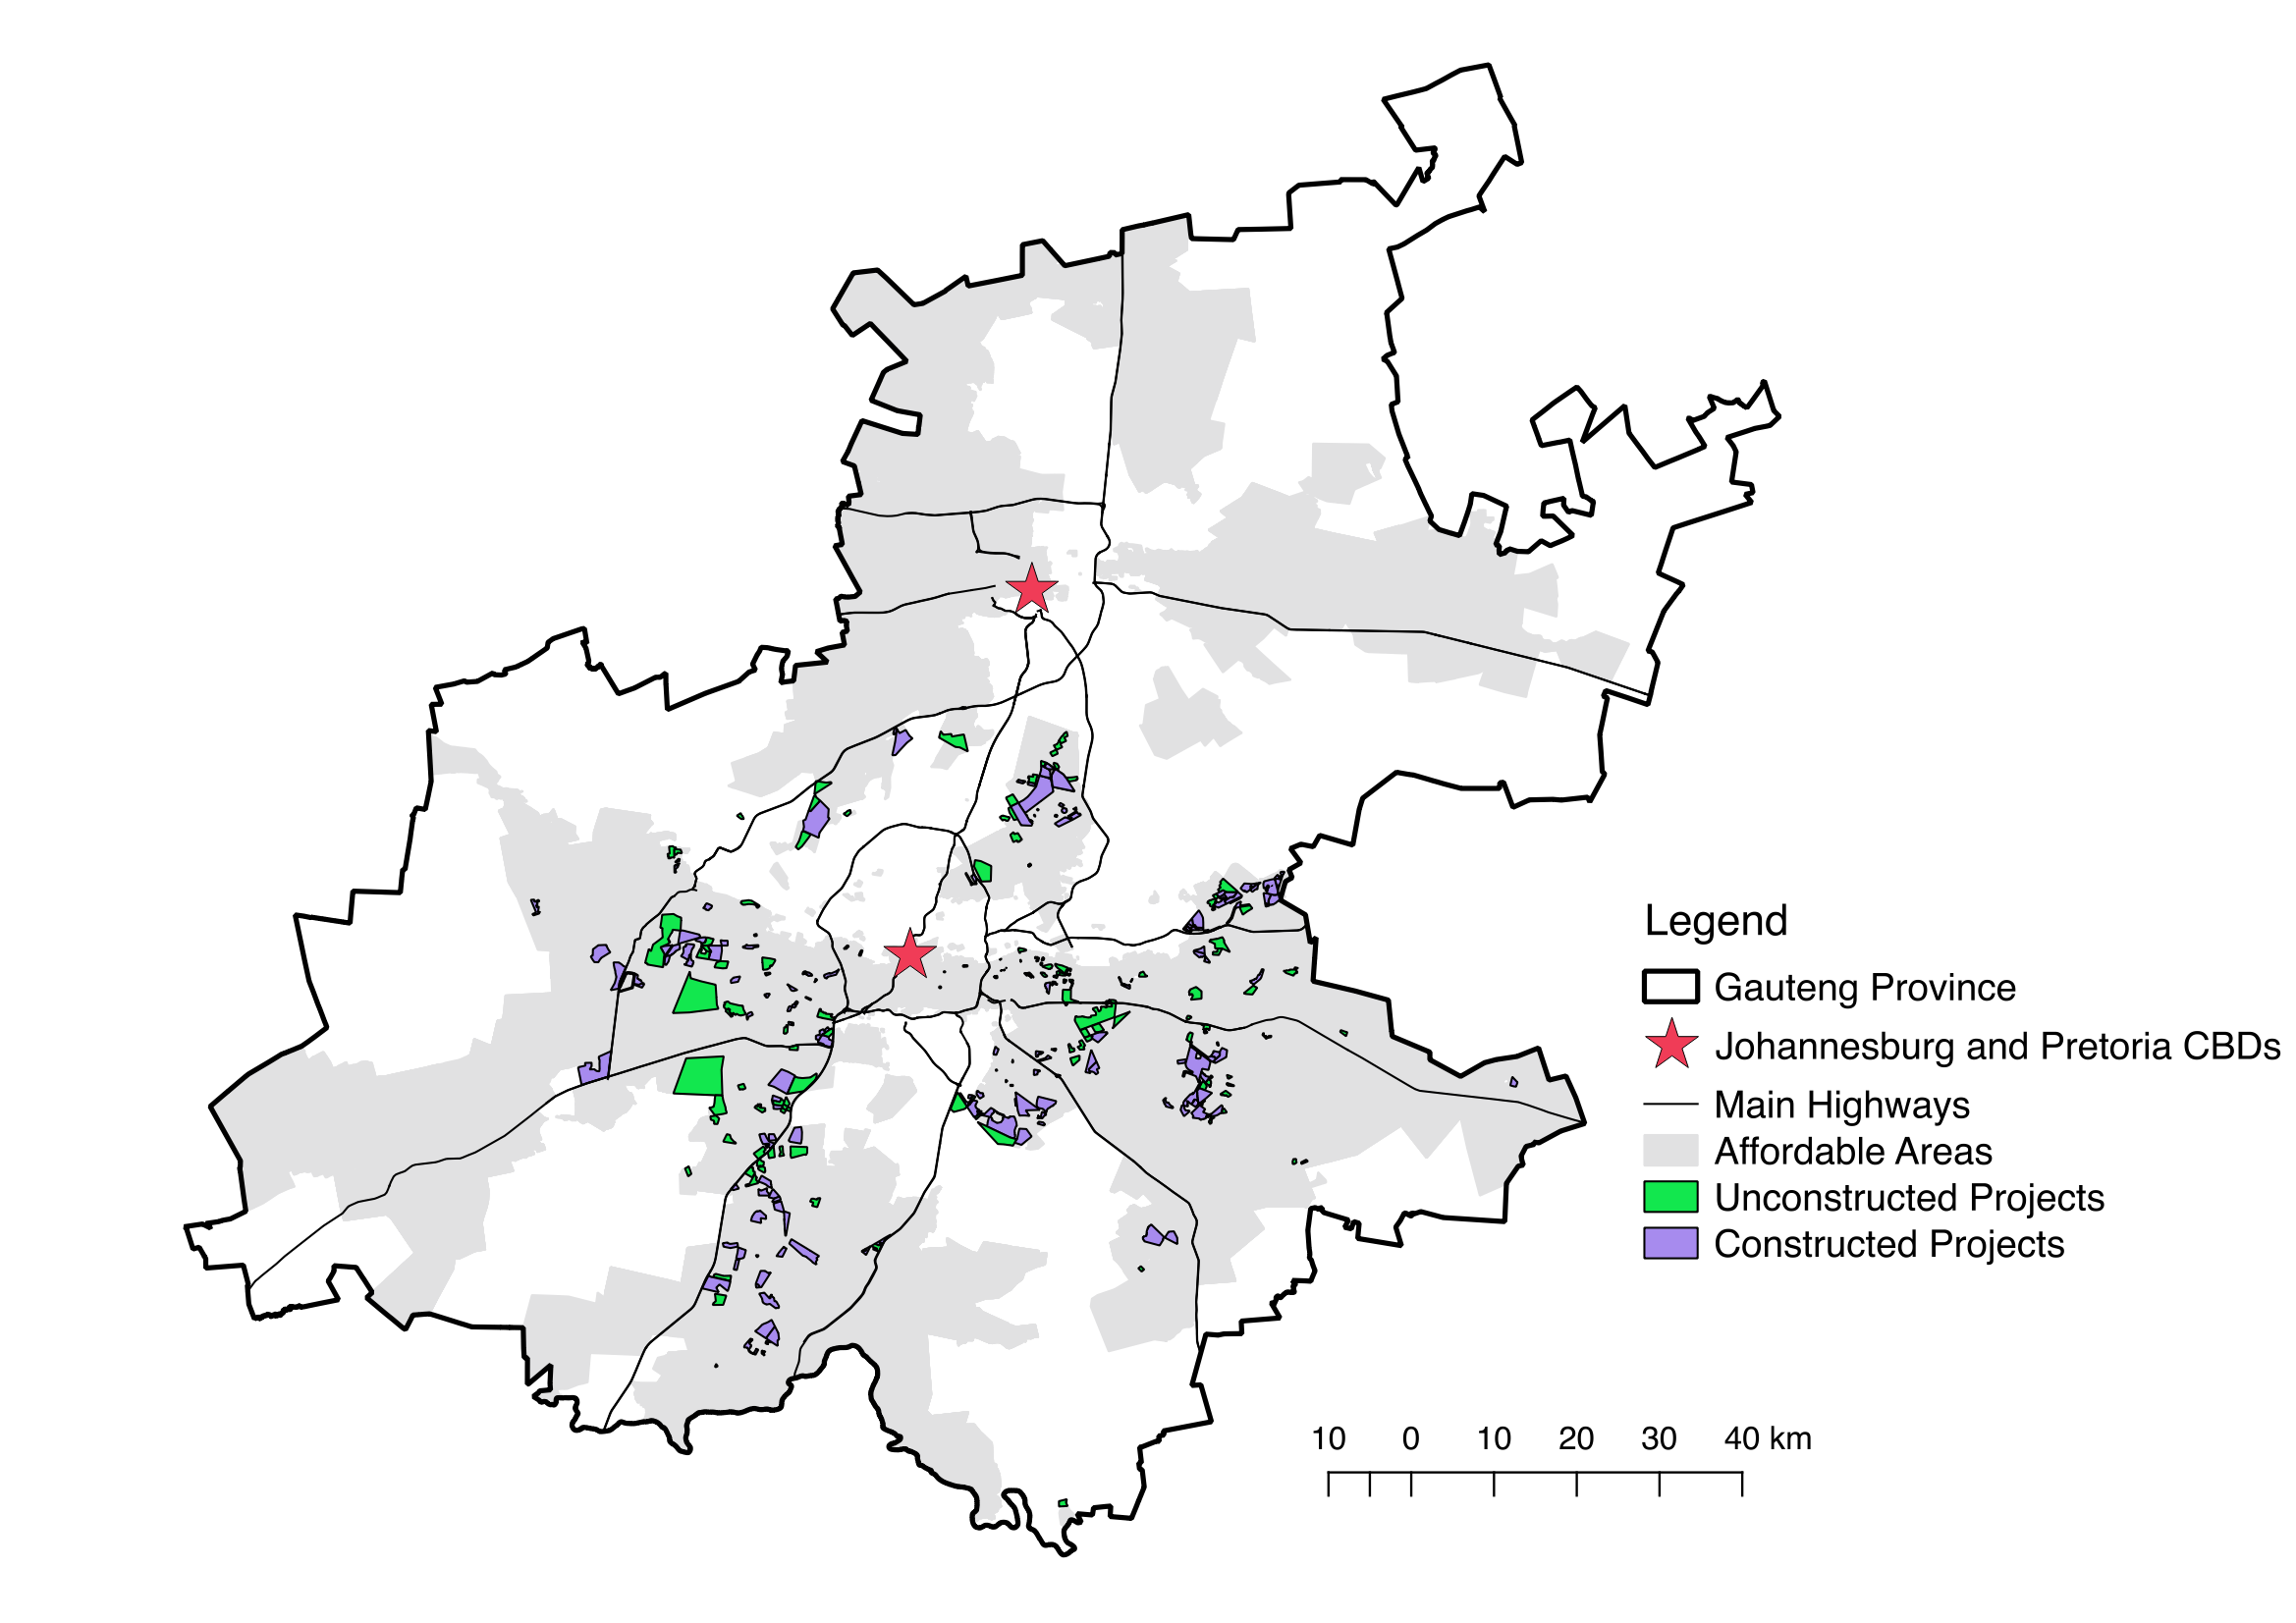
\includegraphics[scale=.6,trim={.9cm .4cm .9cm .4cm}]{figures/projmap_1.png}}
\end{figure}

Figure \ref{figure:map} maps the sample of constructed and unconstructed projects within the Gauteng province.  Projects are generally located far from central business districts, suggesting that inexpensive land plots are targeted by housing authorities.  Outside of the central business district, projects are distributed evenly throughout the Johannesburg metro area.  Despite their distance from the CBDs, projects are often next to arterial highways, potentially easing commuting costs for recipients.  We observe some constructed and unconstructed projects adjacent to each other while many other projects remain isolated.  Affordable areas -- the coverage area for our deeds data -- contain nearly every project boundary.  



%   Since project construction often occurs in phases, 
%  which is consistent with revisions in project planning and 

% Since project construction often occurs in phases, adjacent constructed and unconstructed projects may indicate partial project completion.  In many other cases, constructed and unconstructed projects are isolated from each other.

% In some cases, constructed and unconstructed projects are adjacent to each other, possibly indicating authorities were unable to complete different phases of planned projects, In other cases, isolated projects of both types.  



% We note that our approach is not without limitations, and may introduce measurement error insofar as we are misattributing deeds to housing projects (false-positives), or assuming a project is unconstructed when it was actually constructed (false-negatives).  

% To provide some validation for our classification, we tabulate in Table~\ref{table:projectdescriptions} project descriptions from the 2008 administrative policy maps according to whether projects are classified as constructed or unconstructed by 2011.  As of 2008, we find that constructed projects are more likely to be classified as ``completed" or ``under implementation", while unconstructed projects are more likely to fall into ``proposed'' or ``planning'' categories.  Among constructed projects, we find 5 ``proposed'' and 8 ``planning'' indicators, which could imply either (1) these projects are false-positives or (2) while planned at some point prior to 2008, these projects were eventually completed by 2011.\footnote{We are unable to assess the frequency at which these descriptions are updated in the data.}  We also identify a single ``complete'' project as unconstructed, likely because its houses do not appear in our deeds records.  Figure \ref{fig:forchange} in section \ref{section:descriptives} further validates our sample, showing how formal housing increases disproportionately in projects classified as constructed. 




% \subsection{Nearby housing transactions}


According to the 1997 Housing Act, the South African Government defines adequate ``housing development'' as (1) ``permanent residential structures with secure tenure, ensuring internal and external privacy and providing adequate protection against the elements'' and (2) ``potable water, adequate sanitary facilities and domestic energy supply'' (\cite{housingact}).  

First, to measure the number and quality of houses, we analyze hand-coded building data from 2001 and 2012 derived from high-resolution aerial and satellite imagery. We obtain these data from GeoTerraImage (Pty) ltd., a local remote-sensing specialist.\footnote{\href{http://www.geoterraimage.com/}{\tt http://www.geoterraimage.com/}} The data differentiate structures across 30 categories, including formal and informal residential houses. Informal houses are easily identified from their temporary nature, often made of materials such as recycled wood and corrugated metal. In contrast, formal houses are permanent, generally made out of brick and may have a pitched or a flat roof with tiles, zinc panels, or other materials. The data also distinguish between backyard houses and other types of informal houses.  As a validation exercise, we find high correlations ($\geq$0.85) between formal and informal house counts between this data and census data from 2001 and 2011.  To measure building density, we transform this data into 25m by 25m plot aggregates, creating five measures of housing density: (1) total residential structures split between (2) formal residential structures and (3) informal residential structures, which can be further decomposed into (4) backyard informal and (5) non-backyard informal structures.  We exclude plots where development is infeasible because the plots intersect with rivers, lakes, recreational locations (tennis courts, pools, basketball courts, etc.), and mining excavation areas (10\% of total plots).  
% In Figure \ref{fig:bblumaps}, we provide an example of the raw data and a depiction of our griding procedure, using the 2012 data wave.

Second, we measure impacts on house and household characteristics with the 1996, 2001, and 2011 Censuses of Population and Housing.  We average characteristics across households in each census block and year to construct observations at the census block-by-year level.  The province of Gauteng is divided between approximately 17,000 blocks in 1996, 11,000 blocks in 2001, and 17,000 blocks in 2011, which are not constant over years.  On average, each block contains 170 households.

To examine housing price spillovers nearby projects, we include property transactions that are located outside of the project areas and are not sold by government housing agencies or large developers identified as sellers with more than 30 transactions.  Excluding these sellers limits the external validity of our results only to small developers and individual homeowners.  We focus on properties located within 1.5 kilometers of constructed and unconstructed housing projects, forming a sample of over 62,000 transactions.  We exclude the top 1\% of prices as well as prices below 2,500 Rand, which are likely to be composed of mismeasured prices or titles exchanged between family members. 


% Though we observe responses from every surveyed household in both census waves, the data does not allow for linking households across time periods. 

% We analyze household-level responses describing the quality of their living quarters. 
% Our outcomes are mainly binary indicators and pertain to the household's access to services (flush toilets, water tap, electricity access), housing durability, and tenure arrangements. 
% We identify households 

% \subsection{Building Based Land Use}
% \label{section:data:bblu}



\section{Descriptive Statistics}\label{section:descriptives}


We provide descriptive evidence to validate our project measures and to understand which types of neighborhoods receive projects.

Table~\ref{table:projectdescriptives} compares average attributes for constructed and unconstructed projects.  The first row finds that constructed projects receive 374 deeds houses while unconstructed projects only receive 11 deeds houses on average from 2001 to 2011.  Since deeds houses provide an independent measure of project construction, this finding suggests that few unconstructed projects are misclassified as constructed projects.  Housing prices within 1 km of both constructed and unconstructed projects are lower than for areas over 1 km from projects, indicating that housing authorities locate projects in neighborhoods with inexpensive land.  Size, timing, location, and nearby house prices are broadly similar between unconstructed and constructed projects.  Housing projects cover over 1 $\text{km}^{2}$, which represents a significant development in local neighborhoods.  Using census data, Appendix Table \ref{table:projectdescriptivescensus} finds that before project construction, houses in project footprints are smaller and have worse access to services compared to other houses.  



% The first row counts the number of project houses recorded in the deeds data within constructed and unconstructed projects, providing an independent measure of which projects were constructed.  

% receive a large influx of 374 deeds project houses between 2001 and 2011, indicating that many of these projects were successfully completed in this interval.  By contrast, projects categorized as unconstructed receive just 11 deeds project houses on average, which suggests that completed projects are unlikely to be misclassified as unconstructed projects.   



% All other attributes of housing 
%  the location, size, and surrounding housing stock of the 317constructed and unconstructed projects.  shows that constructed projects deliver an average of 374 houses as measured by the deeds data.  By contrast, projects flagged as unconstructed only produce 11 houses on average, suggesting that 
% validated also by the descriptive changes in housing projects... 
% Constructed projects are also substantially larger in area than unconstructed projects. these discrepancies may be due to many unconstructed projects representing smaller planned extensions to previously implemented projects. 
% It may also reflect the fact that larger land plots are first targeted by housing authorities to maximize delivery. 
% Though unconstructed projects are located in slightly more remote locations, both types of projects impose long commutes on residents, as measured by the average distance to central business districts. 
% These distances are consistent with housing authorities targeting inexpensive, vacant land for these projects. Finally, prices for non-subsidized housing in the vicinity of project boundaries are slightly lower for unconstructed projects, perhaps driven in part by their more distant locations.
% Table~\ref{table:projectdescriptives} further divides projects into city and suburb according to whether their centroids are above or below median distance from a CBD respectively.  City projects are smaller, but receive more houses than suburb projects.  We also find higher housing prices in formal markets surrounding project areas consistent with these areas providing better access to employment opportunities.  Similar patterns emerge between constructed and unconstructed projects when we disaggregate by distance to CBD.

\vspace{0mm}
\begin{table}[h!]
\centering
\caption{Housing Project Areas Description}\label{table:projectdescriptives}
\vspace{0mm}
\begin{tabular}{l*{1}{cc}}
\toprule
  &Constructed & Unconstructed \\
\midrule
 Deeds project houses  & 374  & 11  \\ 
 Median construction year  & 2006  & 2006  \\ 
 Area ($\text{km}^{2}$)  & 1.17  & 1.16  \\ 
 House prices within 1 km (Rands$^\dagger$)  & 188,441  & 218,635  \\ 
 Distance to CBD$^\ddagger$ (km)  & 32.5  & 27.7  \\ 
 Number of Projects  & 172  & 145  \\ 

\bottomrule
%\multicolumn{3}{l}{\scriptsize Const. refers to constructed projects and unconst. refers to unconstructed projects.}\\[-.5em]
%\multicolumn{3}{l}{\scriptsize $^*$Calculated from {\it expected} completion dates using Gauteng National Treasury budget reports.}\\[-.5em]
\multicolumn{3}{l}{\scriptsize $^\dagger$ The USD averaged around 7.70 Rands during the 2001-2011 period.}\\[-.5em]
\multicolumn{3}{l}{\scriptsize $^\ddagger$Measured with respect to Johannesburg and Pretoria CBDs. } \\[-.5em]
\end{tabular}
\end{table} 



\vspace{0mm}
\begin{table}[h!]
\centering
\caption{Housing Project Areas Description}\label{table:projectdescriptives}
\vspace{0mm}
\begin{tabular}{l*{1}{ccccccc}}
\toprule
\\[-.5em]
&\multicolumn{2}{C}{Footprint Overlap 50-100\%} &\multicolumn{2}{G}{Buffer Overlap 10-100\%}  &\multicolumn{2}{C}{Buffer Overlap 1-10\%} & \multicolumn{1}{G}{No Overlap} \\[3em]
Construction Status  &Con & Uncon   &Con & Uncon  &Con & Uncon   & \\[.3em]
\midrule
\\[-.5em]
\textbf{Building data} \\[1em]
 \hspace{1em}Formal houses  & 2.28  & 3.96  & 1.35  & 0.61  & 2.77  & 1.67  \\[.15em] 
 \hspace{1em}Informal houses  & 8.86  & 3.20  & 0.57  & 1.93  & 2.72  & 1.08  \\[.15em] 
 \hspace{1em}Health centers  & 0.00  & 0.00  & 0.01  & 0.00  & 0.01  & 0.00  \\[.15em] 
 \hspace{1em}Schools  & 0.04  & 0.06  & 0.02  & 0.01  & 0.04  & 0.03  \\[.15em] 
 \hspace{1em}Shops  & 0.02  & 0.06  & 0.06  & 0.01  & 0.05  & 0.06  \\[.15em] 
 \hspace{1em}Observations  & 15,649  & 64,295  & 347,518  & 13,257  & 64,736  & 351,417  \\[.15em] 

\textbf{Building data DISTANCE} \\[1em]
 Formal Houses per $\text{km}^{2}$  & 238  & 61  & 399  & 245  & 381  & 267  & 173  \\[.3em] 
 Informal Houses per $\text{km}^{2}$  & 844  & 192  & 344  & 188  & 263  & 152  & 76  \\[.3em] 
 N  & 20,018  & 17,024  & 28,531  & 26,824  & 35,897  & 36,762  & 270,956  \\[.3em] 

% \textbf{Building data mixed} \\[1em]
%  Formal Houses per $\text{km}^{2}$  & 116  & 14  & 268  & 99  & 260  & 190  & 173  \\[.3em] 
 Informal Houses per $\text{km}^{2}$  & 228  & 65  & 193  & 39  & 172  & 100  & 76  \\[.3em] 
 N  & 6,385  & 4,844  & 5,713  & 2,381  & 3,987  & 2,061  & 270,956  \\[.3em] 

% \textbf{Building data zeros} \\[1em]
%  Formal Houses per $\text{km}^{2}$  & 0  & 0  & 225  & 152  & 301  & 223  & 173  \\[.3em] 
 Informal Houses per $\text{km}^{2}$  & 0  & 0  & 160  & 103  & 215  & 182  & 76  \\[.3em] 
 N  & 4,375  & 8,015  & 4,737  & 7,250  & 4,311  & 6,875  & 270,956  \\[.3em] 

\bottomrule
\end{tabular}
\end{table} 


\vspace{0mm}
\begin{table}[h!]
\centering
\caption{Footprint Description}\label{table:projectdescriptives}
\vspace{0mm}
\begin{tabular}{l*{1}{ccc}}
\toprule
\\[-.5em]
&Constructed &Unconstructed  &Outside Footprints \\[.5em]
\midrule
\\[-.5em]
\textbf{Building data} \\[1em]
 Formal Houses per $\text{km}^{2}$  & 238  & 61  & 235  \\[.3em] 
 Informal Houses per $\text{km}^{2}$  & 844  & 192  & 200  \\[.3em] 
 N  & 20,018  & 17,024  & 713,230  \\[.3em] 

% \textbf{Building data mixed} \\[1em]
%  Formal Houses per $\text{km}^{2}$  & 116  & 14  & 268  & 99  & 260  & 190  & 173  \\[.3em] 
 Informal Houses per $\text{km}^{2}$  & 228  & 65  & 193  & 39  & 172  & 100  & 76  \\[.3em] 
 N  & 6,385  & 4,844  & 5,713  & 2,381  & 3,987  & 2,061  & 270,956  \\[.3em] 

% \textbf{Building data zeros} \\[1em]
%  Formal Houses per $\text{km}^{2}$  & 0  & 0  & 225  & 152  & 301  & 223  & 173  \\[.3em] 
 Informal Houses per $\text{km}^{2}$  & 0  & 0  & 160  & 103  & 215  & 182  & 76  \\[.3em] 
 N  & 4,375  & 8,015  & 4,737  & 7,250  & 4,311  & 6,875  & 270,956  \\[.3em] 

\bottomrule
\end{tabular}
\end{table} 

\vspace{0mm}
\begin{table}[h!]
\centering
\caption{Spillover Description}\label{table:projectdescriptives}
\vspace{0mm}
\resizebox{1\linewidth}{!}{
\begin{tabular}{l*{1}{ccccccccc}}
\toprule
\\[-.5em]
% &\multicolumn{2}{C}{Footprint Overlap 50-100\%} &\multicolumn{2}{G}{Buffer Overlap 10-100\%}  &\multicolumn{2}{C}{Buffer Overlap 1-10\%} & \multicolumn{1}{G}{No Overlap} \\[3em]
% Construction Status  &Con & Uncon   &Con & Uncon  &Con & Uncon   & \\[.3em]
&\multicolumn{4}{c}{Constructed} &\multicolumn{4}{c}{Unconstructed}  \\[.5em]
& 0-.5 & .5-1 & 1-1.5 & 1.5-2  & 0-.5 & .5-1 & 1-1.5 & 1.5-2  \\[.3em]
\midrule
\\[-.5em]
\textbf{Building data SHARES} \\[1em]
 Formal Houses per $\text{km}^{2}$  & 400  & 391  & 353  & 310  & 245  & 248  & 237  & 226  \\[.3em] 
 Informal Houses per $\text{km}^{2}$  & 344  & 298  & 246  & 208  & 187  & 157  & 132  & 126  \\[.3em] 
 N  & 28,619  & 60,273  & 91,507  & 120,901  & 26,626  & 57,705  & 87,716  & 116,512  \\[.3em] 

\textbf{Building data DIST} \\[1em]
 Formal Houses per $\text{km}^{2}$  & 399  & 381  & 300  & 210  & 245  & 267  & 260  & 228  \\[.3em] 
 Informal Houses per $\text{km}^{2}$  & 344  & 263  & 170  & 115  & 188  & 152  & 132  & 134  \\[.3em] 
 N  & 28,531  & 35,897  & 37,617  & 38,487  & 26,824  & 36,762  & 40,279  & 44,084  \\[.3em] 

\bottomrule
\end{tabular}
}
\end{table} 



% \vspace{0mm}
% \begin{table}[h!]
% \centering
% \caption{Housing Project Areas Description ZEROS APPENDIX APPENDIX}\label{table:projectdescriptives}
% \vspace{0mm}
% \begin{tabular}{l*{1}{ccccccc}}
% \toprule
% \\[-.5em]
% &\multicolumn{2}{C}{Footprint Overlap 50-100\%} &\multicolumn{2}{G}{Buffer Overlap 10-100\%}  &\multicolumn{2}{C}{Buffer Overlap 1-10\%} & \multicolumn{1}{G}{No Overlap} \\[3em]
% Construction Status  &Con & Uncon   &Con & Uncon  &Con & Uncon   & \\[.3em]
% \midrule
% \\[-.5em]
% \textbf{Building data} \\[1em]
%  Formal Houses per $\text{km}^{2}$  & 0  & 0  & 225  & 152  & 301  & 223  & 173  \\[.3em] 
 Informal Houses per $\text{km}^{2}$  & 0  & 0  & 160  & 103  & 215  & 182  & 76  \\[.3em] 
 N  & 4,375  & 8,015  & 4,737  & 7,250  & 4,311  & 6,875  & 270,956  \\[.3em] 

% \bottomrule
% \end{tabular}
% \end{table} 


Aerial building data provide spatially precise measures of preexisting development in areas prior to project construction.  We calculate euclidean distances from the centroid of 25m by 25m plots to the nearest project boundary and compute housing densities per $\text{km}^{2}$ at 25m intervals.  Figures \ref{fig:prefor_raw} and \ref{fig:preinf_raw} respectively plot average densities of formal and informal houses before project construction.  According to both figures, informal and formal housing densities are greater nearby constructed projects than nearby planned, but unconstructed projects.  This finding may suggest that project construction is targeted toward areas with denser preexisting development.  

Figure \ref{fig:prefor_raw} shows a large dip in formal housing density from 0 to 200m from project boundaries in both constructed and unconstructed project areas.  This dip suggests that projects are specifically targeted to underdeveloped plots of land within neighborhoods.  We calculate that within project footprints (not pictured), average formal housing density in 2001 equals 274houses per $\text{km}^{2}$ in constructed projects and 81houses per $\text{km}^{2}$ in unconstructed projects.  

Figure \ref{fig:preinf_raw} finds that informal housing density continues to increase approaching project boundaries.  Densities of informal housing outside of project footprints are dwarfed by densities within project footprints (not pictured), averaging 987houses per $\text{km}^{2}$ in constructed projects and 270houses per $\text{km}^{2}$ in unconstructed projects.  This evidence is consistent with housing authorities prioritizing project completion in neighborhoods with large, preexisting slums \citep{hofmeyr2008risk}.

Parallel patterns across constructed and unconstructed projects in both Figures \ref{fig:prefor_raw} and \ref{fig:preinf_raw} suggest that governments use similar criteria to locate constructed and unconstructed projects within their respective neighborhoods.







\section{A Model of Housing Markets}\label{section:theory}

We develop a simple model of residential housing markets to capture the welfare effects of local housing projects within their neighborhoods.  This model infers welfare changes not only through changes in rents, but also through changes in the quantities of housing supplied.  

%%% motivate more from a broad welfare perspective

% Compare to Diamond's model! in writing;  mention time periods up front?!
% This model is static where households h
% Households and developers make choices independently each time period, which is consistent with mobile populations of households and high maintenance costs as well as low fixed construction costs per house.  


Each time period, developers choose how much formal and informal housing to construct and maintain on each plot of land as well as rent levels.  Households then choose whether to rent housing receiving utility given by
\begin{align*}
U &= \delta_{hlt} - \frac{\lambda_h}{2} k_{hjt} - R_{hjt}   + \epsilon_{hjt}  
\end{align*}
\noindent where $h$ indexes housing sector (either formal or informal), $l$ indexes location, $j$ indexes the specific land plot within location $l$, and $t$ indexes the time period.  $\delta_{hlt}$ indicates the amenity value of location, $l$ for housing sector, $h$ in time period, $t$.  $k_{hjt}$ measures the amount of housing on the land plot by sector.  $\lambda_{h}$ captures the congestion disutility from having additional housing of the same sector on the same plot, which assumes zero spillovers across sectors.   $R_{hjt}$ is the rent charged for housing on plot $j$ where $\epsilon_{hjt}$ is the plot and time-specific amenity shock.    Households can also choose to live outside the city and receive reservation value, $\overline{U}$, which we normalize to zero.  % The distribution of $\epsilon_{hjt}$ may be correlated across housing sectors to capture whether land plots that are suitable for formal housing may also be suitable for informal housing.    $\lambda_{h}$ is also assumed to be independent of housing from another sector on the same plot 

This approach assumes that households have identical preferences across housing and locations, which implies that housing demand is perfectly elastic.  This assumption is consistent with households having low moving costs within the city as well as no unique preferences for particular neighborhoods.  These assumptions may be reasonable in a context like South Africa where high levels of unemployment mean that different households face similar strong incentives to locate near employment centers.


Given household preferences, developers maximize profits for each housing sector by setting rents just high enough to ensure that households are indifferent between renting housing on plot $j$ and their reservation utility.  Developers are assumed to have full bargaining power, setting rents to extract all household surplus.  Profit-maximizing rents as a function of the number of houses on a plot are given by
\begin{align*}
% \label{eq:rent}
R_{hjt}^{*}(k_{hjt}) &= \delta_{hlt} - \frac{\lambda_h}{2} k_{hjt} + \epsilon_{hjt}
\end{align*}
From a distributional perspective, this approach assumes that developers are able to extract all social surplus by setting rents relative to household reservation utility.  Although some households may also be developers, welfare for non-developer households remains unaffected by shifts in local amenities because any shifts are immediately capitalized into rents. %%% EXPLAIN MORE CLEARLY!

Given profit-maximizing rents, developers then choose how much housing to build on each plot by maximizing total profit per plot given by
\begin{align*}
max_{\,k_{hjt}} \,\,\,\,\,\, \Pi_{hjt}(k_{hjt}) \,=\, k_{hjt} \, \Big[ \, R_{hjt}^{*}(k_{hjt}) - C_{l} \, \Big ]
\end{align*}
\noindent where the $C_{hjt}$ measures the cost of constructing and maintaining each house, which may vary based on location.  The profit-maximizing number of houses in each sector, $k^{*}_{hjt}$ takes the following form
\begin{align*}
% \label{eq:kstar}
k_{hjt}^{*} &= \frac{\delta_{hlt}}{\lambda_h} \,\, - \frac{C_l}{\lambda_h} + \frac{\epsilon_{hjt}}{\lambda_h}
\end{align*}
Profit-maximizing housing is increasing in amenity values, $\delta_{hlt}$, decreasing in congestion disutility, $\lambda_{h}$, and decreasing in construction costs, $C_{hjt}$.  In this framework, observed increases in the amount of housing per plot indicate an improvement in welfare.  The variance of amenity shocks, $\epsilon_{hjt}$ may be interpreted as a measure of the housing market supply elasticity by determining how quickly housing quantities respond to changes in amenity values.  Optimal profits are given by
\begin{align*}
% \label{eq:profits1}
% \begin{split}
\Pi_{hjt}^{*}  &= \frac{(\delta_{hlt}-C_l + \epsilon_{hjt} )^2}{2\lambda_h}
% \end{split}
\end{align*}
Profits capture social welfare in this framework because equilibrium rents ensure that household utility is always equal to reservation utility, leaving developers to enjoy all additional surplus. 

\subsection{Modeling Public Housing Projects}

Public housing projects are assumed to directly subsidize construction costs for the formal housing sector (given by $f$) within their footprints as well as indirectly affect amenity values for the informal housing sector (given by $i$) within their footprints and both informal and formal housing sectors nearby their footprints.  We define amenity value broadly to include any factors that affect the desirability of living in a  specific area.  In this case, amenity values capture increases in the desirability of living next to new, high quality project houses.  These values may also reflect how changes in local demographics caused by the projects may in turn affect the desirability of living in these neighborhoods.  Amenities may include public services that accompany projects such as water and electric utilities, community centers, and schools.  Lastly, this term may capture improvements in local labor markets as housing projects increase local population density.

Amenities values may depend not only on direct overlap with project areas, but also on exposure to projects in their immediate neighborhoods.  To capture direct project overlap, amenity values are allowed to depend on the percentage of a plot's overlap with a project footprint which is given by $A(F_j, F_P) = \frac{ \text{Area} ( F_{j} \, \cap \, F_{P} )}{\text{Area}(F_j)}$ where $F_j$ is the plot footprint and $F_{P}$ captures project footprints for the set of projects given by $P$.  For plots that do not directly overlap with project footprints, their amenity values may still be affected depending on the extent to which their neighborhoods are exposed to project areas.  This exposure is measured in terms of percentage overlap with neighborhoods given by $A(B^{k_0,k_1}_j, F_P) = \frac{ \text{Area}(B^{k_0,k_1}_j \, \cap \, F_{P}) }{\text{Area}(B^{k_0,k_1}_j)}$ where $B^{k_0,k_1}_j$ is a buffer from $k_0$ kilometers to $k_1$ kilometers from $F_j$.  Amenity values from nearby housing projects can be expressed as follows
\begin{align*}
\overline{\eta}_{h,t}^{P} \, \, = \,
\begin{cases}
 \, \eta^{0,P}_{h,t} \, A(F_j, F_P)  &\text{ if }   A(F_j, F_P) > 0 \\
 \, \sum_{k=1}^{K} \, \, \eta^{k,P}_{h,t} \, A(B^{k,k+1}_j, F_P) & \text{ if } A(F_j, F_P)=0 \\
\end{cases}
\end{align*}
This approach assumes that amenity values from projects fully dissipate beyond $K$ kilometer distances from plot boundaries.  To empirically distinguish between direct and neighborhood effects of housing projects, this approach also assumes that neighborhood effects are zero for plots that overlap with project areas.\footnote{Empirically, any estimates direct effects for plots that overlap with project areas are likely to also implicitly include neighborhood effects, which suggests that any welfare calculations are unlikely to be sensitive to this assumption.}

Since policymakers may target particular types of plots for housing projects, amenities are allowed to depend on exposure to project areas ($P=Proj$) and additionally on whether projects are successfully constructed ($P=Const$).

INCLUDE AN EXAMPLE! 

Policymakers subsidize marginal construction costs at a rate of $s$ within project footprints for the formal housing sector where total subsidies are given by 
\begin{align*}
S^{P}_{h,t} \, \, = \, 
\begin{cases}
\, s \, A(F_j, F_P)  & \text{ if }\,\, t = post \, \text{ and } \, P = Const \, \text{ and } \, h = f \\
\, 0  & \text{ else }
\end{cases}
\end{align*}
where $post$ indicates time periods after project construction.  

In this framework, optimal housing per sector and plot takes the following form
\begin{align*}
k_{hjt}^{*} &= \frac{    \overline{\eta}_{h}^{Proj} + \overline{\eta}_{h}^{Const} + \overline{\eta}_{h,post}^{Proj} + \overline{\eta}_{h,post}^{Const}     }{\lambda_h} \,\, - \frac{C_l-S^{Const}_{h,post} }{\lambda_h} + \frac{\epsilon_{hjt}}{\lambda_h}
\end{align*}


Within projects,  the welfare effect of 

Within projects, we make the conservative assumption that...

Welfare : 

\begin{align*}
W_{hjt}  &= \frac{( \overline{\eta}_{h}^{Proj} + \overline{\eta}_{h}^{Const} + \overline{\eta}_{h,post}^{Proj} + \overline{\eta}_{h,post}^{Const}   -C_l + \epsilon_{hjt} )^2}{2\lambda} - \frac{( \overline{\eta}_{h}^{Proj} + \overline{\eta}_{h}^{Const} + \overline{\eta}_{h,post}^{Proj}  - C_l + \epsilon_{hjt} )^2}{2\lambda}
\end{align*}

For all other plots, 

% Amenities values may depend not only on direct overlap with project areas, but also on exposure to projects in their immediate neighborhoods.  To capture direct project overlap, amenity values are allowed to depend on the percentage of a plot's overlap with a project footprint which is given by $E^{F}_{l} = \frac{ \text{Area} ( F_{l} \, \cap \, F_{P} )}{\text{Area}(F_l)}$ where $F_l$ is the plot footprint and $F_{P}$ captures project footprints for the set of projects given by $P$.  For plots that do not directly overlap with project footprints, their amenity values may still be affected by projects depending on the extent to which their neighborhoods are exposed to project areas.  This exposure is measured by $E^{B_{j,k}}_{l} = \frac{ \text{Area}(B_{j,k} \, \cap \, F_{P}) }{\text{Area}(B_{j,k})}$ where $B_{j,k}$ is a buffer from $j$ to $k$ km distance from plot $l$'s footprint and $F_{P}$ captures project footprints.
% \begin{align*}
% \eta_{hl}^{P} \, \, = \,
% \begin{cases}
%  \, \eta^{0}_{hl} \, E^{F}_{l}  &\text{ if }   E^{F}_l > 0 \\
%  \, \sum_{j}^{J} \, \, \eta^{j}_{hl} \, E^{B_{j,j+1}}_{l} & \text{ if } E^{F}_l=0 \\
% \end{cases}
% \end{align*}
% Since policymakers may target particular types of plots for housing projects, amenities are allowed to depend on exposure to project areas ($P=Proj$) and additionally on whether projects are successfully constructed ($P=Const$). 
% \begin{align*}
% \delta_{hl}^{P} \, \, =  \, \eta_{hl}^{Proj} \, + \eta_{hl}^{Const}  
% \end{align*}

% \begin{align*}
% k_{hjt}^{*} &= \frac{\eta_{hl}^{P} \, + \, d_t \eta_{hl}^{P} }{\lambda_h} \,\, - \frac{C_l-S_{ft}}{\lambda_h} + \frac{\epsilon_{hjt}}{\lambda_h}
% \end{align*}


% \begin{align*}
% k_{hft}^{*} &= \frac{\delta_{hft}}{\lambda_h} \,\, - \frac{C_f-S}{\lambda_h}  + \frac{\epsilon_{hft}}{\lambda_h}
% \end{align*}

% \begin{align*}
% k_{hft}^{*} &= \frac{\delta_{hft}}{\lambda_h} \,\, - \frac{C_f-S}{\lambda_h}  + \frac{\epsilon_{hft}}{\lambda_h}
% \end{align*}
% where $S$ subsidizes marginal costs.


PUT MAP IN RIGHT HERE WITH THE EXAMPLE!!!


Therefore, THIS EXPRESSES THE CHANGE IN HOUSING  and  THIS EXPRESSES THE CHANGE IN SURPLUS!


HOW TO WRITE THE ESTIMATING EQUATION!!!!?!

Land plots targeted for housing projects are often , which suggests that having these types of plots nearby may affect neighborhood amenity values regardless of whether the projects are successfully constructed.

, amenities are allowed to depend on potential exposure to constructed project areas, 






To allow 

Map $x$ provides an example of this approach.  It works best because of X Y Z...  

May select particular areas!! 





by shifting housing costs and amenity values both within as well as nearby project footprints. 


Public housing projects enter the model by shifting housing costs and amenity values both within as well as nearby project footprints.  Let location index $l$ include whether plots fall within project footprints, $\textsc{\small Footprint}$ or nearby spillover areas, $\textsc{\small 0-500m Outside}$.  Similarly, let housing sector index $h$ include formal, $f$ and informal, $i$ housing sectors.

Housing projects allocate subsidies to local developers to construct houses within project footprints.  These subsidies directly lower formal housing construction costs in project footprints, $C_{f,\textsc{\small Footprint,Post}}$.  These houses are then allocated to beneficiary households who can choose to live in these houses or rent them at efficient prices.  Housing projects also remove preexisting informal housing and rezone land for formal housing development, leaving limited land for new informal developments.  These practices may increase costs for informal housing, $C_{i,\textsc{\small Footprint,Post}}$ in project footprints.

Housing projects may also affect amenities for formal housing, $\delta_{f,\textsc{\small Footprint,Post}}$ and informal housing, $\delta_{i,\textsc{\small Footprint,Post}}$ within project footprints.  Housing projects may boost local amenities by increasing access to piped water, electricity, and sewerage services while providing better roads and community centers.  

Housing projects may also have effects on amenities for neighboring areas just outside of project footprints.  On one hand, improvements in infrastructure in project footprints as well as greater densities of formal housing may provide positive amenities for surrounding neighborhoods, $\delta_{h,\textsc{\small 0-500m Outside,Post}}$.  On the other hand, greater densities of backyard housing as well as more people in footprints may be perceived as negative amenities by housing markets, $\delta_{h,\textsc{\small 0-500m Outside,Post}}$.  

Collapsing these effects into amenity and cost terms provides a reduced-form method of capturing the spillover effects of housing projects; however, this approach implies a series of restrictions on behavior.  First, the amenity and cost terms enter household utility linearly and independently of the number of houses per plot, which nests the assumption that the all households enjoy local amenities equally and independently of the density of neighboring housing.  This assumption does not allow for congestion costs from overusing public services.  Second, this approach imposes a limited structure for amenity externalities to extend across space:  amenities in project areas are allowed to affect amenities for spillover areas while amenities in all other areas are assumed to be spatially independent of each other.  





% \begin{align*}
% % \label{eq:profits1}
% % \begin{split}
% P_{hjt}^{*}(\delta_{1}) \, - \, P_{hjt}^{*}(\delta_{0})  &= \frac{(\delta_{hlt}-C + \epsilon_{hjt} )^2}{2\lambda} - \frac{(\delta_{hlt}-C + \epsilon_{hjt} )^2}{2\lambda}
% % \end{split}
% \end{align*}

% \begin{align*}
% \delta = Exposure \, (\alpha_0 \,  \,  +  \, \alpha_2 \, Con )
% \end{align*}


 


% Given household preferences, developers maximize profits for each housing sector by setting rents just high enough to ensure that households are indifferent between renting each house on plot $j$ and their reservation utility $\overline{U}$.  Developers are assumed to have full bargaining power, setting rents to extract all household surplus.  Profit-maximizing rents as a function of the number of houses on a plot are given by
% \begin{align}
% % \label{eq:rent}
% R_{hjt}^{*}(k_{hjt}) &= \frac{ \delta_{hlt} - \lambda_{h}(k_{hjt}) + \epsilon_{hjt} - \overline{U}}{\theta}
% \end{align}
% From a distributional perspective, this approach assumes that developers are able to extract all social surplus by setting rents relative to household reservation utility.  Although some households may also be developers, welfare for non-developer households remains unaffected by shifts in local amenities because any shifts are immediately capitalized into rents.  Without detailed measures of home ownership, this approach is unable to disentangle the distributional consequences of public housing policies across the population of households.

% Given profit-maximizing rents, developers then choose how many houses to build on each plot by maximizing total profit per plot given by
% \begin{align*}
% max_{\,k_{hjt}} \,\,\,\,\,\,  k_{hjt} \, \Big[ \, R_{hjt}^{*}(k_{hjt}) - C_{hjt} \, \Big ]
% \end{align*}
% \noindent where the $C_{hjt}$ measures the cost of constructing and maintaining each house, which may vary based on location.

% %and may depend on plot-specific features such as land slope, $C_{j} = c + \psi S_{j}$ where land slope is given by $S_{j}$.

% When $\lambda(k_{hjt})$ is convex, the profit-maximizing number of houses in each sector, $k^{*}_{hjt}$ can be expressed as a function of the random amenity shock $\epsilon_{hjt}$ given by
% \begin{align}
% \label{eq:housingdemand}
% \begin{split}
% k_{hjt}^{*} &=
% \begin{cases}
% 0 &\text{ if }\,\, \epsilon_{hjt} + V_{hjt} \leq \Lambda_{h}(1)  \\
% % 1 &\text{ if }\,\,  H + \lambda(1)  < \epsilon_j \leq H  + 2\lambda(2) - \lambda(1)  \\
% k &\text{ if }\,\,  \Lambda_{h}(k) < \epsilon_{hjt} + V_{hjt} \leq \Lambda_{h}(k+1)
% \end{cases} \\
% \text{ where }& \\
% V_{hjt} & = \delta_{hlt}  - \theta C_{hjt}   \\
% \Lambda_{h}(k) & =  k\lambda_{h}(k) - (k-1)\lambda_{h}(k-1) + \overline{U} \\
% \lambda(0) & = 0 \,\, \text{ and } \lambda(.) \text{ is increasing and convex }
% \end{split}
% \end{align}
% The profit-maximizing number of plots with houses and the number of houses per plot by sector are increasing in amenity values, $\delta_{hlt}$, decreasing in congestion disutility, $\Lambda_{h}(k)$, and decreasing in construction costs, $C_{hjt}$.  According to this framework, observed increases in the number of plots with houses and/or the number of houses per plot indicate an improvement in welfare holding constant reservation utility.  The variance of amenity shocks, $\epsilon_{hjt}$ may be interpreted as a measure of the sector-specific housing market elasticity by determining how quickly housing quantity responds to changes in amenity values among other factors.

% Given optimal rents in equation (\ref{eq:rent}) and optimal houses in equation (\ref{eq:housingdemand}), let the price of each plot equal profit for each plot as follows
% \begin{align}
% \label{eq:profits}
% \begin{split}
% P_{hjt}^{*}  &=
% k_{hjt}^{*} \Big[ \frac{ \delta_{hlt} - \lambda_{h}(k_{hjt}^{*}) + \epsilon_{hjt} - \overline{U}}{\theta}  - C_{hjt}\Big] 
% \end{split}
% \end{align}
% \begin{cases}
% 0 &\text{ if }\,\, \epsilon_{hjt} + V_{hjt} \leq \Lambda_{h}(1)  \\
% % 1 &\text{ if }\,\,  H + \lambda(1)  < \epsilon_j \leq H  + 2\lambda(2) - \lambda(1)  \\
% k \Big[ \frac{ \delta_{hlt} - \lambda_{h}(k) + \epsilon_{hjt} - \overline{U}}{\theta}  - C_{hjt}\Big] &\text{ if }\,\,  \Lambda_{h}(k) < \epsilon_{hjt} + V_{hjt} \leq \Lambda_{h}(k+1)
% \end{cases} 

% Like the profit-maximizing number of houses per plot, plot prices are increasing with local amenities, decreasing in congestion disutility, and decreasing in construction costs.  Plot prices fully capture social welfare in this framework because equilibrium rents ensure that household utility is always equal to reservation utility, leaving developers to enjoy all additional surplus. 


\subsection{Measuring Exposure to Housing Projects}
% With spatial outcomes according to land plots, we measure direct and indirect exposure 
% To measure direct and spillover effects of projects, we calculate the share o


We develop a new measure of spatial exposure to place-based policies according to the extent to which each land plot's footprint and immediate neighborhood overlap with the footprints of place-based policies --- or housing project footprints in our setting.  We measure direct exposure to project footprints in terms of the percentage of a plot's area that overlaps with project footprints.  Likewise, we measure spillover exposure in terms of the percentage of a plot's neighborhood that intersects with project footprints where neighborhoods are defined by fixed distance buffers around each plot.  GIVE EXAMPLES

Compared to using the distance to nearest project (citations), measuring spatial overlap may better account for variation in the size, shape, and orientation of projects.  For example, a plot surrounded by many large projects may develop differently from a plot near one small project although both plots may share the same distance to their nearest project.  Figure YY indicates substantial variation in the layout of housing projects across space.  

This approach nests the intuition that housing projects may affect local economic outcomes by shifting neighborhood amenity values through changes in housing quality, composition of neighbors, and infrastructure quality.  In this setting, larger projects produce greater shifts in neighborhood amenities, which in turn drive incentives to invest in these neighborhoods.  This approach may be less appropriate for placed-based policies like the construction of schools or hospitals where outcomes may depend solely on nearest accessibility.  


% We measure direct exposure to project footprints in terms of the percentage of a plot's area that overlaps with project footprints given by $A(F_j, F_P) = \frac{ \text{Area} ( F_{j} \, \cap \, F_{P} )}{\text{Area}(F_j)}$ where $F_j$ is the plot footprint and $F_{P}$ captures all footprints of project type $P$.  For example, 

% We measure spillover exposure in terms of the percentage of a plot's immediate neighborhood that intersects with project footprints given by $A(N^{k_0,k_1}_j, F_P) = \frac{ \text{Area}(N^{k_0,k_1}_j \, \cap \, F_{P}) }{\text{Area}(B^{k_0,k_1}_j)}$ where the neighborhood, $N^{k_0,k_1}_j$, is defined as a fixed-distance buffer from $k_0$ kilometers to $k_1$ kilometers from the plot footprint, $F_j$.  For example, EXPLAIN!  

% To empirically separate direct from spillover exposures, we set spillover exposure equal to zero ($A(N^{k_0,k_1}_j, F_P)=0$) for any plot that experiences direct exposure ($A(F_j, F_P)>0$).


DESCRIPTIVES ON THE MATCH!!! 







THEN  DESCRIPTIVE STATISTICS !!!!


% We measure direct exposure to project footprints is measured in terms of the percentage of a plot $j$'s area that overlaps with project footprints given by $A(F_j, F_P) = \frac{ \text{Area} ( F_{j} \, \cap \, F_{P} )}{\text{Area}(F_j)}$ where $F_j$ is the plot footprint and $F_{P}$ captures all footprints of project type $P$.  For example, 

% We measure spillover exposure in terms of percentage overlap with neighborhoods given by $A(B^{k_0,k_1}_j, F_P) = \frac{ \text{Area}(B^{k_0,k_1}_j \, \cap \, F_{P}) }{\text{Area}(B^{k_0,k_1}_j)}$ where $B^{k_0,k_1}_j$ is a buffer from $k_0$ kilometers to $k_1$ kilometers from $F_j$.  



\section{Empirical Methodology}\label{section:methodology}

To estimate project impacts, we compare changes in outcomes between constructed projects and planned but unconstructed projects.  We estimate both the direct effects of overlapping with project footprints as well as the spillover effects of  having projects.
\begin{align}
% \label{eq:main}
\begin{split}
\quad y_{it} \, =\, & ( \alpha_0 \, +  \, \alpha_1 \textsc{\small Post}_{t}) \, \times \, \textsc{\% Overlap} \,\Big(\textsc{Footprint}_i \,\, , \textsc{ Projects} \Big) \, + \\[.2em]
& ( \alpha_2 \, +  \, \alpha_3 \textsc{\small Post}_{t})  \, \times \, \textsc{\% Overlap} \,\Big(\textsc{Footprint}_i \,\, , \textsc{ Const. Projects} \Big)  \, + \\[.5em]
&\sum_{k=1}^{K} \,\, \Bigg[ \, (\beta_{0}^{k} \,+\, \beta_{1}^{k} \textsc{\small Post}_{t})  \, \times \, \textsc{\% Overlap} \,\Big(\textsc{Neighborhood}^{k}_i \,\, , \textsc{ Projects} \Big) \, + \\
&\hspace{2.8em}(\beta_{3}^{k} \,+\, \beta_{4}^{k} \textsc{\small Post}_{t})  \, \times \,\textsc{\% Overlap} \,\Big(\textsc{Neighborhood}^{k}_i \,\, , \textsc{ Const. Projects} \Big)  \, \Bigg] \, +  \\[.5em]
&\gamma\textsc{Post}_t + \varepsilon_{it}
%  \, + \, \alpha_2 \, \textsc{\small Post}_{t} \, + \, \alpha_3 \, \textsc{\small Const}_{p}\, +\, \alpha_4 \Big) \, + \\[.2em]
% & \, \sum_{k=0}^{K-1} \,\, \Big[.5k \, ,\,  .5(k+1)\Big] \, \, \textsc{km} \,\, \textsc{Buffer}_{ipk} \, \times \, \Big( \beta_1^{k} \, \textsc{\small Post}_{t}\times\textsc{\small Const}_{p} \, + \, \beta_2^{k} \, \textsc{\small Post}_{t} \, + \, \beta_3^{k} \, \textsc{\small Const}_{p} \, +\, \beta_4^{k} \Big) \, \\[.2em]
% &  + \gamma \textsc{\small Post}_{t} \, +  \, \varepsilon_{ipt} \quad 
\end{split}
\end{align}

\noindent $y_{it}$ is the outcome for plot $i$ observed at time $t$.  $\textsc{\small Post}_{t}$ equals one after scheduled construction and zero otherwise.  $\textsc{\% Overlap} \,\Big(\textsc{Footprint}_i \,\, , \textsc{ Projects} \Big)$ and \\ $\textsc{\% Overlap} \,\Big(\textsc{Footprint}_i \,\, , \textsc{Const. Projects} \Big)$ measure the percentage of plot $i$'s footprint that intersects with project footprints and constructed project footprints respectively.  To capture spillover effects for plots that do not intersect with project footprints, we define neighborhoods for these plots in terms of 0.5 km rings spanning from 0 to 4 km.  Figure YY includes an example of neighborhoods from 0 to 0.5 km and 0.5 to 1 km.  Therefore, $\textsc{\% Overlap} \,\Big(\textsc{Neighborhood}^{k}_i \,\, , \textsc{ Projects} \Big)$  and  \\ $\textsc{\% Overlap} \,\Big(\textsc{Neighborhood}^{k}_i \,\, , \textsc{ Const. Projects} \Big)$ measure the percentage of neighborhood $k$ around plot $i$ that intersects with project footprints and constructed project footprints respectively. 



% $ \frac{ \text{Area} ( F_{i}  \cap  P_{\textsc{All}} )}{\text{Area}(F_i)} $ measure the share of plot $i$'s footprint that intersects with all projects while $\frac{ \text{Area} ( F_{i}  \cap  P_{\textsc{Const}} )}{\text{Area}(F_i)}$ measure the share ofintersecting with projects that were successfully constructed.  $\frac{ \text{Area} ( B^{k}_{i}  \cap  P_{\textsc{All}} )}{\text{Area}(B^{k}_{i})}$ and $\frac{ \text{Area} ( B^{k}_{i}  \cap  P_{\textsc{Const}} )}{\text{Area}(B^{k}_{i})}$ compute the shares of plot buffers that intersect with all projects and constructed projects respectively for plots that do not intersect with project footprints.  We measure buffers in 0.5 km intervals from 0 to 4 km from plot footprints.  In order to separately estimate 




% \begin{align}
% % \label{eq:main}
% \begin{split}
% \quad y_{it} \, =& \, \Big( \alpha_1 \, \textsc{\small Post}_{t}\times\textsc{\small Const Footprint }_{i} \, + \, \alpha_2 \, \textsc{\small Post}_{t} \textsc{Footprint}_{t} \, + \, \alpha_3 \, \textsc{\small Const Footprint}_{p}\, +\, \alpha_4 \Big) \, + \\[.2em]
% & \, \sum_{k=0}^{K-1} \,\, \Big[.5k \, ,\,  .5(k+1)\Big] \, \, \textsc{km} \,\, \textsc{Buffer}_{ipk} \, \times \, \Big( \beta_1^{k} \, \textsc{\small Post}_{t}\times\textsc{\small Const}_{p} \, + \, \beta_2^{k} \, \textsc{\small Post}_{t} \, + \, \beta_3^{k} \, \textsc{\small Const}_{p} \, +\, \beta_4^{k} \Big) \, \\[.2em]
% &  + \gamma \textsc{\small Post}_{t} \, +  \, \varepsilon_{ipt} \quad 
% \end{split}
% \end{align}

% \begin{align}
% % \label{eq:main}
% \begin{split}
% \quad y_{it} \, = \, & \frac{ \text{Area} ( F_{i}  \cap  P_{\textsc{All}} )}{\text{Area}(F_i)} \,\, \Big[\alpha_0 + \alpha_1 \textsc{Post}_t \Big] + \frac{ \text{Area} ( F_{i}  \cap  P_{\textsc{Const}} )}{\text{Area}(F_i)} \,\,\Big[\alpha_2 + \alpha_3 \textsc{Post}_t \Big]  \, + \\[.5em]
% &  \mathbbm{1} \Big\{  F_{i}  \cap  P_{\textsc{All}} = \emptyset \Big\} \sum_{k=1}^{K} \frac{ \text{Area} ( B^{k}_{i}  \cap  P_{\textsc{All}} )}{\text{Area}(B^{k}_{i})} \,\, \Big[\beta_0^{k} + \beta_1^{k} \textsc{Post}_t \Big] + \frac{ \text{Area} ( B^{k}_{i}  \cap  P_{\textsc{Const}} )}{\text{Area}(B^{k}_{i})} \,\, \Big[\beta_3^{k}+ \beta_4^{k} \textsc{Post}_t \Big] \, + \\[.5em]
% & \gamma \textsc{Post}_t \,+  \, \varepsilon_{ipt} \\[.5em]
% \text{Where }& \\
% &F_i = \text{Plot $i$ footprint} \\
% &P_{\textsc{Proj}} = \text{All project footprints} \\
% &P_{\textsc{Const Proj}} = \text{Constructed project footprints} \\
% &B_i^{k} = \text{Buffer from .5($k-1$) to .5$k$ km around plot $i$} 
% \end{split}
% \end{align}

% \begin{align}
% % \label{eq:main}
% \begin{split}
% \quad y_{it} \, = \, & A(F_{i},P_{\textsc{All}}) \, [\alpha_0 + \alpha_1 \textsc{Post}_t ] + A(F_{i},P_{\textsc{Const}})\,[\alpha_2 + \alpha_3 \textsc{Post}_t ]  \, + \\[.5em]
% &  \mathbbm{1} \Big\{ A(F_{i},P_{\textsc{All}}) = 0  \Big\} \sum_{k=1}^{K} A(B_{i}^{k},P_{\textsc{All}}) \,[\beta_0^{k} + \beta_1^{k} \textsc{Post}_t ] + A(B_{i}^{k},P_{\textsc{Const}}) \, [\beta_3^{k}+ \beta_4^{k} \textsc{Post}_t ] \, + \\[.5em]
% & \gamma \textsc{Post}_t \,+  \, \varepsilon_{ipt} \\[.5em]
% \text{Where }& \\
% &A(X,Y) = \frac{ \text{Area}(X \cap Y)}{\text{Area}(X)} \\
% &F_i = \text{Plot $i$ footprint} \\
% &P_{\textsc{Proj}} = \text{All project footprints} \\
% &P_{\textsc{Const Proj}} = \text{Constructed project footprints} \\
% &B_i^{k} = \text{Buffer from .5($k-1$) to .5$k$ km around plot $i$} 
% \end{split}
% \end{align}








% \\[-.2em] &\hspace{2em}\text{ if } \text{Area} ( F_{i}  \cap  P_{\textsc{All}} ) = 0


% \noindent $y_{ipt}$ is the outcome for plot $i$ observed at time $t$.  $\textsc{\small Post}_{t}$ equals one in time periods after scheduled construction and zero otherwise.  $ \frac{ \text{Area} ( F_{i}  \cap  P_{\textsc{All}} )}{\text{Area}(F_i)} $ measure the share of plot $i$'s footprint that intersects with all projects while $\frac{ \text{Area} ( F_{i}  \cap  P_{\textsc{Const}} )}{\text{Area}(F_i)}$ measures the share intersecting with projects that were successfully constructed.  $\frac{ \text{Area} ( B^{k}_{i}  \cap  P_{\textsc{All}} )}{\text{Area}(B^{k}_{i})}$ and $\frac{ \text{Area} ( B^{k}_{i}  \cap  P_{\textsc{Const}} )}{\text{Area}(B^{k}_{i})}$ compute the shares of plot buffers that intersect with all projects and constructed projects respectively for plots that do not intersect with project footprints.  We measure buffers in 0.5 km intervals from 0 to 4 km from plot footprints.  In order to separately estimate 




$\,\textsc{\small Footprint}_{ip}$ equals one if the observation lies within project $p$'s footprint and zero otherwise.  Likewise, $\,\textsc{\small 0-500m Outside}_{ip}$ equals one if the observation lies between 0 and 500m outside of project $p$'s footprint and zero otherwise.  In some cases, plots and census blocks may partially overlap with project footprints or outside areas.  In these cases, $\,\textsc{\small Footprint}_{ip}$ and $\,\textsc{\small 0-500m Outside}_{ip}$ record the share of each observation $i$'s area that overlaps with the footprint or outside area.  We assume that all spillover effects of projects are contained within 500m, which is consistent with similar research on place-based policies.\footnote{\cite{diamond2016wants} and \cite{rossi2010housing} find that main effects are concentrated within similar radii.  We also test alternative buffer definitions.}  Areas 0 to 500m outside projects cover 3 $\text{km}^{2}$ while project footprints cover 1.2 $\text{km}^{2}$ on average.  We also only include observations within 1,500m of the nearest project.  To capture neighborhood fixed effects, $\lambda_{n}$ includes indicators for Census 2001 ``sub-places,'' which identify suburbs, wards, villages, or informal settlements.\footnote{See \cite{censusmeta} for details.  Samples include up to 1,069 neighborhoods with each containing on average 2,873 plots, 14 census blocks, and 13 property transactions.}  $X_{ipt}$ includes a vector of additional controls and $\varepsilon_{ipt}$ is the idiosyncratic error term.  




Our coefficients of interest, $\alpha_1$ and $\beta_1$, capture differential changes in outcomes for constructed projects versus unconstructed projects in footprints and outside areas (0-500m) relative to areas farther away from footprints (500 to 1,500m).  A causal interpretation requires the assumption that absent housing project construction, changes nearby constructed and unconstructed projects would have evolved similarly relative to changes farther away from projects.  

This framework allows for constructed and unconstructed projects to experience different trends over time as long as these trends follow similar trajectories near and far from projects.  For example, lower levels of baseline housing density in unconstructed project neighborhoods may lead these areas to grow differently over time compared to constructed project neighborhoods.  This framework also permits differential economic trends in areas near and far from projects given that the differential trends are parallel between constructed and unconstructed projects.  

This framework does not allow for trends that are correlated with location and whether projects are constructed.  For example, forward-looking households may anticipate project construction on specific plots of land and alter their housing investment decisions accordingly.  Qualitative evidence suggests that it would be difficult for households to anticipate construction in this context due to substantial uncertainty in project location and timing.  Project managers face difficulties coordinating stakeholders and sourcing funding while housing authorities are rarely transparent about project planning \citep{serihistory}.\footnote{\cite{diamond2016wants} also leverage uncertainty in project timing to study affordable housing in the US.} 






% \begin{align}
% % \label{eq:main}
% \begin{split}
% \quad y_{ipt} \, =& \,    A(F_j, F_P) \, \times \, \Big( \alpha_1 \, \textsc{\small Post}_{t}\times\textsc{\small Const}_{p} \, + \, \alpha_2 \, \textsc{\small Post}_{t} \, + \, \alpha_3 \, \textsc{\small Const}_{p}\, +\, \alpha_4 \Big) \, + \\[.2em]
% & \, \sum_{k=1}^{K} \, \, A(B^{k,k+1}_j, F_P) \, \times \, \Big( \beta_1^{k} \, \textsc{\small Post}_{t}\times\textsc{\small Const}_{p} \, + \, \beta_2^{k} \, \textsc{\small Post}_{t} \, + \, \beta_3^{k} \, \textsc{\small Const}_{p} \, +\, \beta_4^{k} \Big) \, \\[.2em]
% &  + \gamma \textsc{\small Post}_{t} \, +  \, \varepsilon_{ipt} \quad 
% \end{split}
% \end{align}

\begin{align*}
 y_{ipt}  &=  \beta^{0}_{h,P}  \, A(F_j, F_P)  + \sum_{k=1}^{K} \, \, \beta^{k,P}_{h}  \, A(B^{k,k+1}_j, F_P) \overline{\eta}_{h}^{Proj} + \overline{\eta}_{h}^{Const} + \overline{\eta}_{h,post}^{Proj} + \overline{\eta}_{h,post}^{Const}  + \epsilon_{hjt}
\end{align*}


\begin{align*}
\overline{\eta}_{h,t}^{P} \, \, = \,
\begin{cases}
 \, \eta^{0,P}_{h,t} \, A(F_j, F_P)  &\text{ if }   A(F_j, F_P) > 0 \\
 \, \sum_{k=1}^{K} \, \, \eta^{k,P}_{h,t} \, A(B^{k,k+1}_j, F_P) & \text{ if } A(F_j, F_P)=0 \\
\end{cases}
\end{align*}

\begin{align*}
k_{hjt}^{*} &=    \overline{\eta}_{h}^{Proj} + \overline{\eta}_{h}^{Const} + \overline{\eta}_{h,post}^{Proj} + \overline{\eta}_{h,post}^{Const}  + \epsilon_{hjt}
\end{align*}


\begin{figure}
\caption{Example Constructed Project and Planned, but Unconstructed Project}\label{fig:bblumaps}
{\centering
\includegraphics[width=1\textwidth,height=1\textheight,keepaspectratio]{figures/casestudy7_medium.png}}\\[.5em]
{ \footnotesize Note: ``const.'' refers to constructed and ``unconst.'' refers to unconstructed.  Formal housing and informal housing are from 2012 after scheduled project construction. }
\end{figure}




Figure~\ref{fig:bblumaps} maps two example projects from our sample to provide intuition for this strategy.  The triple-differences specification is given by
% \begin{align}\label{eq:main}
% \begin{split}
% \quad y_{ipt} \, =& \,   \textsc{\small Proj}_{ip} \,\, \Big( \alpha_1 \, \textsc{\small Post}_{t}\times\textsc{\small Const}_{p} \, + \, \alpha_2 \, \textsc{\small Post}_{t} \, + \, \alpha_3 \, \textsc{\small Const}_{p}\, +\, \alpha_4 \Big) \, + \\[.2em]
% & \, \textsc{\small Spill}_{ip} \, \Big( \beta_1 \, \textsc{\small Post}_{t}\times\textsc{\small Const}_{p} \, + \, \beta_2 \, \textsc{\small Post}_{t} \, + \, \beta_3 \, \textsc{\small Const}_{p} \, +\, \beta_4 \Big) \, + \\[.2em]
% & \, \gamma_1 \,  \textsc{\small Post}_{t}\times\textsc{\small Const}_{p} \, + \, \gamma_2 \,\textsc{\small Post}_{t} \, +  \, \theta \, X_{ipnt} \, + \, \lambda_{n} \, +  \, \varepsilon_{ipt} \quad 
% \end{split}
% \end{align}  % \footnote{ DO THE ROBUSTNESS EXCLUDING THESE AREAS!!!!!!! }



 



\section{Estimation Results}\label{section:results}

% To draw statistical inference on the patterns depicted in section \ref{section:descriptives}, we proceed to estimate variants of equation (\ref{eq:main}) for each outcome of interest. 

% d is 25 by 25, and t = 2001 and 2011


% Backyard housing is a common phenomenon in South Africa where households erect informal dwellings within the plots of formal dwellings \citep{Brueckner2018backyarding}.  Project houses may be well-suited for backyarding because each house receives an individual landplot that is often much larger than the house itself. put this up top!!  with a discussion of the maps!!

\subsection{Housing Density}\label{section:bbluestimates}

We first investigate how housing projects impact housing density within and around their footprints.  We estimate equation (\ref{eq:main}) where the outcomes are housing densities in 25m by 25m plots in 2001 and 2012 measured in terms of houses per $\text{km}^{2}$.  $\textsc{\small Post}_{t}$ indicates observations in 2012.  Table~\ref{table:bbluDDDfull} reports the coefficient estimates.
% \footnote{Appendix Table~\ref{table:bbluDDDfull} includes the full set of coefficients as well as additional outcomes.}  Results are reported in terms of houses per $\text{km}^{2}$.  

% (given by \textsc{Footprint} $\times$ \textsc{Constructed} $\times$ \textsc{Post})  (given by \textsc{Footprint} $\times$ \textsc{Post})
Column (1) of Table~\ref{table:bbluDDDfull} finds that project construction increases total housing density within project footprints by 618 houses per $\text{km}^{2}$, which is over twice the baseline average of 579 houses per $\text{km}^{2}$.  Given an average footprint area of 1.2 $\text{km}^{2}$, the magnitude of this effect suggests that each project generates an average of 742 new houses inside its footprint.  As a reference, the Low Income Housing Tax Credit in the US produces only around 64 units per project \citep{diamond2016wants}.

In the absence of project construction, housing growth in footprints out-paces areas further from projects by 374 houses per $\text{km}^{2}$.  Since footprints have fewer houses at baseline, these areas naturally catch up with neighboring areas even without project construction.  Therefore, our estimate of project construction measures the extent to which project construction accelerates this housing growth.  Taken together, these findings suggest that projects are unlikely to crowd-out substantial private housing development.  


% In unconstructed project footprints, housing density increases by 374 houses per $\text{km}^{2}$ relative to areas further from projects.  


% \footnote{742 new houses per footprint is much larger the 374 houses identified as project houses within footprints using the deeds transaction data in Table~\ref{table:projectdescriptives}.  This discrepancy is likely due to under-reporting of housing projects in deeds records \citep{seriq}.}  

% This massive increase in housing suggests that projects successfully 

% In unconstructed project footprints, housing density increases by 374 houses per $\text{km}^{2}$ relative to areas further from projects.  These findings suggest that government housing projects substantially out-pace private housing development in similar but unconstructed project footprints.  
% A small and insignificant coefficient for \textsc{Footprint}$ \times$ \textsc{Constructed} implies little difference between constructed and unconstructed project areas at baseline after controlling for neighborhood fixed effects.  
% This result indicates that mean differences are roughly similar at baseline after controlling for neighborhood fixed effects.  these results indicate that while footprints experience growth even in the absence of any construction, project construction accelerates growth in formal housing. 
% (given by \textsc{0-500m Outside} $\times$ \textsc{Constructed} $\times$ \textsc{Post})   (given by \textsc{0-500m Outside} $\times$ \textsc{Post}) % This \textsc{0-500m Outside} $\times$ \textsc{Post} coefficient also reflects the 







\begin{table}
\small
\centering
\caption{Main Results}\label{table:main}
\vspace{-2mm}
\resizebox{1\linewidth}{!}{
\begin{threeparttable}
\begin{tabular}{lCCCCC}
\toprule
% & \small (1) & \small (2) & \small (3) & \small (4) & \small (5) \\
 % & \small Population Density & \small Total Formal Housing & \small Total Informal Housing & \small Informal Bkyd. Housing  & \small Log(Price) \\ \midrule
 % \\[-.5em]
                    &(1)&(2)&(3)&(4)&(5)\\[.5em] &People                   &      Houses                   &Formal houses                   &Informal houses                   &Informal backyard houses \\ \midrule \\[-.6em]                   \\
 Post $\times$ Constructed project overlap with: \\[1em]  \hspace{1.5em}Plot footprint&      25.737\textsuperscript{a}&       9.102\textsuperscript{a}&       6.629\textsuperscript{a}&       2.473\textsuperscript{b}&       6.648\textsuperscript{a}\\
                    &     (4.630)                   &     (1.544)                   &     (0.812)                   &     (1.044)                   &     (1.157)                   \\
 \hspace{1.5em}Ring (hm) \\[1em] \hspace{2.5em} 0 - 5&       0.213\textsuperscript{a}&       0.070\textsuperscript{a}&       0.023\textsuperscript{b}&       0.047\textsuperscript{b}&       0.037\textsuperscript{a}\\
                    &     (0.075)                   &     (0.023)                   &     (0.011)                   &     (0.019)                   &     (0.013)                   \\[0.3em]
\hspace{2.5em} 5 - 10&      -0.010                   &      -0.007                   &       0.003                   &      -0.010                   &       0.000                   \\
                    &     (0.028)                   &     (0.009)                   &     (0.005)                   &     (0.007)                   &     (0.006)                   \\[0.3em]
\hspace{2.5em} 10 - 15&      -0.010                   &       0.002                   &      -0.004\textsuperscript{c}&       0.006                   &       0.002                   \\
                    &     (0.021)                   &     (0.006)                   &     (0.002)                   &     (0.005)                   &     (0.004)                   \\[0.3em]
\hspace{2.5em} 15 - 20&       0.016                   &       0.001                   &       0.001                   &       0.000                   &       0.002                   \\
                    &     (0.013)                   &     (0.004)                   &     (0.002)                   &     (0.003)                   &     (0.003)                   \\[0.3em]
\hspace{2.5em} 20 - 25&      -0.000                   &       0.006                   &       0.002                   &       0.004                   &       0.004                   \\
                    &     (0.011)                   &     (0.004)                   &     (0.002)                   &     (0.003)                   &     (0.003)                   \\[0.3em]
\hspace{2.5em} 25 - 30&       0.011                   &      -0.000                   &      -0.000                   &       0.000                   &       0.001                   \\
                    &     (0.010)                   &     (0.003)                   &     (0.001)                   &     (0.003)                   &     (0.002)                   \\[0.3em]
\hspace{2.5em} 30 - 35&       0.001                   &       0.002                   &      -0.000                   &       0.003                   &       0.001                   \\
                    &     (0.011)                   &     (0.003)                   &     (0.001)                   &     (0.003)                   &     (0.002)                   \\[0.3em]
\hspace{2.5em} 35 - 40&      -0.003                   &       0.000                   &      -0.001                   &       0.001                   &       0.001                   \\
                    &     (0.009)                   &     (0.003)                   &     (0.001)                   &     (0.002)                   &     (0.002)                   \\[0.3em]
Mean Pre            &      13.420                   &       3.167                   &       1.798                   &       1.370                   &       0.521                   \\
Mean Post           &      19.272                   &       4.813                   &       2.417                   &       2.396                   &       1.521                   \\
R$^2$               &       0.090                   &       0.113                   &       0.081                   &       0.093                   &       0.079                   \\
N                   &     701,395                   &     871,778                   &     871,778                   &     871,778                   &     871,778                   \\

\bottomrule
\end{tabular}
\begin{tablenotes}
\item \footnotesize Standard errors clustered at the project level in parenthesis. \textsuperscript{c} p$<$0.10,\textsuperscript{b} p$<$0.05,\textsuperscript{a} p$<$0.01 \,\,
Project areas are 100m by 100m plots within 4 km of project footprints.
Housing and popuation densities are measure in terms of houses per $\text{km}^{2}$.
% ``inside'' means within project footprint.  ``constr'' means constructed.
\end{tablenotes}
\end{threeparttable}
}
\end{table}



% \begin{table}
% \small
% \centering
% \caption{Main Results}\label{table:main}
% \vspace{-2mm}
% \resizebox{1\linewidth}{!}{
% \begin{threeparttable}
% \begin{tabular}{lCCCCC}
% \toprule
%                     &(1)&(2)&(3)&(4)&(5)\\[.5em] &Population Density                   &Total Formal Housing                   &Total Informal Housing                   &Backyard Informal Housing                   &Log(Price) \\ \midrule \\[-.6em]                   \\
\textsc{\% Project Overlap with:} \\[1em] \hspace{1.5em}\textsc{Footprint}&      2573.7\textsuperscript{a}&       663.0\textsuperscript{a}&       247.3\textsuperscript{b}&       664.9\textsuperscript{a}&        -0.1                   \\
                    &     (463.0)                   &      (81.2)                   &     (104.4)                   &     (115.8)                   &       (0.4)                   \\[.5em]
\hspace{1.5em} \textsc{0-.5km Neighborhood }&      2102.9\textsuperscript{a}&       231.4\textsuperscript{b}&       461.2\textsuperscript{b}&       361.2\textsuperscript{a}&         0.4                   \\
                    &     (738.7)                   &     (105.2)                   &     (182.5)                   &     (132.4)                   &       (0.5)                   \\[.5em]
Mean Pre            &     1,342.0                   &       179.8                   &       137.0                   &        52.1                   &        11.6                   \\
Mean Post           &     1,927.2                   &       241.7                   &       239.6                   &       152.1                   &        12.2                   \\
R$^2$               &       0.090                   &       0.081                   &       0.093                   &       0.079                   &       0.126                   \\
N                   &     701,395                   &     871,772                   &     871,772                   &     871,772                   &      41,132                   \\

% \bottomrule
% \end{tabular}
% \begin{tablenotes}
% \item \footnotesize Standard errors clustered at the project level in parenthesis. \textsuperscript{c} p$<$0.10,\textsuperscript{b} p$<$0.05,\textsuperscript{a} p$<$0.01 \,\,
% Project areas are 100m by 100m plots within 4 km of project footprints.
% Housing and popuation densities are measure in terms of houses per $\text{km}^{2}$.
% % ``inside'' means within project footprint.  ``constr'' means constructed.
% \end{tablenotes}
% \end{threeparttable}
% }
% \end{table}



\begin{table}
\small
\centering
\caption{Infrastructure Census}\label{table:inf_census}
\vspace{-2mm}
\resizebox{1\linewidth}{!}{
\begin{threeparttable}
\begin{tabular}{lCCCCC}
\toprule
                    &(1)&(2)&(3)&(4)&(5)\\[.5em] &Total Rooms                   &   Own House                   &Electric Lighting                   &Flush Toilet                   &Piped Water Inside\\ \midrule \\[-.6em]                   \\
Post $\times$ Constructed project overlap with: \\[1em] \hspace{1.5em}Plot footprint&      0.3492                   &      0.0396                   &      0.1185\textsuperscript{b}&      0.2367\textsuperscript{a}&      0.2795\textsuperscript{a}\\
                    &    (0.2950)                   &    (0.0535)                   &    (0.0555)                   &    (0.0591)                   &    (0.0550)                   \\[.5em]
\hspace{1.5em}Plot neighborhood (0-5 hm ring)&      0.0044                   &      0.0006                   &      0.0004                   &      0.0008                   &      0.0001                   \\
                    &    (0.0028)                   &    (0.0007)                   &    (0.0009)                   &    (0.0007)                   &    (0.0007)                   \\[.5em]
Mean Pre            &      3.5005                   &      0.3478                   &      0.6921                   &      0.6988                   &      0.4091                   \\
Mean Post           &      3.9838                   &      0.3507                   &      0.7696                   &      0.7515                   &      0.5816                   \\
R$^2$               &       0.063                   &       0.010                   &       0.049                   &       0.034                   &       0.102                   \\
N                   &     698,762                   &     699,801                   &     701,296                   &     701,296                   &     701,296                   \\

\bottomrule
\end{tabular}
\begin{tablenotes}
\item \footnotesize Standard errors clustered at the project level in parenthesis. \textsuperscript{c} p$<$0.10,\textsuperscript{b} p$<$0.05,\textsuperscript{a} p$<$0.01 \,\,
Project areas are 100m by 100m plots within 4 km of project footprints.
Housing and popuation densities are measure in terms of houses per $\text{km}^{2}$.
% ``inside'' means within project footprint.  ``constr'' means constructed.
\end{tablenotes}
\end{threeparttable}
}
\end{table}




\begin{table}
\small
\centering
\caption{Infrastructure BBLU}\label{table:inf_census}
\vspace{-2mm}
\resizebox{1\linewidth}{!}{
\begin{threeparttable}
\begin{tabular}{lCCCCCC}
\toprule
                    &(1)&(2)&(3)&(4)\\[.5em] &Water Utility Buildings                   &Electricity Utility Buildings                   &Health Centers                   &Schools \\ \midrule \\[-.6em]                   \\
Post $\times$ Constructed project overlap with: \\[1em] \hspace{1.5em}Plot footprint&     0.02453\textsuperscript{a}&     0.00062                   &     0.00109\textsuperscript{b}&     0.06251\textsuperscript{a}\\
                    &   (0.00532)                   &   (0.00052)                   &   (0.00048)                   &   (0.01455)                   \\[.5em]
\hspace{1.5em}Plot neighborhood (0-.5 km ring)&     0.00005                   &     0.00008                   &    -0.00028                   &     0.00119\textsuperscript{c}\\
                    &   (0.00023)                   &   (0.00006)                   &   (0.00018)                   &   (0.00071)                   \\[.5em]
Mean Pre            &     0.01068                   &     0.00384                   &     0.00525                   &     0.02824                   \\
Mean Post           &     0.01602                   &     0.00481                   &     0.00595                   &     0.04212                   \\
R$^2$               &       0.002                   &       0.000                   &       0.001                   &       0.003                   \\
N                   &     871,778                   &     871,778                   &     871,778                   &     871,778                   \\

\bottomrule
\end{tabular}
\begin{tablenotes}
\item \footnotesize Standard errors clustered at the project level in parenthesis. \textsuperscript{c} p$<$0.10,\textsuperscript{b} p$<$0.05,\textsuperscript{a} p$<$0.01 \,\,
Project areas are 100m by 100m plots within 4 km of project footprints.
Housing and popuation densities are measure in terms of houses per $\text{km}^{2}$.
% ``inside'' means within project footprint.  ``constr'' means constructed.
\end{tablenotes}
\end{threeparttable}
}
\end{table}




\begin{table}
\small
\centering
\caption{Infrastructure BBLU}\label{table:inf_census}
\vspace{-2mm}
\resizebox{1\linewidth}{!}{
\begin{threeparttable}
\begin{tabular}{lCCCC}
\toprule
                    &(1)&(2)&(3)&(4)\\[.5em] &Businesses                   &Informal Businesses                   &Household Employment                   &Log Household Income\\ \midrule \\[-.6em]                   \\
Post $\times$ Constructed project overlap with: \\[1em] \hspace{1.5em}Plot footprint&     0.05333\textsuperscript{a}&     0.03445\textsuperscript{a}&     0.03009                   &     0.01943                   \\
                    &   (0.01263)                   &   (0.00831)                   &   (0.03495)                   &   (0.17251)                   \\[.5em]
\hspace{1.5em}Plot neighborhood (0-.5 km ring)&     0.00042                   &     0.00043                   &     0.00020                   &    -0.00082                   \\
                    &   (0.00039)                   &   (0.00029)                   &   (0.00044)                   &   (0.00153)                   \\[.5em]
Mean Pre            &     0.05584                   &     0.00237                   &     0.81534                   &     7.30960                   \\
Mean Post           &     0.07351                   &     0.00873                   &     0.86282                   &     8.40645                   \\
R$^2$               &       0.001                   &       0.002                   &       0.149                   &       0.380                   \\
N                   &     871,778                   &     871,778                   &     698,873                   &     699,171                   \\

\bottomrule
\end{tabular}
\begin{tablenotes}
\item \footnotesize Standard errors clustered at the project level in parenthesis. \textsuperscript{c} p$<$0.10,\textsuperscript{b} p$<$0.05,\textsuperscript{a} p$<$0.01 \,\,
Project areas are 100m by 100m plots within 4 km of project footprints.
Housing and popuation densities are measure in terms of houses per $\text{km}^{2}$.
% ``inside'' means within project footprint.  ``constr'' means constructed.
\end{tablenotes}
\end{threeparttable}
}
\end{table}




In areas 0 to 500m outside project footprints, project construction decreases total housing density by 217 houses per $\text{km}^{2}$ with statistical significance at the 5\% level.  Given that areas 0 to 500m outside footprints cover 3 $\text{km}^{2}$ on average, this estimate implies a total reduction of 651 houses nearby each project, which almost offsets the increase of 742 houses within footprints.  In the absence of construction, nearby areas experience large increases in housing density on the order of 473 houses per $\text{km}^{2}$, which indicates that project construction slows total housing growth by almost 50\% in these areas.  


In this context, the standard difference-in-differences estimate of spillover effects --- comparing changes in areas nearby to areas further away from projects --- roughly corresponds to the sum of the coefficients for ``\textsc{0-500m Outside} $\times$ \textsc{Constructed} $\times$ \textsc{Post}'' and ``\textsc{0-500m Outside} $\times$ \textsc{Post},'' which is positive.  This positive difference-in-differences estimate contrasts with our negative triple-differences estimate (given by the coefficient for ``\textsc{0-500m Outside} $\times$ \textsc{Constructed} $\times$ \textsc{Post}''), underscoring the importance of comparing constructed and unconstructed projects to control for underlying trends in housing growth.


% The sum of these coefficients corresponds to the standard difference-in-differences estimate -- comparing changes in areas nearby to areas further away from constructed projects.  This positive sum contrasts with our negative estimate of the effect of , 




% Comparing these results suggests that by ignoring housing growth near unconstructed projects, standard difference-in-differences estimators that compare changes in areas nearby to areas further away from constructed projects would find positive effects of projects on nearby housing growth.  This finding underscores the importance of comparing constructed and unconstructed projects.




To examine the composition of housing growth, Columns (2) and (3) disaggregate total housing into formal housing and informal housing.  Column (2) finds that the increase in total housing within projects is almost entirely driven by formal housing with a statistically significant, positive coefficient of 650 houses per $\text{km}^{2}$.  Meanwhile, total reductions in housing density 0-500m outside of project footprints are driven primarily by statistically significant decreases in informal housing (Column (3)).  These findings suggest that housing projects primarily crowd-out nearby informal housing supply with little impact on nearby formal housing supply.

% although these coefficients are statistically insignificantly different from zero. 

Columns (4) and (5) further disaggregate informal housing into backyard housing and non-backyard housing.  Large reductions in informal non-backyard housing within projects are consistent with qualitative evidence that housing authorities cleared preexisting slums before constructing new projects \citep{hofmeyr2008risk}.  These reductions are nearly offset by increases in informal backyard housing.  In areas 0-500m from project footprints, declines in informal housing are almost evenly split between informal backyard and non-backyard housing.

To examine the extent to which spillover effects are concentrated between 0 to 500m from project footprints, Appendix Table~\ref{table:pricerobust} provides estimates for an augmented version of equation (\ref{eq:main}) with differential effects for 500-750m and 750-1000m outside of projects where areas 1000-1500m serve as controls.  Small, positive coefficients from 500-1000m suggest that spillover effects are unlikely to extend beyond 500m.  


% Column (4) documents a statistically significant decrease of 573 informal non-backyard houses/$\text{km}^{2}$ within projects, which suggests that these slum clearance efforts were particularly aggressive given low preexisting densities of around 184 houses/$\text{km}^{2}$.  Column (5) indicates that project areas also experience substantial growth in backyard informal housing on the order of 542 houses/$\text{km}^{2}$, which almost exactly offsets reductions in informal non-backyard houses.    
% This finding matches earlier descriptive evidence from Figure \ref{fig:rawbblumeanschange}.  

% Column (2) shows a statistically insignificant decrease in formal housing nearby housing project boundaries, which appears to contrast with descriptive evidence in Figure \ref{fig:rawbblumeanschange}.  This discrepancy is likely due to differences in weighting observations: while Figure \ref{fig:rawbblumeanschange} computes average changes in formal housing according to distance bins, Table~\ref{table:bbluDDD} reports differential changes that are spatially representative, which results in applying relatively greater weights to areas at further distances from project boundaries since further distances cover greater land areas.  

% On net, the quantity of informal housing within projects remains roughly unchanged.
% discuss appendix table, how the substitution is concentrated in lower income quartiles
% Meanwhile, backyard housing growth (Column (3)) replaces informal non-backyard housing (Column (4)) that is removed as part of well-documented slum clearance programs in many of these projects \citep{hofmeyr2008risk}.  

% Formal housing growth drives almost all of the increase in density within project footprints while informal housing generates most of the decline in density outside of project areas.  To the extent that formal housing has higher quality than informal housing, these results suggest that housing project generate an overall upgrade in local housing quality.  Within project areas, informal housing density remains nearly unchanged despite well-documented slum clearance programs in many of these projects \citep{hofmeyr2008risk}.\footnote{Cite APPENDIX WITH HETEROGENEITY OF RESULTS ACCORDING TO PROJECT TYPE< AND DESCRIBE PROJECT TYPE ANALYSIS!!!!}  

%Little change in total informal housing masks significant shifts in the type of informal housing within project footprints.  Our density measure differentiates informal housing between backyard and non-backyard housing.  Backyard housing is a common phenomenon in South Africa where households erect informal dwellings within the plots of formal dwellings \citep{Brueckner2018backyarding}.  Project houses are especially well-suited for backyarding because each house receives an individual landplot that is often much larger than the house itself.  Columns (4) and (5) include results for informal backyard and non-backyard housing.  In project footprints, backyard housing almost completely replaces non-backyard informal housing as households erect new informal houses within the plots of project houses.  Both backyard and non-backyard housing decline 0-500m nearby projects although the coefficients are statistically insignificant.  These results suggest that bulldozing slums and replacing them with new housing projects does not change the resulting density of informal housing within project footprints.  However, these projects may have spillover effects on neighboring areas by crowding out growth of nearby informal housing.  

% \begin{table}[hbt!]
% \small
% \centering
% \caption{Housing Density Estimates}\label{table:bbluDDD}
% \vspace{-2mm}
% \begin{threeparttable}
% \begin{tabular}{lCCC}
% \toprule
% & \small (1) & \small (2) & \small (3) \\
%  & \small Total  & \small Formal  & \small Informal  \\ \midrule 
% inside project      &       618.4\textsuperscript{a}&       649.7\textsuperscript{a}&       -31.3                   \\
                    &     (209.7)                   &     (108.4)                   &     (153.2)                   \\[0.55em]
0-500m outside      &      -216.7\textsuperscript{b}&       -34.3                   &      -182.4\textsuperscript{b}\\
                    &     (110.4)                   &      (61.9)                   &      (92.7)                   \\[0.5em]
Mean Pre            &      579.36                   &      288.49                   &      290.87                   \\
Mean Post           &      922.93                   &      424.41                   &      498.52                   \\
R$^2$               &       0.322                   &       0.292                   &       0.276                   \\
N                   &   6,143,756                   &   6,143,756                   &   6,143,756                   \\

% \bottomrule
% \end{tabular}
% \begin{tablenotes}
% \item \footnotesize Standard errors clustered at the project level in parenthesis.\,\, \textsuperscript{c} p$<$0.10,\textsuperscript{b} p$<$0.05,\textsuperscript{a} p$<$0.01 
% Outcomes are measure in terms of houses per $\text{km}^{2}$.
% Estimates control for 2001 census sub-place fixed effects.
% Coefficients are interactions with constructed, $\textsc{Const}_{p}$  and post, $\textsc{Post}_{t}$ indicators.
%  Appendix Table~\ref{table:bbluDDDfull} includes all coefficients.
% \end{tablenotes}
% \end{threeparttable}
% \end{table}



\subsection{Housing Quality}\label{section:resultscensus}

Given large shifts in quantities and types of housing within and around projects, we next use census data to understand whether housing projects also affect housing quality.  We follow the South African government's emphasis on infrastructure access as an important measure of housing development \citep{housingact}.  We reestimate equation (\ref{eq:main}) using census data from 1996, 2001, and 2011.  Outcomes include characteristics averaged across households in each census block and year.  $\textsc{\small Post}_{t}$ equals one for observations from the 2011 census.  $\textsc{\small Footprint}_{ip}$ and $\textsc{\small 0-500m Outside}_{ip}$ measure the fraction of spatial overlap of each census block with project areas and spillover areas (0-500m).\footnote{3,118 blocks partially overlap with project areas while 1,138 blocks fully overlap with project areas.  Likewise, 7,456 blocks partially overlap with spillover areas while 1,402 blocks fully overlap with spillover areas.}  All estimates are weighted by the spatial area of census blocks so that the estimates are representative of the spatial impacts of the projects.  Table~\ref{table:censusestimates} reports the triple-difference coefficients of interest within project footprints and 0-500m outside of project footprints.\footnote{Appendix Table \ref{table:censusestimatesfull} includes the full set of coefficients.}
% Specifications control for the spatial area of census blocks up to a cubic term and interacted with year in order to account for the possibility that household sampling may vary according to census block size.  Weighting according to spatial areas further ensures that the census results are directly comparable to the building density results.  

\begin{table}
\small
\centering
\caption{Census Estimates}\label{table:censusestimates}
\vspace{-2mm}
\begin{threeparttable}
\begin{tabular}{lDDDDD}
\toprule
 & \small (1) & \small (2)  & \small (3) & \small (4) & \small (5)   \\
 & \small Has Piped Water Indoors & \small Has a Flush Toilet &  \small Has Electricity & \small Total Rooms & \small People per $\text{km}^{2}$ \\ \midrule
\textsc{Footprint}  $\times$   &       0.298\textsuperscript{b}&       0.063                   &      -0.143                   &      -0.031                   &    2,584\textsuperscript{b}\\
\hspace{.5em}\textsc{Const.}     $\times$ \textsc{Post}                &     (0.132)                   &     (0.185)                   &     (0.239)                   &     (1.577)                   &  (1278)                   \\[1em]
\textsc{0-500m outside}  $\times$       &       0.025                   &      -0.115                   &      -0.074                   &      -0.145                   &     175                  \\
\hspace{.5em}  \textsc{Const.}     $\times$ \textsc{Post}                      &     (0.092)                   &     (0.080)                   &     (0.089)                   &     (0.397)                   &   (737)                   \\[0.5em]
Mean Pre            &        0.47                   &        0.71                   &        0.70                   &        3.48                   &    1,793                  \\
Mean Post           &        0.54                   &        0.77                   &        0.77                   &        3.79                   &    2,690                   \\
R$^2$               &       0.58                   &       0.61                  &       0.57                   &       0.59                  &       0.55                   \\
N                   &      20,639                   &      20,639                   &      20,639                   &      20,500                   &      21,197                   \\
\bottomrule
\end{tabular}
\begin{tablenotes}
\item Standard errors clustered at the project level in parenthesis.\textsuperscript{c} p$<$0.10,\textsuperscript{b} p$<$0.05,\textsuperscript{a} p$<$0.01
Outcomes in Columns (1), (2), and (3) are indicator variables.
Specifications include census 2001 subplace fixed effects.
Results are weighted by unit area and control for up to a cubic in unit area by time. 
``HH'' stands for household and ``HoH'' stands for head of household.  Appendix Table~\ref{table:censusestimatesfull} includes the full set of coefficients. ``\textsc{Const.}'' refers to ``constructed''.
\end{tablenotes}
\end{threeparttable}
\end{table}


\begin{table}
\small
\centering
\caption{Census Estimates}\label{table:censusestimates}
\vspace{-2mm}
\resizebox{1\linewidth}{!}{
\begin{threeparttable}
\begin{tabular}{lDDDDD}
\toprule
 & \small (1) & \small (2)  & \small (3) & \small (4) & \small (5)   \\
 & \small Has Piped Water Indoors & \small Has a Flush Toilet &  \small Has Electricity & \small Total Rooms & \small People per $\text{km}^{2}$ \\ \midrule
\textsc{\% Footprint Overlap with Project} $\times$ \\[1em]\hspace{2em}  \textsc{Post} $\times$ \textsc{Constructed}&       0.684\textsuperscript{a}&       0.589\textsuperscript{a}&       0.450\textsuperscript{c}&       1.647\textsuperscript{c}&    1605.015                   \\
                    &     (0.160)                   &     (0.223)                   &     (0.247)                   &     (0.871)                   &  (1104.140)                   \\[0.3em]
\hspace{2em}  \textsc{Constructed}&      -0.336\textsuperscript{a}&      -0.033                   &      -0.154                   &      -1.190\textsuperscript{b}&    3174.008\textsuperscript{a}\\
                    &     (0.108)                   &     (0.160)                   &     (0.154)                   &     (0.574)                   &   (540.465)                   \\[0.3em]
\hspace{2em}  \textsc{Post}&      -0.377\textsuperscript{b}&      -0.288                   &      -0.209                   &      -0.906                   &     506.105                   \\
                    &     (0.153)                   &     (0.208)                   &     (0.243)                   &     (0.882)                   &   (875.567)                   \\[0.3em]
\hspace{2em}  \textsc{Constant}&      -0.046                   &      -0.132                   &      -0.132                   &      -0.353                   &     605.132                   \\
                    &     (0.101)                   &     (0.150)                   &     (0.154)                   &     (0.587)                   &   (552.127)                   \\[1em]
\textsc{Post}       &       0.114\textsuperscript{a}&       0.083\textsuperscript{a}&       0.099\textsuperscript{a}&       0.325\textsuperscript{a}&     371.773\textsuperscript{a}\\
                    &     (0.024)                   &     (0.029)                   &     (0.023)                   &     (0.104)                   &   (122.330)                   \\[.3em]
\textsc{Constant}   &       0.464\textsuperscript{a}&       0.655\textsuperscript{a}&       0.673\textsuperscript{a}&       3.645\textsuperscript{a}&     838.951\textsuperscript{a}\\
                    &     (0.062)                   &     (0.066)                   &     (0.053)                   &     (0.097)                   &   (216.896)                   \\[.5em]
Mean Pre            &        0.45                   &        0.65                   &        0.66                   &        3.57                   &    1,011.20                   \\
Mean Post           &        0.56                   &        0.73                   &        0.76                   &        3.90                   &    1,519.32                   \\
R$^2$               &       0.051                   &       0.029                   &       0.041                   &       0.039                   &       0.065                   \\
N                   &      26,775                   &      26,775                   &      26,775                   &      26,560                   &      27,084                   \\
\bottomrule
\end{tabular}
\begin{tablenotes}
\item Standard errors clustered at the project level in parenthesis.\textsuperscript{c} p$<$0.10,\textsuperscript{b} p$<$0.05,\textsuperscript{a} p$<$0.01
Outcomes in Columns (1), (2), and (3) are indicator variables.
Specifications include census 2001 subplace fixed effects.
Results are weighted by unit area and control for up to a cubic in unit area by time. 
``HH'' stands for household and ``HoH'' stands for head of household.  Appendix Table~\ref{table:censusestimatesfull} includes the full set of coefficients. ``\textsc{Const.}'' refers to ``constructed''.
\end{tablenotes}
\end{threeparttable}
}
\end{table}


\begin{table}
\small
\centering
\caption{Census Estimates}\label{table:censusestimates}
\vspace{-2mm}
\resizebox{1\linewidth}{!}{
\begin{threeparttable}
\begin{tabular}{lDDDDD}
\toprule
 & \small (1) & \small (2)  & \small (3) & \small (4) & \small (5)   \\
 & \small Has Piped Water Indoors & \small Has a Flush Toilet &  \small Has Electricity & \small Total Rooms & \small People per $\text{km}^{2}$ \\ \midrule
\textsc{\% 0-500m Buffer Overlap with Project} $\times$ \\[1em]\hspace{2em}  \textsc{Post} $\times$ \textsc{Constructed}&       0.211                   &       0.556                   &       0.286                   &      -2.646                   &   -2148.287                   \\
                    &     (0.808)                   &     (0.798)                   &     (0.668)                   &     (2.846)                   &  (3900.278)                   \\[0.3em]
\hspace{2em} \textsc{Constructed}&      -0.596                   &      -0.465                   &      -0.411                   &      -0.875                   &    9506.946\textsuperscript{a}\\
                    &     (0.718)                   &     (0.676)                   &     (0.607)                   &     (2.745)                   &  (3148.135)                   \\[0.3em]
\hspace{2em} \textsc{Post}&      -0.053                   &      -0.077                   &       0.240                   &       1.090                   &    2648.387                   \\
                    &     (0.666)                   &     (0.479)                   &     (0.378)                   &     (2.668)                   &  (2621.280)                   \\[0.3em]
\hspace{2em}  \textsc{Constant}&       0.080                   &       0.103                   &      -0.184                   &       0.284                   &    2329.249                   \\
                    &     (0.600)                   &     (0.339)                   &     (0.309)                   &     (2.849)                   &  (2441.396)                   \\[1em]
\textsc{Post}       &       0.091\textsuperscript{a}&       0.047                   &       0.075\textsuperscript{b}&       0.339\textsuperscript{a}&     269.658\textsuperscript{c}\\
                    &     (0.030)                   &     (0.039)                   &     (0.031)                   &     (0.109)                   &   (156.689)                   \\[.3em]
\textsc{Constant}   &       0.555\textsuperscript{a}&       0.738\textsuperscript{a}&       0.759\textsuperscript{a}&       3.924\textsuperscript{a}&    1388.544\textsuperscript{a}\\
                    &     (0.060)                   &     (0.069)                   &     (0.054)                   &     (0.103)                   &   (268.402)                   \\[.5em]
Mean Pre            &        0.55                   &        0.73                   &        0.75                   &        3.92                   &    1,546.84                   \\
Mean Post           &        0.64                   &        0.79                   &        0.83                   &        4.25                   &    1,842.95                   \\
R$^2$               &       0.019                   &       0.008                   &       0.022                   &       0.014                   &       0.019                   \\
N                   &      19,052                   &      19,052                   &      19,052                   &      18,881                   &      19,222                   \\
\bottomrule
\end{tabular}
\begin{tablenotes}
\item Standard errors clustered at the project level in parenthesis.\textsuperscript{c} p$<$0.10,\textsuperscript{b} p$<$0.05,\textsuperscript{a} p$<$0.01
Outcomes in Columns (1), (2), and (3) are indicator variables.
Specifications include census 2001 subplace fixed effects.
Results are weighted by unit area and control for up to a cubic in unit area by time. 
``HH'' stands for household and ``HoH'' stands for head of household.  Appendix Table~\ref{table:censusestimatesfull} includes the full set of coefficients. ``\textsc{Const.}'' refers to ``constructed''.
\end{tablenotes}
\end{threeparttable}
}
\end{table}


\begin{table}
\small
\centering
\caption{Census Estimates}\label{table:censusestimates}
\vspace{-2mm}
\resizebox{1\linewidth}{!}{
\begin{threeparttable}
\begin{tabular}{lDDDDD}
\toprule
 & \small (1) & \small (2)  & \small (3) & \small (4) & \small (5)   \\
 & \small Has Piped Water Indoors & \small Has a Flush Toilet &  \small Has Electricity & \small Total Rooms & \small People per $\text{km}^{2}$ \\ \midrule
\textsc{\% Footprint Overlap with Project} $\times$ \\[1em]\hspace{2em} \textsc{Post} $\times$ \textsc{Constructed}&       0.979\textsuperscript{b}&       0.717                   &       0.391                   &       2.467                   &    1458.128                   \\
                    &     (0.398)                   &     (0.449)                   &     (0.594)                   &     (1.672)                   &  (1672.464)                   \\[.3em]
\hspace{2em} \textsc{Constructed}&      -0.202                   &       0.134                   &      -0.030                   &      -0.419                   &    2666.479\textsuperscript{b}\\
                    &     (0.225)                   &     (0.294)                   &     (0.307)                   &     (1.136)                   &  (1126.002)                   \\[.3em]
\hspace{2em}  \textsc{Post}&      -0.483                   &      -0.362                   &      -0.377                   &      -1.789                   &    -837.533                   \\
                    &     (0.350)                   &     (0.429)                   &     (0.488)                   &     (1.553)                   &   (615.010)                   \\[.3em]
\hspace{2em} \textsc{Constant}&      -0.158                   &      -0.381                   &      -0.429                   &      -1.385                   &   -2443.376\textsuperscript{a}\\
                    &     (0.172)                   &     (0.267)                   &     (0.266)                   &     (0.994)                   &   (735.616)                   \\[1em]
\textsc{\% 0-500m Buffer Overlap with Project} $\times$ \\[1em]\hspace{2em} \textsc{Post} $\times$ \textsc{Constructed}&       0.743                   &       0.552                   &       0.254                   &      -1.307                   &     -51.204                   \\
                    &     (0.512)                   &     (0.604)                   &     (0.506)                   &     (2.039)                   &  (1883.661)                   \\[.3em]
\hspace{2em}  \textsc{Constructed}&      -0.670\textsuperscript{c}&      -0.293                   &      -0.351                   &      -1.373                   &    5300.782\textsuperscript{a}\\
                    &     (0.388)                   &     (0.398)                   &     (0.352)                   &     (1.136)                   &  (1704.918)                   \\[.3em]
\hspace{2em} \textsc{Post}&      -0.842\textsuperscript{c}&      -0.708                   &      -0.275                   &       1.407                   &    -382.653                   \\
                    &     (0.455)                   &     (0.568)                   &     (0.446)                   &     (1.756)                   &  (1511.576)                   \\[.3em]
\hspace{2em} \textsc{Constant}&       0.233                   &       0.220                   &       0.078                   &      -0.842                   &   -1304.799                   \\
                    &     (0.385)                   &     (0.364)                   &     (0.302)                   &     (1.008)                   &  (1198.807)                   \\[1em]
\textsc{\% Footprint Overlap with Project} $\times$  \\[.5em] \hspace{.5em} \textsc{\% 0-500m Buffer Overlap with Project} $\times$ \\[1em]\hspace{2em}  \textsc{Post} $\times$ \textsc{Constructed}&      -1.745\textsuperscript{b}&      -0.923                   &      -0.479                   &      -0.434                   &    -786.471                   \\
                    &     (0.877)                   &     (1.036)                   &     (1.145)                   &     (3.483)                   &  (3637.577)                   \\[.3em]
\hspace{2em}  \textsc{Constructed}&       0.678                   &      -0.019                   &       0.112                   &      -0.362                   &   -8676.530\textsuperscript{b}\\
                    &     (0.538)                   &     (0.676)                   &     (0.671)                   &     (2.331)                   &  (3764.655)                   \\[.3em]
\hspace{2em}     \textsc{Post}&       1.418\textsuperscript{c}&       0.877                   &       0.701                   &       0.155                   &    1842.620                   \\
                    &     (0.790)                   &     (0.962)                   &     (1.004)                   &     (3.265)                   &  (2569.848)                   \\[.3em]
\hspace{2em}  \textsc{Constant}&      -0.226                   &       0.302                   &       0.569                   &       3.253                   &   11952.261\textsuperscript{a}\\
                    &     (0.514)                   &     (0.678)                   &     (0.629)                   &     (2.174)                   &  (2540.526)                   \\[1em]
\textsc{Post}       &       0.128\textsuperscript{a}&       0.095\textsuperscript{b}&       0.095\textsuperscript{a}&       0.308\textsuperscript{a}&     388.119\textsuperscript{a}\\
                    &     (0.030)                   &     (0.037)                   &     (0.030)                   &     (0.114)                   &   (134.259)                   \\[.3em]
\textsc{Constant}   &       0.503\textsuperscript{a}&       0.677\textsuperscript{a}&       0.708\textsuperscript{a}&       3.824\textsuperscript{a}&    1108.170\textsuperscript{a}\\
                    &     (0.062)                   &     (0.073)                   &     (0.057)                   &     (0.094)                   &   (252.416)                   \\[1em]
Mean Pre            &        0.48                   &        0.67                   &        0.69                   &        3.70                   &    1,281.51                   \\
Mean Post           &        0.59                   &        0.75                   &        0.77                   &        3.99                   &    1,748.44                   \\
R$^2$               &       0.059                   &       0.039                   &       0.052                   &       0.053                   &       0.078                   \\
N                   &      24,254                   &      24,254                   &      24,254                   &      24,055                   &      24,507                   \\
\bottomrule
\end{tabular}
\begin{tablenotes}
\item Standard errors clustered at the project level in parenthesis.\textsuperscript{c} p$<$0.10,\textsuperscript{b} p$<$0.05,\textsuperscript{a} p$<$0.01
Outcomes in Columns (1), (2), and (3) are indicator variables.
Specifications include census 2001 subplace fixed effects.
Results are weighted by unit area and control for up to a cubic in unit area by time. 
``HH'' stands for household and ``HoH'' stands for head of household.  Appendix Table~\ref{table:censusestimatesfull} includes the full set of coefficients. ``\textsc{Const.}'' refers to ``constructed''.
\end{tablenotes}
\end{threeparttable}
}
\end{table}



% Inside projects, the share of households living in formal housing jumps by 61 percentage points consistent with the large growth in formal housing density documented in Table~\ref{table:bbluDDD}.  
% Columns (1) to (4) of Table~\ref{table:censusestimates} capture changes in housing characteristics within and around housing project footprints.  The shares of households in project areas with flush toilets, piped water indoors, and/or electricity increase by economically meaningful magnitudes although only the coefficient for access to piped water indoors is statistically significant.  The average number of rooms per house increases by 1.9 likely because new project houses are often larger than preexisting informal houses.  Estimates for spillover areas are economically small and statistically insignificant across all measures.

Columns (1) to (4) of Table~\ref{table:censusestimates} capture changes in housing characteristics within and around housing project footprints.  In project footprints, piped water access improves substantially and statistically significantly; however, homes experience little change in flush toilets, electricity access, or numbers of rooms.  Estimates for spillover areas are economically small and statistically insignificant across all measures.   Census blocks as units of observation may be too large to capture the effects of housing projects with precision.  

Column (5) finds substantial increases in population density within project footprints consistent with large increases in housing quantity in Table~\ref{table:bbluDDDfull}.  Spillover areas experience small, statistically insignificant changes in population density.  Appendix Table~\ref{table:censusestimatesfull2} provides estimates for demographic characteristics of households.  While household sizes experience statistically significant increases in project areas, all other coefficients are insignificant in both project and spillover areas.  These results are inconsistent with housing projects inducing substantial, local population sorting.

% Appendix~\ref{table:pricerobust} tests 

% Point estimates employment (Column 3) and household income (Column 6) suggest that projects may crowd-in more households and higher income households in both project and spillover areas.




% or piped water indoors, and/or electricity increase by economically meaningful magnitudes although only the coefficient for access to piped water indoors is statistically significant.  The average number of rooms per house increases by 1.9 likely because new project houses are often larger than preexisting informal houses.  



% Complementing changes in housing characteristics, Columns (7) to (12) of Table~\ref{table:censusestimatesfull2} estimate changes in demographics within and around project footprints.  Within projects, household (``HH'') sizes increase by 0.59 people on average given a baseline average of 3.25 people per household, which is consistent with recipients of project houses inviting additional family members to live in their new houses.  Population density increases by 1,610 people per $\text{km}^{2}$, which is statistically insignificant, but economically meaningful --- this effect almost doubles the baseline average population density of 1,793.  Coefficients for average age, race, and employment status of the head of households (``HoH'') as well as household log-income are economically small and statistically insignificant, suggesting little demographic change as a result of these housing projects.  The point estimate for household income (Column (12)) suggests a 12\% increase in average household incomes in project areas although this result is statistically insignificant.  Taken together, these results are consistent with housing authorities ensuring that preexisting slum residents are able to benefit from new project houses.  The results are less consistent with the hypothesis that political corruption steers project houses toward wealthier and more politically connected households \citep{seriq}.  %%% maybe reinterpret in light of the new model...


% Spillover areas report positive, statistically insignificant coefficients for both household size (Column (7)) and population growth (Column (8)) that are much smaller in magnitude and significance than corresponding estimates inside projects.  Spillover estimates for household demographics in Columns (8) to (11) parallel estimates within projects by having low statistical significance and small magnitudes.  Estimates predict a large, statistically insignificant increase of 21\% in average household income.



% The coefficient for the share of households in project areas that report owning their home is positive but statistically insignificant.

% In spillover areas (0-500m outside of projects), 

% the share of households that report living in formal houses (Column (1)) increases by a statistically insignificant 12 percentage points.  Any increase in the ratio of formal to informal housing nearby projects may reflect crowding-out of nearby informal housing as described by housing density estimates from Table~\ref{table:bbluDDD}.  Economically small and statistically insignificant coefficients for infrastructure access, number of rooms, and homeownership in spillover areas in Columns (2) to (5) suggest little scope for infrastructure and housing stock investments in project areas to spillover to surrounding neighborhoods.


% and \ref{table:censusestimatesfull2} include the full set of coefficients.}  






\subsection{Prices}\label{section:resultsprices}


We examine how housing projects may affect the prices of nearby formal housing using deeds data on housing transactions.  Because few private housing transactions occur within project footprints and because it is possible that project house allocations may be miscoded as private housing transactions, we restrict our analysis to properties located outside of project footprints.  We estimate the following modification of equation (\ref{eq:main}):
% \begin{align}\label{eq:mainprice}
% \begin{split}
% \quad P_{ipnt} \, =&  \, \beta_1 \, \textsc{\small 0-500m Outside}_{i}\times\textsc{\small Const}_{p} \, + \, \beta_2 \, \textsc{\small 0-500m Outside}_{i} \, + \, \beta_3 \, \textsc{\small Const}_{p}\,+  \,  \\[.2em]
%  &\sum_{l} \textsc{Post}^{l}_{t} \, \Big( \, \alpha_1^{l} \, \textsc{\small 0-500m Outside}_{i}\times\textsc{\small Const}_{p} \, + \, \alpha_2^{l} \,\textsc{\small 0-500m Outside}_{i} \, + \, \alpha_3^{l} \, \textsc{\small Const}_{p}\, +\, \alpha_4^{l} \Big) \, +  \,  \\
% &\theta \, X_{ipnt} \, + \, \lambda_n \, + \, \varepsilon_{ipnt} \quad 
% \end{split}
% \end{align}
\begin{align}\label{eq:mainprice}
\begin{split}
\quad y_{ipt} \, =& \, \textsc{\small 0-500m Outside}_{ip} \, \times \, \Big( \, \sum_{l}\beta^{l}_1 \, \textsc{Post}^{l}_{t} \times\textsc{\small Const}_{p} \, + \, \sum_{l}\beta^{l}_2 \, \textsc{Post}^{l}_{t} \, + \, \beta_3 \, \textsc{\small Const}_{p} \, +\, \beta_4 \Big) \, + \\[.2em]
& \, \sum_{l}\gamma^{l}_1 \, \textsc{Post}^{l}_{t} \times\textsc{\small Const}_{p} \, + \, \sum_{l}\gamma^{l}_2 \, \textsc{Post}^{l}_{t}  \, +  \, \theta \, X_{ipt} \, + \, \lambda_{n} \, +  \, \varepsilon_{ipt} \quad 
\end{split}
\end{align} 
\noindent where the unit of analysis, $i$ is a property transaction, time, $t$ is monthly, and the outcome, $y_{ipt}$ is the log-price of each property transaction.  To utilize monthly transaction data, we limit the sample to include constructed housing projects where the month of completion is available and unconstructed housing projects where we are able to project an expected month of construction.  We refer to the completion month for constructed projects and the expected completion month for unconstructed projects jointly as the scheduled construction month.  We consider two specifications to examine price effects over time:  in the first, we estimate the average effect on prices where $\textsc{Post}_{t}$ takes a value of one for transactions occurring after the scheduled construction month ($l=1$).  In the second, we separate the post effect into three groups ($l\in \{1,2,3\}$):  $\textsc{Post}^{1}_{t}$ equals one for transactions between 0 and 2 years after scheduled construction, $\textsc{Post}^{2}_{t}$ equals one for transactions between 2 and 4 years after scheduled construction, and $\textsc{Post}^{3}_{t}$ equals one for all transactions over 4 years after scheduled construction.  $\textsc{\small Spill}_{ip}$ takes a value of one for properties between 0 and 500 meters outside of their nearest project boundary.  Some specifications include additional controls, $X_{ipnt}$ for the calendar month of each transaction and up to a cubic polynomial in the plot size of each property.  All specifications control for neighborhood fixed effects, $\lambda_n$.  % \footnote{EVALUATE THIS SAMPLE LIMITATION?} 

Table~\ref{table:priceDDD_het} reports results for all years in Columns (1) and (2) and separately by years after scheduled construction in Columns (3) and (4).  Table~\ref{table:priceDDD_het} includes triple difference coefficients, $\beta_1^{l}$ which capture the differential price changes for properties between 0 and 500 meters from project boundaries before and after scheduled construction for constructed versus unconstructed projects.  With log-prices as an outcome, coefficients can be interpreted as the percentage change in prices associated with each treatment.

\begin{table}
\small
\centering
\caption{Log-Price Estimates 0 to 500m Outside of Projects}\label{table:priceDDD_het}
\vspace{-2mm}
\begin{threeparttable}
\begin{tabular}{lCCCC}
\toprule
 & \small (1) & \small (2) & \small (3) & \small (4)   \\ \midrule 
 \textsc{All years post}&      -0.067                   &      -0.057                   &                               &                               \\
                    &     (0.051)                   &     (0.051)                   &                               &                               \\[0.5em]
\textsc{0-2 years post} &                               &                               &       0.035                   &       0.045                   \\
                    &                               &                               &     (0.064)                   &     (0.063)                   \\[0.3em]
\textsc{2-4 years post} &                               &                               &      -0.124\textsuperscript{c}&      -0.112\textsuperscript{c}\\
                    &                               &                               &     (0.067)                   &     (0.066)                   \\[0.3em]
\textsc{Over 4 years post} &                               &                               &      -0.134\textsuperscript{b}&      -0.126\textsuperscript{b}\\
                    &                               &                               &     (0.061)                   &     (0.061)                   \\[0.3em]
Year-Month FE       &                               &  \checkmark                   &                               &  \checkmark                   \\
Plot Size (up to cubic polynomial)&                               &  \checkmark                   &                               &  \checkmark                   \\
R2                  &        0.48                   &        0.49                   &        0.48                   &        0.49                   \\
N                   &      62,349                   &      62,349                   &      62,349                   &      62,349                   \\

\bottomrule
\end{tabular}
\begin{tablenotes}
\item Estimates capture differential price effects for properties  0 to 500 meters outside of project boundaries relative to   properties 500 to 1,500 meters from boundaries before and   after scheduled construction for constructed and  unconstructed projects.  All estimates include neighborhood fixed effects.  Standard errors clustered at the project level in parenthesis. \,\,\, \textsuperscript{c} p$<$0.10,\textsuperscript{b} p$<$0.05,\textsuperscript{a} p$<$0.01 
\end{tablenotes}
\end{threeparttable}
\end{table}

Column (1) of Table~\ref{table:priceDDD_het} documents a statistically insignificant 6.7\% decrease in housing prices, which shrinks to 5.7\% in Column (2) after accounting for year-month fixed effects as well as up to a cubic polynomial in plot size.  Column (3) and (4) separate the price effect by years following scheduled construction.  Within 2 years of scheduled construction, price effects are small, slightly positive, and statistically insignificant.  Moving past two years from scheduled construction, effects increase in both size and statistical significance.  Column (4) indicates that prices drop by 12.6\% over 4 years after scheduled construction, which is statistically significant at the 5\% level.  These findings suggest that local housing markets may respond slowly to the introduction of nearby public housing projects.

Appendix~\ref{section:appendixpricerobust} examines pretrends by estimating effects both before and after scheduled construction.  Appendix Table~\ref{table:pricerobust} provides little evidence of significant pretrends; instead, the only statistically significant price effects occur over 2 years after project construction.  One concern with the empirical approach is that errors in our method of imputing the expected month of project completion for planned, but unconstructed projects may introduce noise into the estimates.  As a robustness exercise, Columns (3) and (4) of Appendix Table~\ref{table:pricerobust} provide differences-in-differences estimates of price effects using only constructed projects and comparing properties near and far from project boundaries before and after construction.  Results from this exercise in Columns (3) and (4) closely match corresponding triple-difference estimates in Columns (1) and (2), providing support for our proxy for construction dates.



% Examining price effects by quartile of neighborhood income, we find that price effects become increasingly negative in higher quartile neighborhoods.  The poorest quartile (Q1) exhibits a small, statistically insignificant 3\% change in prices (column (2)) while the richest quartile (Q4) experiences a 17\% decrease in prices, which is statistically significant at the 5\% level.  Comparing columns (1) and (2), we find that additional controls have little impact on the magnitudes or statistical significance of the estimates.

% differential changes in prices before and after scheduled construction for constructed versus unconstructed projects non-parametrically according to distance to the nearest project boundary.  The strongest decreases in prices appear concentrated closest to project boundaries --- especially for the richest income quartile (Q4) --- although not all price gradients are monotonically increasing with distance to project boundaries.  

% To examine the dynamics of these price effects, Appendix~\ref{section:appendixpricetime} provides corresponding estimates of differential changes in prices for properties near versus far from project boundaries for constructed versus unconstructed projects non-parametrically by months to scheduled construction.  Estimates indicate some evidence of pretrends with prices declining in anticipation of project completion particularly for the bottom income quartile.  Pretrends are close to zero for the top two income quartiles.  Declines in prices occur sharply after scheduled construction and are most pronounced in the 48 months following scheduled construction for the top two income quartiles.




% Paragraph 
% COMPARE PRICE ESTIMATES TO DIAMOND PLEASE!





% \section{New MODEL DISCUSSION SECTION!!! }


% \section{A Model of Housing Markets to Measure Welfare}\label{section:theory}

% We develop a simple model of residential housing markets to capture the welfare effects of local housing projects within their neighborhoods.  This model infers welfare changes not only through changes in rents, but also through changes in the quantities of housing supplied.  

% %%% motivate more from a broad welfare perspective

% % Compare to Diamond's model! in writing;  mention time periods up front?!
% % This model is static where households h
% % Households and developers make choices independently each time period, which is consistent with mobile populations of households and high maintenance costs as well as low fixed construction costs per house.  



% \begin{align*}
% U &= \delta_{hlt} - \frac{\lambda}{2} k_{hjt} - R_{hjt}   + \epsilon_{hjt}  
% \end{align*}

% Set $\overline{U}$ equal to zero 

% \begin{align*}
% \label{eq:rent}
% R_{hjt}^{*}(k_{hjt}) &= \delta_{hlt} - \frac{\lambda}{2} k_{hjt} + \epsilon_{hjt}
% \end{align*}


% \begin{align*}
% max_{\,k_{hjt}} \,\,\,\,\,\,  k_{hjt} \, \Big[ \, R_{hjt}^{*}(k_{hjt}) - C_{hjt} \, \Big ]
% \end{align*}


% \begin{align*}
% k_{hjt}^{*} &= \frac{\delta_{hlt}}{\lambda} \,\, - \frac{C}{\lambda} + \frac{\epsilon_{hjt}}{\lambda}
% \end{align*}

% \begin{align*}
% % \label{eq:profits1}
% % \begin{split}
% P_{hjt}^{*}  &= \frac{(\delta_{hlt}-C + \epsilon_{hjt} )^2}{2\lambda}
% % \end{split}
% \end{align*}




% \begin{align*}
% % \label{eq:profits1}
% % \begin{split}
% P_{hjt}^{*}(\delta_{1}) \, - \, P_{hjt}^{*}(\delta_{0})  &= \frac{(\delta_{hlt}-C + \epsilon_{hjt} )^2}{2\lambda} - \frac{(\delta_{hlt}-C + \epsilon_{hjt} )^2}{2\lambda}
% % \end{split}
% \end{align*}


% \begin{align*}
% \delta = Exposure \, (\alpha_0 \,  \,  +  \, \alpha_2 \, Con )
% \end{align*}


% % \begin{align*}
% % U &= \delta_{hlt} - \lambda k_{hjt} - \theta R_{hjt}   + \epsilon_{hjt}  
% % \end{align*}

% % \begin{align}
% % \label{eq:rent}
% % R_{hjt}^{*}(k_{hjt}) &= \frac{ \delta_{hlt} - \lambda k_{hjt} + \epsilon_{hjt} - \overline{U}}{\theta}
% % \end{align}


% % \begin{align*}
% % max_{\,k_{hjt}} \,\,\,\,\,\,  k_{hjt} \, \Big[ \, R_{hjt}^{*}(k_{hjt}) - C_{hjt} \, \Big ]
% % \end{align*}


% % \begin{align}
% % \label{eq:housingdemand}
% % k_{hjt}^{*} &= \frac{(\delta_{hlt} - \overline{U})}{2\lambda} \,\, - \frac{\theta}{2\lambda}C + \frac{\epsilon_{hjt}}{2\lambda}
% % \end{align}


% % \begin{align}
% % \label{eq:housingdemand}
% % k_{hjt}^{*} &= \frac{(\delta_{hlt} - \overline{U})}{2\lambda} \,\, - \frac{\theta}{2\lambda}C + \frac{\epsilon_{hjt}}{2\lambda}
% % \end{align}


% % \begin{align}
% % \label{eq:profits1}
% % \begin{split}
% % P_{hjt}^{*}  &= \frac{\delta + \epsilon - \overline{U} }{2\theta}  + \frac{C}{2}
% % \end{split}
% % \end{align}

% Each time period, developers choose how many formal and informal houses to construct and maintain on each plot of land as well as the level of rent for each house.  Each house serves up to one household, and houses have identical quality.  Households then choose whether to rent a house receiving utility given by
% \begin{align*}
% U &= \delta_{hlt} - \lambda_{h}(k_{hjt}) - \theta R_{hjt}   + \epsilon_{hjt}  
% \end{align*}
% \noindent where $h$ indexes housing sector (either formal or informal), $l$ indexes location, $j$ indexes the specific land plot within location $l$, and $t$ indexes the time period.  $\delta_{hlt}$ indicates the amenity value of location, $l$ for housing sector, $h$ in time period, $t$.  $k_{hjt}$ measures the number of houses on the land plot for a given housing sector.  $\lambda_{h}(k_{hjt})$ captures the congestion disutility from having multiple houses of the same sector on the same plot and is assumed to be increasing and convex in the number of houses per plot.   $\lambda_{h}(k_{hjt})$ is also assumed to be independent of the number of houses from another sector on the same plot, which assumes zero spillovers across sectors.    $R_{hjt}$ is the rent charged for each house on plot $j$ and $\theta$ measures the marginal disutility of rent.  $\epsilon_{hjt}$ is the plot and time-specific amenity shock.  The distribution of $\epsilon_{hjt}$ may be correlated across housing sectors to capture whether land plots that are suitable for formal housing may also be suitable for informal housing.  Households can also choose to live outside the city and receive reservation value, $\overline{U}$.  

% This approach assumes that households have identical preferences across houses and locations, which implies that housing demand is perfectly elastic.  This assumption is consistent with households having low moving costs within the city as well as no unique preferences for particular neighborhoods.  These assumptions may be reasonable in a context like South Africa where high levels of unemployment mean that different households face similar strong incentives to locate near employment centers.
 
% Given household preferences, developers maximize profits for each housing sector by setting rents just high enough to ensure that households are indifferent between renting each house on plot $j$ and their reservation utility $\overline{U}$.  Developers are assumed to have full bargaining power, setting rents to extract all household surplus.  Profit-maximizing rents as a function of the number of houses on a plot are given by
% \begin{align}
% % \label{eq:rent}
% R_{hjt}^{*}(k_{hjt}) &= \frac{ \delta_{hlt} - \lambda_{h}(k_{hjt}) + \epsilon_{hjt} - \overline{U}}{\theta}
% \end{align}
% From a distributional perspective, this approach assumes that developers are able to extract all social surplus by setting rents relative to household reservation utility.  Although some households may also be developers, welfare for non-developer households remains unaffected by shifts in local amenities because any shifts are immediately capitalized into rents.  Without detailed measures of home ownership, this approach is unable to disentangle the distributional consequences of public housing policies across the population of households.

% Given profit-maximizing rents, developers then choose how many houses to build on each plot by maximizing total profit per plot given by
% \begin{align*}
% max_{\,k_{hjt}} \,\,\,\,\,\,  k_{hjt} \, \Big[ \, R_{hjt}^{*}(k_{hjt}) - C_{hjt} \, \Big ]
% \end{align*}
% \noindent where the $C_{hjt}$ measures the cost of constructing and maintaining each house, which may vary based on location.

% %and may depend on plot-specific features such as land slope, $C_{j} = c + \psi S_{j}$ where land slope is given by $S_{j}$.

% When $\lambda(k_{hjt})$ is convex, the profit-maximizing number of houses in each sector, $k^{*}_{hjt}$ can be expressed as a function of the random amenity shock $\epsilon_{hjt}$ given by
% \begin{align}
% \label{eq:housingdemand}
% \begin{split}
% k_{hjt}^{*} &=
% \begin{cases}
% 0 &\text{ if }\,\, \epsilon_{hjt} + V_{hjt} \leq \Lambda_{h}(1)  \\
% % 1 &\text{ if }\,\,  H + \lambda(1)  < \epsilon_j \leq H  + 2\lambda(2) - \lambda(1)  \\
% k &\text{ if }\,\,  \Lambda_{h}(k) < \epsilon_{hjt} + V_{hjt} \leq \Lambda_{h}(k+1)
% \end{cases} \\
% \text{ where }& \\
% V_{hjt} & = \delta_{hlt}  - \theta C_{hjt}   \\
% \Lambda_{h}(k) & =  k\lambda_{h}(k) - (k-1)\lambda_{h}(k-1) + \overline{U} \\
% \lambda(0) & = 0 \,\, \text{ and } \lambda(.) \text{ is increasing and convex }
% \end{split}
% \end{align}
% The profit-maximizing number of plots with houses and the number of houses per plot by sector are increasing in amenity values, $\delta_{hlt}$, decreasing in congestion disutility, $\Lambda_{h}(k)$, and decreasing in construction costs, $C_{hjt}$.  According to this framework, observed increases in the number of plots with houses and/or the number of houses per plot indicate an improvement in welfare holding constant reservation utility.  The variance of amenity shocks, $\epsilon_{hjt}$ may be interpreted as a measure of the sector-specific housing market elasticity by determining how quickly housing quantity responds to changes in amenity values among other factors.

% Given optimal rents in equation (\ref{eq:rent}) and optimal houses in equation (\ref{eq:housingdemand}), let the price of each plot equal profit for each plot as follows
% \begin{align}
% \label{eq:profits}
% \begin{split}
% P_{hjt}^{*}  &=
% k_{hjt}^{*} \Big[ \frac{ \delta_{hlt} - \lambda_{h}(k_{hjt}^{*}) + \epsilon_{hjt} - \overline{U}}{\theta}  - C_{hjt}\Big] 
% \end{split}
% \end{align}
% % \begin{cases}
% % 0 &\text{ if }\,\, \epsilon_{hjt} + V_{hjt} \leq \Lambda_{h}(1)  \\
% % % 1 &\text{ if }\,\,  H + \lambda(1)  < \epsilon_j \leq H  + 2\lambda(2) - \lambda(1)  \\
% % k \Big[ \frac{ \delta_{hlt} - \lambda_{h}(k) + \epsilon_{hjt} - \overline{U}}{\theta}  - C_{hjt}\Big] &\text{ if }\,\,  \Lambda_{h}(k) < \epsilon_{hjt} + V_{hjt} \leq \Lambda_{h}(k+1)
% % \end{cases} 

% Like the profit-maximizing number of houses per plot, plot prices are increasing with local amenities, decreasing in congestion disutility, and decreasing in construction costs.  Plot prices fully capture social welfare in this framework because equilibrium rents ensure that household utility is always equal to reservation utility, leaving developers to enjoy all additional surplus. 

% \subsection{Modeling Public Housing Projects}

% Public housing projects enter the model by shifting housing costs and amenity values both within as well as nearby project footprints.  Let location index $l$ include whether plots fall within project footprints, $\textsc{\small Footprint}$ or nearby spillover areas, $\textsc{\small 0-500m Outside}$.  Similarly, let housing sector index $h$ include formal, $f$ and informal, $i$ housing sectors.

% Housing projects allocate subsidies to local developers to construct houses within project footprints.  These subsidies directly lower formal housing construction costs in project footprints, $C_{f,\textsc{\small Footprint,Post}}$.  These houses are then allocated to beneficiary households who can choose to live in these houses or rent them at efficient prices.  Housing projects also remove preexisting informal housing and rezone land for formal housing development, leaving limited land for new informal developments.  These practices may increase costs for informal housing, $C_{i,\textsc{\small Footprint,Post}}$ in project footprints.

% Housing projects may also affect amenities for formal housing, $\delta_{f,\textsc{\small Footprint,Post}}$ and informal housing, $\delta_{i,\textsc{\small Footprint,Post}}$ within project footprints.  Housing projects may boost local amenities by increasing access to piped water, electricity, and sewerage services while providing better roads and community centers.  

% Housing projects may also have effects on amenities for neighboring areas just outside of project footprints.  On one hand, improvements in infrastructure in project footprints as well as greater densities of formal housing may provide positive amenities for surrounding neighborhoods, $\delta_{h,\textsc{\small 0-500m Outside,Post}}$.  On the other hand, greater densities of backyard housing as well as more people in footprints may be perceived as negative amenities by housing markets, $\delta_{h,\textsc{\small 0-500m Outside,Post}}$.  

% Collapsing these effects into amenity and cost terms provides a reduced-form method of capturing the spillover effects of housing projects; however, this approach implies a series of restrictions on behavior.  First, the amenity and cost terms enter household utility linearly and independently of the number of houses per plot, which nests the assumption that the all households enjoy local amenities equally and independently of the density of neighboring housing.  This assumption does not allow for congestion costs from overusing public services.  Second, this approach imposes a limited structure for amenity externalities to extend across space:  amenities in project areas are allowed to affect amenities for spillover areas while amenities in all other areas are assumed to be spatially independent of each other.  

% This assumption is consistent with housing projects generating large, first-order changes that precipitate across neighborhoods while each individual's development decisions produce negligible externalities across neighborhoods.  Alternative approaches that explicitly model housing externalities across space would likely suffer from multiple equilibria as well as challenges for identification in this setting.\footnote{\cite{rossi2010housing} develop a model of spatial housing externalities over a single dimension, ``housing services'' where identification draws from the functional form of the housing externalities.  Our setting would require households to consider externalities across housing quantity as well as sectors.}

\subsection{Estimating Housing Demand}
% Borrowing the triple-difference framework from equation (\ref{eq:main}),
%  estimate housing demand, we capture the effects of housing projects on net amenities in project and spillover areas by first expressing net amenities ($V_{hjt} = \delta_{hlt}  - \theta C_{hjt}$) for constructed projects in the post period as

This theoretical framework allows us to estimate amenity values, construction costs, and congestion costs using variation in the observed number of houses across plots.  Given equation (\ref{eq:housingdemand}) and assuming that amenity shocks, $\epsilon_{hjt}$, are independently, normally distributed, we can express the probability of observing $k$ houses on a given plot of land as an ordered probit model:
\begin{align}
\label{eq:housingdemandprob}
\begin{split}
Pr[ k_{hjt}^{*} =0] \, = \, & \Phi \Bigg(\dfrac{\Lambda_{h}(1) - V_{hjt} }{\sigma_{h}} \Bigg)  \\
Pr[ k_{hjt}^{*} =k] \, = \, &  \Phi \Bigg(\dfrac{\Lambda_{h}(k+1) - V_{hjt} }{\sigma_{h}} \Bigg) - \Phi \Bigg(\dfrac{\Lambda_{h}(k) - V_{hjt} }{\sigma_{h}} \Bigg) \\
\end{split}
\end{align}
\noindent where $\Phi (.)$ represents the standard normal cumulative distribution function with standard deviation, $\sigma_{h}$.  In this framework, housing projects shift local net amenities, $V_{hjt} = \delta_{hlt}  - \theta C_{hjt}$, which affects incentives to construct houses. 

We express net amenities in terms of the triple-differences framework from equation (\ref{eq:main}), which allows us to control for differences in net amenities over time and between constructed and unconstructed project areas.  Let plot location, $j$, additionally index whether a plot is near a constructed project, $\textsc{Const}$, or unconstructed project and whether a plot falls within a project footprint or spillover area.  In this framework, net amenities for constructed projects in the post period can be specified as 
\begin{align}
\label{eq:netamenities}
\begin{split}
V_{h,\textsc{\{L,Const\},Post}} =& \, \overline{V}_{h,\textsc{\{L,Const\},Post}} + \overline{V}_{h,\textsc{Const,Post}} + \overline{V}_{h,\textsc{\{l,Const\} }}  + \overline{V}_{h,\textsc{l},\textsc{\small Post}} + \\
&\, \overline{V}_{h,\textsc{\small Const}}+ \overline{V}_{h,\textsc{\small Post}} + \overline{V}_{h,\textsc{l}}  + \overline{V}_h \\
\textsc{l} \in& \{\textsc{Footprint},\textsc{0-500m Outside}\}
\end{split}
\end{align}
\noindent where $\overline{V}_h$ captures the portion of net amenities common to all areas and time periods.   $\overline{V}_{h,\textsc{l}} $  captures differential net amenities for project/spillover areas versus control areas, $\overline{V}_{h,\textsc{\small Post}} $ captures differential net amenities after relative to before scheduled construction, and $\overline{V}_{h,\textsc{\small Const}}$ captures differential net amenities in constructed compared to unconstructed project areas.  $\overline{V}_{h,\textsc{l},\textsc{\small Post}}$, $\overline{V}_{h,\textsc{\{l,Const\} }}$, and $\overline{V}_{h,\textsc{Const,Post}} $ further difference these terms according to location by time, location by construction status, and construction status by time.  $\overline{V}_{h,\textsc{\{L,Const\},Post}}$ captures the effects of projects on net amenities under the assumption that any remaining variation in net amenities is uncorrelated with differential changes across location, time, and construction status. 

To translate net amenities into monetary terms, we propose estimating households' marginal disutility of rent, $\theta$, using variation in housing construction costs.  This approach leverages the prediction that the number of houses per plot is decreasing in construction costs at a rate of $\theta$.  To generate spatially precise variation in construction costs, we propose using land slope as a proxy for construction costs.  In this context, identification of $\theta$ requires assuming that steep land slopes only affect the number of buildings constructed through their effects on construction and maintenance costs and not through any direct effects on household utility from living in these locations.    

South Africa's National Construction Guidelines indicate that constructing homes on steep slopes with 6 to 12\% ($\geq12\%$) gradients increases infrastructure costs by 25\% (50\%) and building costs by 5\% (15\%).\footnote{See \cite{redbook}.}  On average, building costs equal 62\% of total construction costs and infrastructure costs equal 12\% (\cite{cahfcosts}).  To proxy for land slope using 200m elevation contour lines, we find the highest and lowest points in each 500 $\text{m}^{2}$ square and divide their elevation difference by the euclidean distance between them.\footnote{Contour lines are provided by the National Geo-Spatial Information component of the Department of Rural Development and Land Reform of South Africa. }  The resulting dataset includes 9,770 squares of which 93\% have slopes of less than 6\%, 5\% have slopes between 6\% and 12\%, and the remaining 2\% have slopes greater than 12\%.  We assume that property values are roughly equal to total construction costs, consistent with a competitive market in property development \citep{cahfcosts}.\footnote{To benchmark this value, a 2016 study by AECOM engineering estimates construction costs to be around R3,500 per square meter of floor space for the lower end of the housing market \citep{aecom}.  Dividing construction costs by costs per square meter implies that the floor space of the average house in the low end of the housing market is around 66 m2, which is comparable to the 40 m2 of floor space available for each project house.  The Center for Affordable Housing Finance also estimates that the average construction cost for a fully serviced, 46 m2 house (with a 9 m2 balcony on a 120 m2 plot) in Pretoria is R336,000, which is also consistent with our estimate given that our data includes the bottom 20\% of the housing market.}  Within 1,500m of project footprints, the average property in the deeds data has a price of 225,475Rand and an area of 1,067$\text{m}^{2}$.  Scaling this price by the area of 25m by 25m plots, we assume an average construction cost of 225,475Rand per plot with less than 6\% land gradient.

To estimate demand across both informal and formal housing sectors, we further assume that the distribution of amenity shocks follows a bivariate normal distribution with a two-by-two variance matrix with diagonal terms capturing the variances for formal housing and informal housing and off-diagonal terms both measuring the correlation, $\rho$, between formal and informal amenities in the same plot.  We allow the variance of amenity shocks to vary according to location, time, and construction cost in the same way as net amenities in equation (\ref{eq:netamenities}).  The frequency of plots with both formal and informal housing identify $\rho$, which may be interpreted as a reduced-form measure of the degree of complementarity between formal and informal housing sectors.  We also assume that amenity shocks are uncorrelated with all other determinants of household utility.  Disamenities from crowding, $\Lambda(k)$ are then identified from the distribution of the number of houses per plot given the bivariate normal distribution of amenity shocks.  We also normalize the outside option, $\overline{U}$, to zero. 

The bivariate distribution of amenities by housing sector implies that each plot has a joint probability of observing each combination of formal and informal houses, augmenting the ordered probit framework in equation (\ref{eq:housingdemandprob}) to form a seemingly unrelated bivariate ordered probit model.  This model is described by equation (\ref{eq:probfull}) in Appendix~\ref{appendix:likelihood}.  Parameters are recovered using maximum likelihood estimation according to the likelihood function given by equation (\ref{eq:demandll}) in Appendix~\ref{appendix:likelihood}.  This approach results in estimates that are normalized with respect to amenity variance terms since these terms are not separately identified in this framework.  The unit of analysis for the estimation is a 25m by 25m plot and the outcome variables are the counts of formal and formal houses on each plot in 2001 and 2012.  Outcome variables count the number of buildings from 0 to 9 with a last category indicating 10 or more buildings.  86\% of plot observations have zero formal buildings and 91\% have zero informal buildings.  Less than 0.05\% of plots have more than 10 total buildings.  Appendix Figure~\ref{figure:buildhist} provides a histogram of building counts for plots with at least zero formal or informal houses.  

Parameter estimates are presented in Appendix Table~\ref{table:housingdemandestimates_full}.  Net amenities for formal housing increase statistically significantly in project areas while remaining unchanged in spillover areas.  For informal housing, net amenities experience statistically significant decreases in project areas and smaller, statistically insignificant decreases in nearby spillover areas.  Estimates of the marginal utility of rent, $\theta$, are similar across formal and informal sectors suggesting that higher costs of housing from steeply sloped land have similar impacts on housing construction across sectors.  Positive estimates of $\rho$ indicate that unobserved plot-specific amenities for formal and informal housing are positively correlated, which is likely driven by prevalent backyard housing.  

To compute the welfare effects of housing projects, we combine parameter estimates from Appendix Table~\ref{table:housingdemandestimates_full} with 10,000 randomly drawn amenity shocks to calculate changes in optimal rental values before and after project construction in project footprints and spillover areas.  Table~\ref{table:housingdemandestimates} provides the results of this exercise in terms of millions of Rands per project.  Inside project areas, we find that increases in welfare for formal housing markets are more than offset by decreases in welfare for informal markets.  In spillover areas 0-500m outside of footprints, both housing markets experience declines in welfare with declines for informal housing markets outpacing those for formal housing markets.  Bootstrapped standard errors find that none of the welfare estimates are statistically significant.  

Given 172constructed projects, total welfare declines from the policy are estimated to equal 18.4billion Rand (or 2.4billion USD).  The 95\% confidence interval ranges from -82.4billion Rand (or -10.7billion USD) to 45.5billion Rand (or 5.9billion USD).  On top of these welfare declines, national budget reports suggest an average cost per project of 25 million Rand, which implies an additional 4.3 billion Rand (or 558 million USD) in welfare loss.  

As a robustness test, we compare results from this exercise to price effects from Section~\ref{section:resultsprices}.  We calculate a decline in simulated rents for spillover areas equal to 4.2\unskip\% including both formal and informal housing markets.  This result closely mirrors price estimates from the first two columns of Table~\ref{table:priceDDD_het}, providing additional support for our structural specification.

% In total, these results suggest that housing projects generate an aggregate decline in welfare of 51 million Rand (6.6 million USD).
% (3.2 million USD)
% 3.2 million USD
% - Compare to price results


\begin{table}[h]
\centering
\caption{Welfare Effects per Project in Millions of Rands}\label{table:housingdemandestimates}
\vspace{-2mm}
\begin{threeparttable}
\begin{tabular}{lDD}
\toprule
   &   Formal Housing Market &  Informal Housing Market  \\ \midrule 
\textsc{Footprint} & 108.8 & -133.4 \\
& (84.9\unskip) & (110.7\unskip) \\[.5em]
\textsc{0-500m Outside} & -11.3& -71.1 \\
& (36.5\unskip) & (84.2\unskip) \\[.6em]
\textsc{Total} & \multicolumn{2}{c}{  -107.1 } \\
                         & \multicolumn{2}{c}{  (189.7\unskip) } \\
% total & \multicolumn{2}{c}{  -18,416.9 } \\
%                          & \multicolumn{2}{c}{  () } \\
\bottomrule
\end{tabular}
\begin{tablenotes}
\item \footnotesize Bootstrapped standard errors clustered at the project level in parenthesis. \textsuperscript{c} p$<$0.10,\textsuperscript{b} p$<$0.05,\textsuperscript{a} p$<$0.01 \,\,  
\end{tablenotes}
\end{threeparttable}
\end{table}






% \begin{table}[h]
% \centering
% \caption{Net Amenity Estimates in Rands}\label{table:housingdemandestimates}
% \vspace{-2mm}
% \begin{threeparttable}
% \begin{tabular}{lDD}
% \toprule
%  &   Formal Housing &  Informal Housing \\ \midrule 
% % Net amenities: $( \delta_{hl} - \theta c^{u}_{hlt} )$ \\[.3em]
% inside project & . & -20,351 \\
% 							& (.\unskip) & (13,396\unskip) \\[.5em]
% 					%  & Project effect &
%  % & Baseline & 6,448 & 114,051 \\
% 					% & 		& (14,012\unskip) & (46,082\unskip) \\
% 0-500m outside & -2,120 & -12,657 \\
% 							& (7,336\unskip) & (11,055\unskip) \\[.7em]
%  % & Baseline & 42,576 & 71,775 \\  & Project effect & 
% 					% & 		& (19,638\unskip) & (29,853\unskip) \\
% % Correlation of amenity shocks: $\rho_{for,inf}$ & $0.620^{\text{a}}$ & \\[-.3em]
%  % & (0.018) & \\[.3em]
%  N & \multicolumn{2}{c}{ 6,143,756 }  \\
% \bottomrule\\[-.8em]
% %   Net amenities: $( \delta_{hl} - \theta c^{u}_{hlt} )$   
% % Implied amenity value net of housing costs in Rands: $\frac{1}{\theta_{for}}(\delta_{hl}- \theta_{for}c^{u}_{hlt})$ & & \\
% % inside project &32,397.1 & 20,351 \\
% % 0-500m outside &2,119 & 12,657 \\
% % \bottomrule\\[-.8em]

% % \multicolumn{3}{l}{ \footnotesize Standard errors clustered at the project level in parenthesis. \textsuperscript{c} p$<$0.10,\textsuperscript{b} p$<$0.05,\textsuperscript{a} p$<$0.01 } \\[-.3em]
% % \multicolumn{3}{l}{ \footnotesize Outcome categories by plot and year include categories for formal and informal} \\[-.3em]
% % \multicolumn{3}{l}{ \footnotesize  building counts from 0 to 9 and a category at least 10.  Table~\ref{table:housingdemandestimates_full} includes the full set} \\[-.3em]
% % \multicolumn{3}{l}{ \footnotesize of coefficients.  Net amenities equal local amenities minus local housing costs. } \\[-.3em]
% \end{tabular}
% \begin{tablenotes}
% \item \footnotesize Standard errors clustered at the project level in parenthesis. \textsuperscript{c} p$<$0.10,\textsuperscript{b} p$<$0.05,\textsuperscript{a} p$<$0.01 \,\,  Estimates reflect 
% \end{tablenotes}
% \end{threeparttable}
% \end{table}



% \begin{table}[h]
% \centering
% \caption{Housing Demand Estimates}\label{table:housingdemandestimates}
% \vspace{-2mm}
% \begin{tabular}{lDD}
% \toprule
%  &  Formal Housing &  Informal Housing \\ \midrule 
% Net amenities: $( \delta_{hl} - \theta c^{u}_{hlt} )$ \\[.3em]
%  inside project     &       0.319\textsuperscript{c}&      -0.192\textsuperscript{c}\\
                    &     (0.193)                   &     (0.103)                   \\
0-500m outside      &      -0.020                   &      -0.119                   \\
                    &     (0.069)                   &     (0.094)                   \\
[.3em]
%   Marginal utility of income: $ -\theta_{h} $  &  -0.0000094\textsuperscript{a}&  -0.0000103\textsuperscript{a}\\
                    & (0.0000035)                   & (0.0000038)                   \\

% \\
% Correlation of amenity shocks: $\rho_{for,inf}$ & $0.620^{\text{a}}$ & \\[-.3em]
%  & (0.018) & \\[.3em]
%  N & 6,143,756 & \\
% \bottomrule\\[-.8em]
% % Implied amenity value net of housing costs in Rands: $\frac{1}{\theta_{for}}(\delta_{hl}- \theta_{for}c^{u}_{hlt})$ & & \\
% % inside project &32,397.1 & 20,351 \\
% % 0-500m outside &2,119 & 12,657 \\
% % \bottomrule\\[-.8em]
% \multicolumn{3}{l}{ \footnotesize Standard errors clustered at the project level in parenthesis. \textsuperscript{c} p$<$0.10,\textsuperscript{b} p$<$0.05,\textsuperscript{a} p$<$0.01 } \\[-.3em]
% \multicolumn{3}{l}{ \footnotesize Outcome categories by plot and year include categories for formal and informal} \\[-.3em]
% \multicolumn{3}{l}{ \footnotesize  building counts from 0 to 9 and a category at least 10.  Table~\ref{table:housingdemandestimates_full} includes the full set} \\[-.3em]
% \multicolumn{3}{l}{ \footnotesize of coefficients.  Net amenities equal local amenities minus local housing costs. } \\[-.3em]
% \end{tabular}
% \end{table}






% , $\epsilon_{hjt}$ for 
% formal and informal housing sectors follow a bivariate normal distribution with a two-by-two variance matrix $\Sigma$ with diagonal terms capturing the variance of formal housing, $\sigma_{for}^{2}$ and informal housing, $\sigma_{inf}^{2}$ and off-diagonal terms both capturing the correlation, $\rho$ between formal and informal amenity shocks in the same plot.  We also assume that amenity shocks are uncorrelated with all other determinants of household utility: local amenities net of housing costs, $V_{hlt}$, disamenities from crowding, $\Lambda(k)$, as well as reservation utility, $\overline{U}$. 


% \begin{align*}
% Pr[ k_{for,jt}^{*} =k_{for} , k_{inf,jt}^{*} =k_{inf} ] \, = \, &  \Phi_2\Bigg(\dfrac{\Lambda_{for}(k_{for}+1) - \overline{V}_{for,jt} - \theta c^{o}_{j}}{\sigma_{for}}, \dfrac{\Lambda_{inf}(k_{inf}+1) - \overline{V}_{inf,jt} - \theta c^{o}_{j}}{\sigma_{inf}} , \rho \Bigg) \\
% - \, &\Phi_2\Bigg(\dfrac{\Lambda_{for}(k_{for}) - \overline{V}_{for,jt} - \theta c^{o}_{j}}{\sigma_{for}}, \dfrac{\Lambda_{inf}(k_{inf}+1) - \overline{V}_{inf,jt} - \theta c^{o}_{j}}{\sigma_{inf}} , \rho \Bigg) \\
% - \, &\Phi_2\Bigg(\dfrac{\Lambda_{for}(k_{for}+1) - \overline{V}_{for,jt} - \theta c^{o}_{j}}{\sigma_{for}}, \dfrac{\Lambda_{inf}(k_{inf}) - \overline{V}_{inf,jt} - \theta c^{o}_{j}}{\sigma_{inf}} , \rho \Bigg) \\
% + \, &\Phi_2\Bigg(\dfrac{\Lambda_{for}(k_{for}) - \overline{V}_{for,jt} - \theta c^{o}_{j}}{\sigma_{for}}, \dfrac{\Lambda_{inf}(k_{inf}) - \overline{V}_{inf,jt} - \theta c^{o}_{j}}{\sigma_{inf}} , \rho \Bigg) \\
% \end{align*}




% : local amenities net of housing costs, $V_{hlt}$, disamenities from crowding, $\Lambda(k)$, as well as reservation utility, $\overline{U}$

% While this approach provides a spatially precise measure of construction costs, this assumption may be violated to the extent that households have particular preferences for living on sloped land.


% To benchmark construction costs, we assume that out of total construction costs, 62\% is attributable to building costs while 12\% is attribute to infrastructure costs on average.
% rely on recent research from the Center for Affordable Housing and Finance (CAHF) in Pretoria, which estimates that out of total construction costs, around 62\% is attributable to building costs while around 12\% is attribute to infrastructure costs (\cite{cahfcosts}).  

% With data on the number of structures in each plot, this parameterization allows us to find net amenity values that maximize the probability of observing a given number of structures on each plot according to equation (\ref{eq:housingdemandprob}).  However, net amenity estimates capture the relative desirability of different locations without measuring household willingness-to-pay in monetary terms.  


% To leverage housing cost variation, we divide housing costs into an unobserved portion, $c^{u}_{hlt}$ that varies at the location level and an observed portion, $c^{o}_{j}$ so that total costs are $C_{hjt} =  c^{o}_{j}+ c^{u}_{hlt}$.  To measure the welfare effects of local housing projects, let $ \overline{V}_{hlt}$ equal the amenity value net of unobserved housing costs, $(\delta_{hlt}- \theta c^{u}_{hlt} )$, which may vary over time, project construction status, and location in the following triple-differences framework




% Under these assumptions, $\alpha^{Vh}_1$ and $\beta^{Vh}_1$ measure the causal effects of housing projects in an analogous way to equation (\ref{eq:main}).  $\theta$ measures the marginal utility of income from observed variation in housing costs.  As described in Section~\ref{section:data}, we proxy for observed housing costs using average land slope because steep land slopes increase the costs of home construction.  



% \begin{align}
% \label{eq:demandllsimple}
% LL = \sum_{t=1}^{T} \sum_{j=1}^{J} \sum_{m=1}^{K} \mathbbm{1} \{k_{k,jt} = m\} \,\,\, log \Big( Pr[ k_{h,jt}^{*} =k ] \Big)
% \end{align}
% \noindent where $J$ is the total number of plots observed, $T$ is the total number of time periods, and $K_{for}$ and $K_{inf}$ are the maximum observed number of formal and informal houses observed per plot.  




% \subsection{Estimating Housing Demand}


% The triple-difference approach also provides a useful framework for estimating residential housing demand given by equation (\ref{eq:housingdemand}).  Our empirical setting allows us to identify the causal effect of housing projects on local amenities net of unobserved housing costs.  Variation in housing costs also identify the marginal utility of income, which helps translate amenity effects of housing projects into monetary welfare estimates.




\section{Discussion and Conclusion}\label{section:discussion}


Our results provide a framework for evaluating whether housing projects succeed in attaining three broad goals of South African housing policy as articulated in the National Housing Act of 1997.

As a first goal, ``every municipality must... ensure that the inhabitants of its area of jurisdiction have access to adequate housing on a progressive basis.''\footnote{See \cite{housingact}.}  Our results provide evidence that housing projects boost the quantity and quality of dwellings available to households within project footprints.  Building density estimates find increases in formal housing with no changes in total informal housing, reinforcing census estimates that document improvements in infrastructure access and housing quality.

As a second goal, ``government must use public money available for housing development in a manner which stimulates private investment in, and the contributions of individuals to, housing development.''\footnote{Ibid.}    We find little evidence that housing projects are able to attract local investment in housing markets within and outside of their footprints.  Instead, formal housing growth nearby remains unchanged while prices for formal houses drop especially in relatively higher income areas.

Finally as a third goal, ``government must promote the establishment, development and maintenance of socially and economically viable communities and of safe and healthy living conditions to ensure the elimination and prevention of slums and slum conditions.''\footnote{Ibid.}  We find mixed support for this goal.  On one hand, growth in nearby informal housing slows as a result of housing projects, which supports this goal to the extent that informal houses reflect government criteria for slum conditions.  On the other hand, housing projects are unable to slow growth in informal houses within project footprints.  Instead, backyard shacks replace preexisting informal houses.  Our model of the housing market suggests that net reductions in informal housing translate into substantial decreases in social welfare.  

One mechanism may be that housing projects are not designed to accommodate large influxes of informal backyard housing.  Backyard housing residents may place extra strain on local public services and lead to high population densities that recreate congested slum conditions.  Local government agencies have only recently begun to consider backyard housing growth explicitly in their program design, which may help to mitigate negative spillover effects from these projects.\footnote{ See the Spatial Development Framework of the \cite{sdf} which emphasizes that ``Acknowledging the role of backyard rental accommodation in the City and implementing strategies to legitimise it and ensuring minimum safety and health standards, as well as allowing additional subsidiary dwelling units across the city within its existing built-up footprint, will also contribute to providing more affordable accommodation throughout the city in serviced areas'' (p.140).}  Taken together, our results suggest that housing projects \textit{as currently designed} may be unlikely to provide a cost-effective policy for slum reduction nor were they welfare-enhancing.

Our results also provide broader lessons for considering informal housing markets in the design of place-based policies in developing countries.  We find that the supply of informal housing may be particularly responsive to place-based policies.  While projects generate price decreases in formal housing markets for high-income areas just as in developed country settings (\cite{diamond2016wants}), informal markets experience reductions in the quantity of dwellings.  In future research, housing quantity data may complement formal housing price data for measuring the total welfare impacts of these policies.  

Active informal housing markets also allow for the spillover effects of housing projects to extend not only just outside of project footprints, but also within project footprints.  We document substantial construction of informal houses in the backyards of project houses, which leave the total number of informal houses unchanged after project construction.  To measure the spillover effects of place-based policies, researchers and policymakers have largely focused on changes outside of policy footprints, treating any changes within these footprints as exogenously driven by the policies (\cite{diamond2016wants}, \cite{rossi2010housing}, \cite{hornbeck2017creative}).  Our analysis suggests that future research of place-based policies in developing contexts may benefit broadening the area of analysis to include outcomes in the project footprints themselves.

This analysis abstracts away several features that may provide a more nuanced understanding of the welfare effects of housing projects.  First, we do not directly model housing externalities, which may be especially salient in slum areas.  Poor sanitation, crime, and congested infrastructure may each depend differently on the quantity and quality of nearby houses, which may be affected by local housing projects (\cite{marxthere}).  Precise data on these outcomes would allow for disentangling the importance of each of these channels for the total welfare effects of these policies.  Second, we abstract away from any potential interactions between housing projects and local labor markets.  Housing projects may generate local agglomeration economies:  housing projects increase the supply of local labor, which may induce firms to locate nearby these projects.  Finally, without panel data on households over time, we are unable to provide a precise accounting of policy effects on individual households as well as the overall distributional consequences of housing policies in this context.  Instead, our estimates are constrained to considering aggregate social welfare.


\pagebreak

\nocite{*}
\singlespacing
\setlength{\bibsep}{7pt}
\bibliographystyle{abbrvnat}
\bibliography{ref}



\pagebreak
% APPENDIX 
\appendix
\doublespacing

\section{Appendix}

\titleformat*{\subsection}{\centering\normalsize\bfseries}


\begin{figure}[ht!]
\caption{Transaction Price Histogram}\label{figure:transactionhist}
\centering
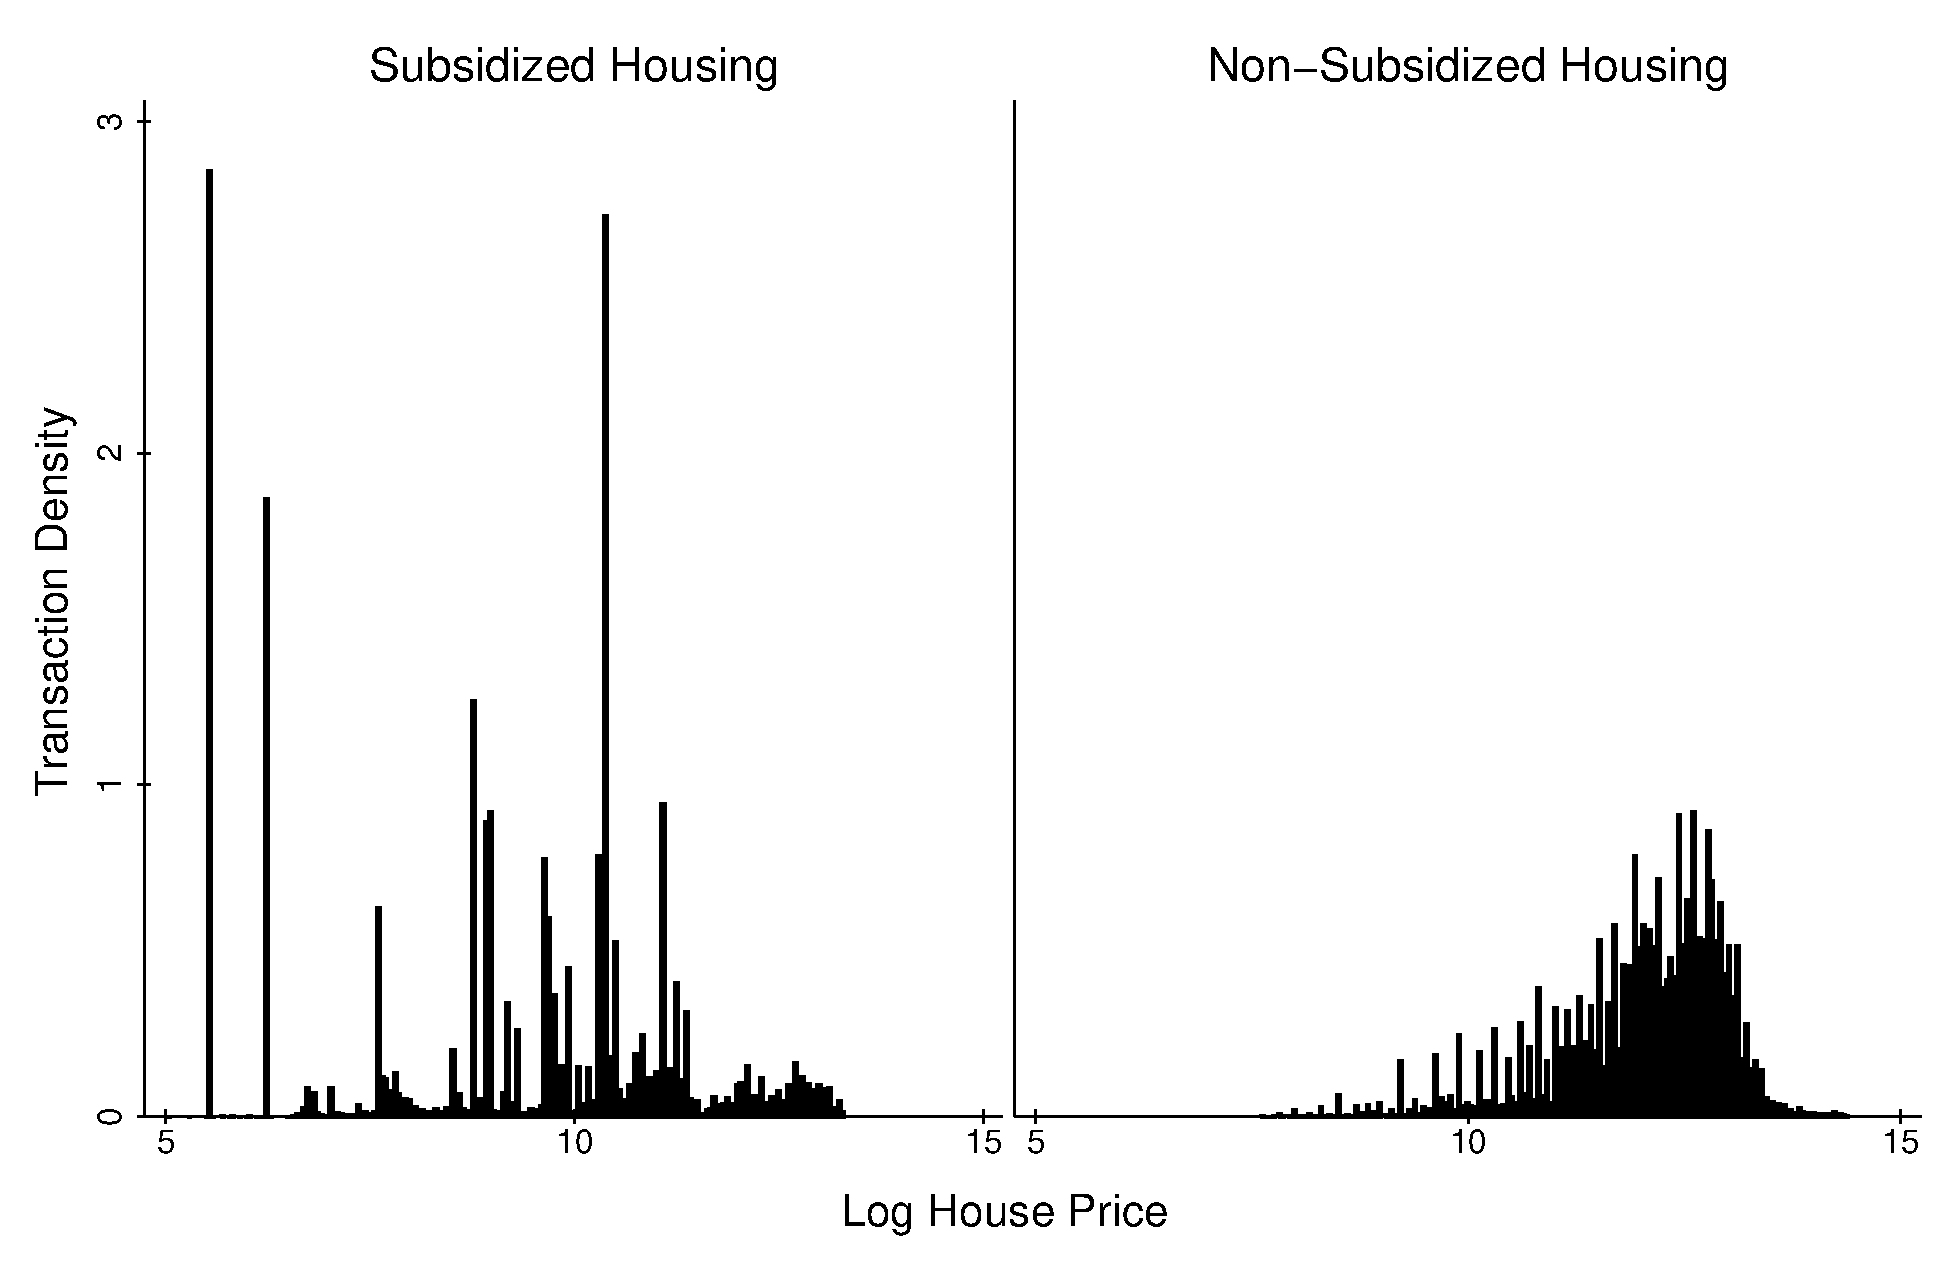
\includegraphics[scale=.4,trim={0cm 0cm -1cm 0cm}]{figures/summary_pricedist.pdf}
\\
\footnotesize{Note: Transactions are censored at R100,000.}
\end{figure}


\begin{figure}[h!]
\centering
\caption{Housing Transactions relative to Each Project's Modal Transaction Month}
\label{appendix:histfreq}

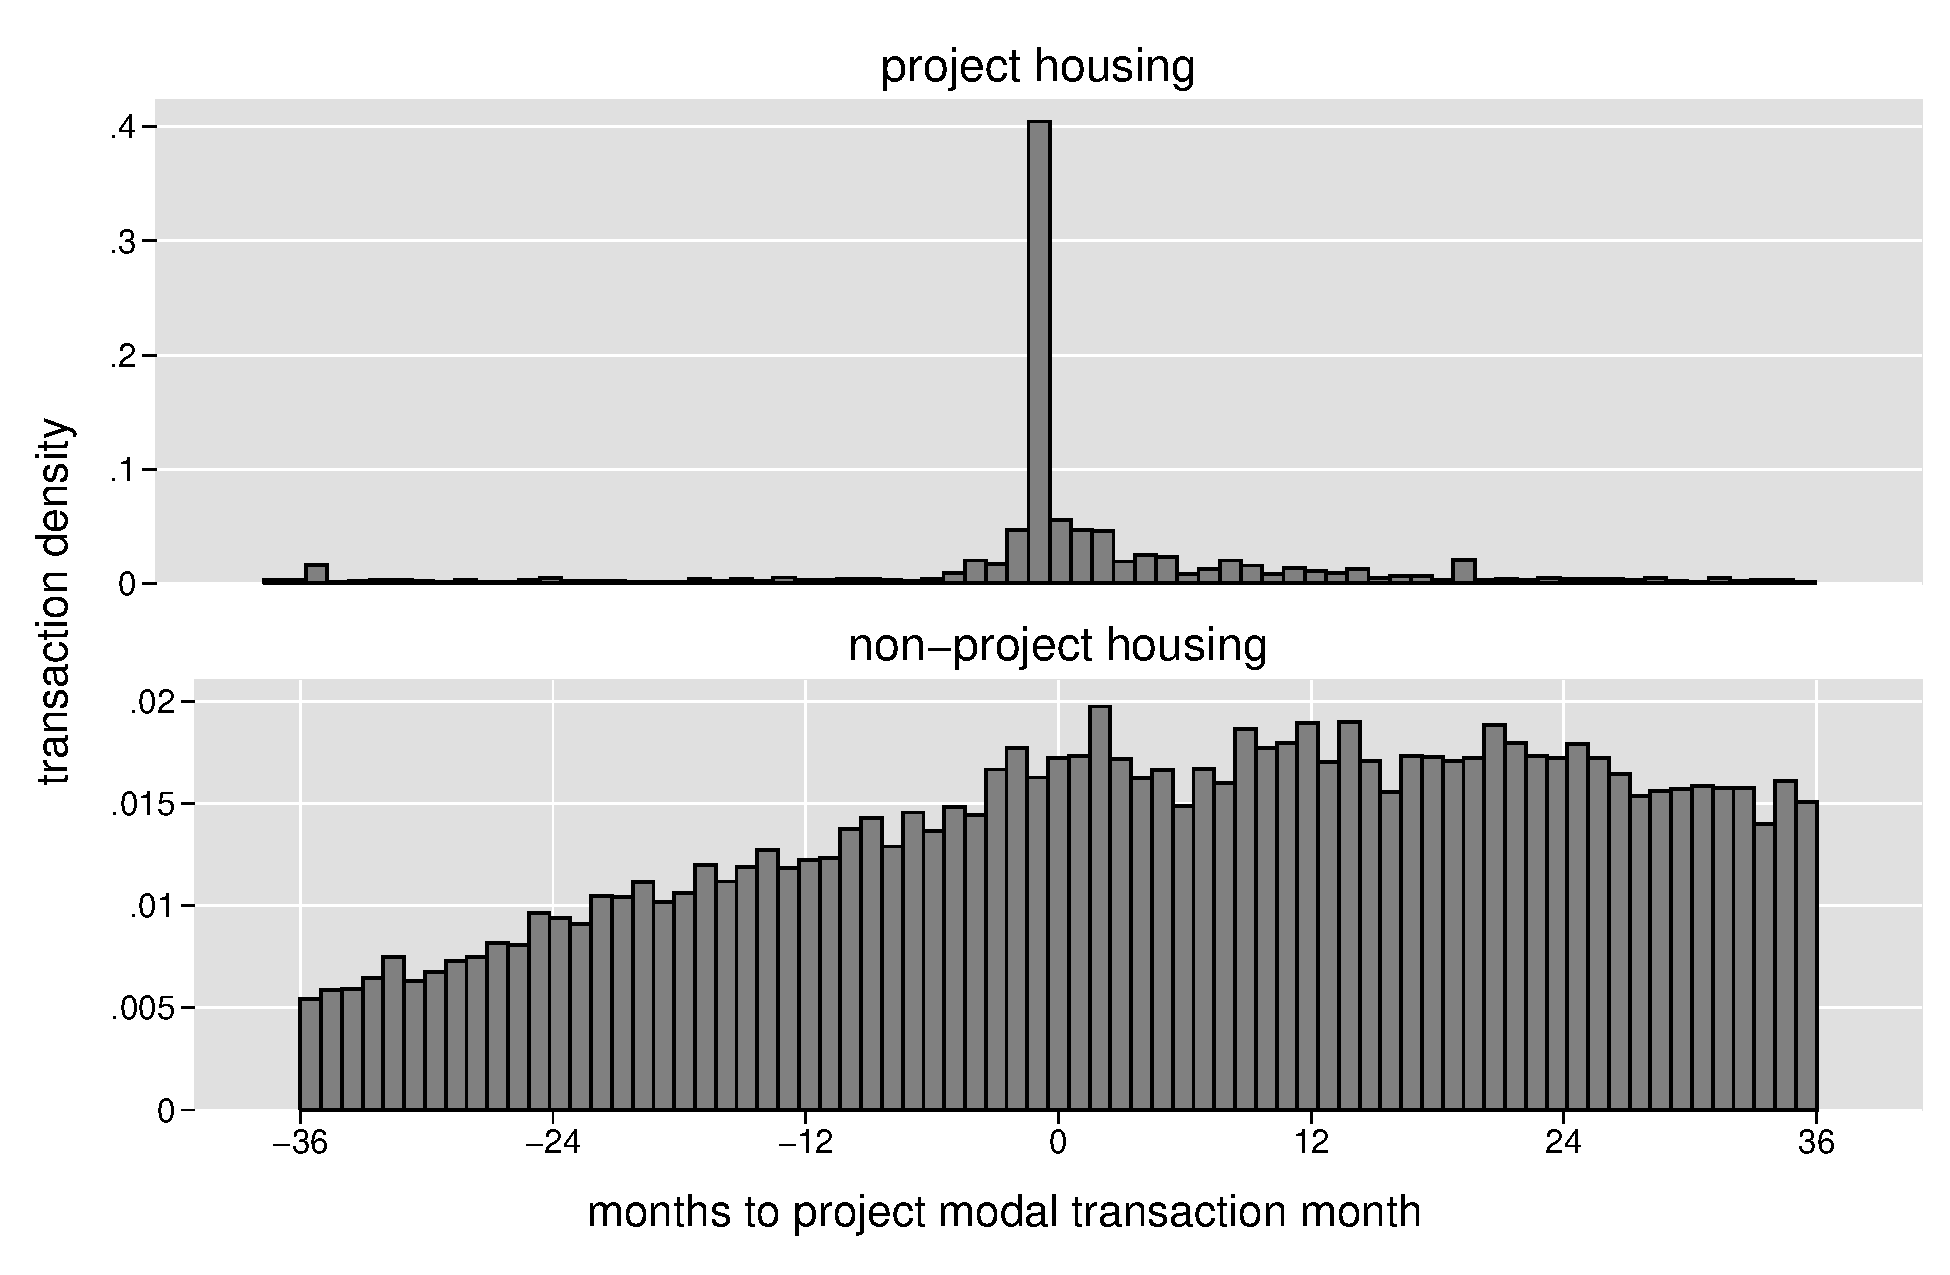
\includegraphics[scale=.4 , trim={.2cm 0.2cm .2cm 0.2cm},clip]{figures/summary_densitytime.pdf}

\end{figure}


\begin{table}[ht!]
\centering
\caption{Project Descriptions}\label{table:projectdescriptions}
\vspace{-2mm}
\begin{tabular}{l*{1}{c}}
\toprule
 &Counts  \\
\midrule
\textbf{Constructed} & \\[.5em]
current  & 89 \\current/overflow  & 24 \\under implementation  & 45 \\complete  & 14 \\[.5em]
Total constructed  & 172 \\[.5em]
\textbf{Unconstructed} & \\[.5em]
proposed  & 71 \\under planning  & 40 \\future  & 16 \\investigating  & 10 \\uncertain  & 8 \\[.5em]
Total unconstructed  & 145 \\[.5em]
\textbf{Other} \\[.5em]
informal  & 87 \\hostel  & 23 \\new  & 27 \\upg  & 6 \\p  & 1 \\no description  & 181 \\[.5em]
Total other  & 325 \\[.5em]
\midrule
Total  & 642 \\[.5em]
\bottomrule
\end{tabular}
\end{table}



\subsection{String Matching for Project Names and Delivery Dates }
\label{appendix:stringmatch}


We then use a fuzzy-string matching algorithm with bigrams to link project names from the budget reports to the administrative maps.  We keep all matches with over 60\% similarity, with 37 projects matching exactly.  Appendix~\ref{table:stringmatch} compares unmatched and matched projects finding that matched projects have much higher numbers of project houses, lower nearby housing prices, and are further from the central business district compared to unmatched projects.  One reason may be that the budget reports only include larger, more expansive projects, which are likely to take place further from city centers. 


\vspace{0mm}
\begin{table}[h!]
\centering
\caption{Assessing Name Matching between Budget Reports and Administrative Project Records}\label{table:stringmatch}
\vspace{0mm}
\begin{tabular}{l*{1}{cccc}}
\toprule
  & \multicolumn{2}{c}{\textbf{Matched}}& \multicolumn{2}{c}{\textbf{Unmatched}}    \\
  &Const. & Unconst. &Const. & Unconst.  \\
\midrule
 Number of Projects  & 126  & 73  & 46  & 72  \\ 
 Area (km2)  & 1.22  & 1.02  & 1.05  & 1.30  \\ 
 Delivered Houses  & 416  & 15  & 259  & 7  \\ 
 House Price in 1 km (R$^\dagger$)  & 183,930  & 206,496  & 199,923  & 232,166  \\ 
 Distance to CBD$^\ddagger$ (km)  & 34.3  & 31.3  & 27.5  & 24.0  \\ 

\bottomrule
\multicolumn{5}{l}{\scriptsize Const. refers to constructed projects and unconst. refers to unconstructed projects.}\\[-.5em]
\multicolumn{5}{l}{\scriptsize $^*$Calculated from {\it expected} completion dates using Gauteng National Treasury budget reports.}\\[-.5em]
\multicolumn{5}{l}{\scriptsize $^\dagger$ The USD averaged to about 7.70 Rands during the 2001-2011 period.}\\[-.5em]
\multicolumn{5}{l}{\scriptsize $^\ddagger$Measured as the average minimum distance with respect to Johannesburg and Pretoria CBDs. } \\[-.5em]
\end{tabular}
\end{table} 





% \subsection{Project counts}
% \label{appendix:projectcounts}
% \vspace{-5mm}
% \begin{figure}[ht!]
% \centering
% 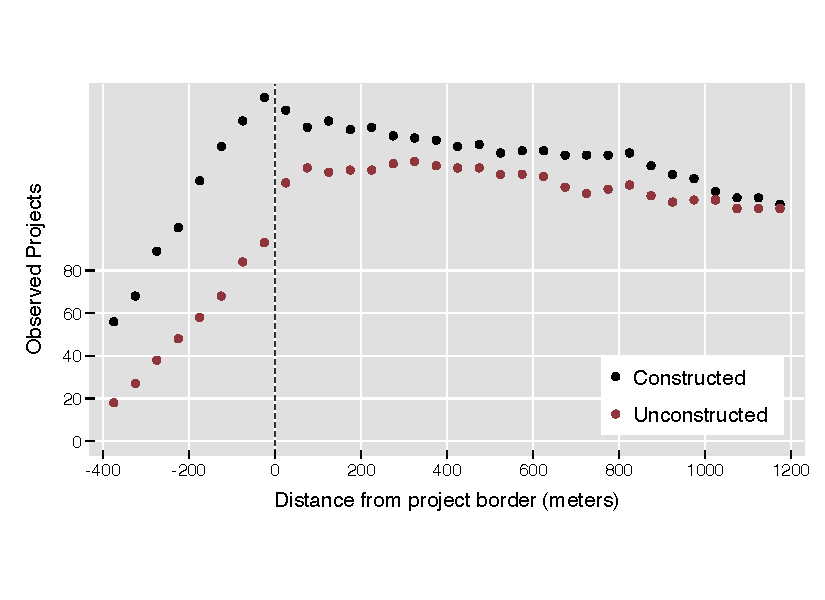
\includegraphics[scale=1.2,trim={.1cm 1.2cm .1cm 1.2cm},clip]{figures/projectcounts_4.pdf}
% \end{figure}



\begin{table}[h!]
	\centering
	\caption{Mean Census Characteristics in the Pre-Period}\label{table:projectdescriptivescensus}
\vspace{-2mm}
\begin{threeparttable}
\begin{tabular}{l*{1}{ccc}}
\toprule
& Constructed & Unconstructed & All Census Blocks \\
\midrule
Flush Toilet&0.86&0.68&0.82 \\
Piped Water in Home&0.48&0.20&0.42 \\
Electricity for Cooking&0.79&0.42&0.71 \\
Electricity for Heating&0.76&0.37&0.68 \\
Electricity for Lighting&0.85&0.63&0.80 \\
Number of Rooms&3.69&2.81&3.51 \\
Household Size&3.48&3.44&3.47 \\
\% Area Overlap with Projects&0.97&0.89&0.65 \\
N&          5,391&          1,400&          6,834 \\
 
\bottomrule
\end{tabular}
\begin{tablenotes}
\item \footnotesize Data are from the 1996 and 2001 Censuses of Population and Housing.
``Constructed'' and ``Unconstructed'' include census blocks with over 50\% 
 area overlap with constructed and unconstructed projects. 
``All''  includes all blocks.  Means are weighted by land area.
\end{tablenotes}
\end{threeparttable}
\end{table}


\begin{table}[hbt!]
\small
\centering
\caption{Housing Density Estimates by Distances Outside Projects}\label{table:bbluDDDdist}
\vspace{-2mm}
\resizebox{1\linewidth}{!}{
\begin{threeparttable}
\begin{tabular}{lCCCCC}
\toprule
& \small (1) & \small (2) & \small (3) & \small (4) & \small (5) \\
 & \small Total Housing & \small Formal Housing & \small Informal Housing & \small Informal Backyard Housing & \small Informal Non-Bkyd. Housing \\ \midrule
\textsc{0-500m}     &      -187.0\textsuperscript{c}&       -22.4                   &      -164.6\textsuperscript{c}&       -75.6                   &       -89.0                   \\
                    &     (110.1)                   &      (61.6)                   &      (92.6)                   &      (80.9)                   &      (80.2)                   \\[0.55em]
\textsc{500-750m}   &        28.0                   &        18.8                   &         9.2                   &       -11.5                   &        20.7                   \\
                    &      (36.5)                   &      (17.0)                   &      (29.1)                   &      (14.9)                   &      (24.6)                   \\[0.55em]
\textsc{750-1000m}  &        72.3\textsuperscript{b}&        26.3\textsuperscript{b}&        46.0\textsuperscript{c}&        14.5                   &        31.5                   \\
                    &      (30.1)                   &      (11.7)                   &      (25.1)                   &      (14.3)                   &      (20.1)                   \\[0.55em]
Mean Pre            &      579.36                   &      288.49                   &      290.87                   &      184.19                   &      106.68                   \\
Mean Post           &      922.93                   &      424.41                   &      498.52                   &      182.46                   &      316.06                   \\
R$^2$               &       0.322                   &       0.292                   &       0.276                   &       0.272                   &       0.200                   \\
N                   &   6,143,756                   &   6,143,756                   &   6,143,756                   &   6,143,756                   &   6,143,756                   \\

\bottomrule
\end{tabular}
\begin{tablenotes}
\item \footnotesize Coefficients capture the interactions of \textsc{Post}$\times$\textsc{Constructed} at 0-500m, 500-750m, and 750-1000m where the control distance group is 1000-1500m.  Standard errors clustered at the project level are in parenthesis. \textsuperscript{c} p$<$0.10,\textsuperscript{b} p$<$0.05,\textsuperscript{a} p$<$0.01 \,\,
Project areas are 25m by 25m plots within 1,500m of project footprints.
Estimates control for 2001 census sub-place fixed effects.
Housing densities are measure in terms of houses per $\text{km}^{2}$.
% ``inside'' means within project footprint.  ``constr'' means constructed.
\end{tablenotes}
\end{threeparttable}
}
\end{table}



\begin{table}[hbt!]
\small
\centering
\caption{Full Census Estimates}\label{table:censusestimatesfull}
\vspace{-2mm}
% \resizebox{1\linewidth}{!}{
\begin{threeparttable}
\begin{tabular}{lDDDDD}
\toprule
 & \small (1) & \small (2)  & \small (3) & \small (4) & \small (5) \\
& \small Has Piped Water Indoors  & \small Has a Flush Toilet  & \small Has Electricity & \small Total Rooms &  \small People per $\text{km}^{2}$   \\ \midrule
inside $\times$ constr $\times$ post&       0.298\textsuperscript{b}&       0.063                   &      -0.143                   &      -0.031                   &    2584.083\textsuperscript{b}\\
                    &     (0.132)                   &     (0.185)                   &     (0.239)                   &     (1.577)                   &  (1278.139)                   \\[0.01em]
0-500m away $\times$ constr $\times$ post&       0.025                   &      -0.115                   &      -0.074                   &      -0.145                   &     175.090                   \\
                    &     (0.092)                   &     (0.080)                   &     (0.089)                   &     (0.397)                   &   (736.878)                   \\[0.05em]
inside $\times$ post&      -0.114                   &       0.193                   &       0.325                   &       0.441                   &     550.823                   \\
                    &     (0.110)                   &     (0.169)                   &     (0.229)                   &     (1.556)                   &  (1169.822)                   \\[0.01em]
0-500m away $\times$ post&      -0.029                   &       0.081                   &       0.099                   &       0.054                   &    1357.945\textsuperscript{b}\\
                    &     (0.084)                   &     (0.067)                   &     (0.081)                   &     (0.365)                   &   (670.812)                   \\[0.05em]
constr $\times$ post&       0.067\textsuperscript{c}&       0.106\textsuperscript{a}&       0.051                   &       0.164                   &    -286.022                   \\
                    &     (0.040)                   &     (0.038)                   &     (0.038)                   &     (0.172)                   &   (177.846)                   \\[0.5em]
inside $\times$ constr&       0.129                   &      -0.022                   &      -0.103                   &      -0.378                   &    2740.110\textsuperscript{a}\\
                    &     (0.094)                   &     (0.121)                   &     (0.114)                   &     (0.608)                   &   (642.330)                   \\[0.01em]
0-500m away $\times$ constr&       0.009                   &       0.080                   &       0.035                   &       0.038                   &    1055.727\textsuperscript{c}\\
                    &     (0.082)                   &     (0.075)                   &     (0.078)                   &     (0.332)                   &   (623.427)                   \\[0.05em]
post                &       0.057\textsuperscript{b}&       0.008                   &       0.055\textsuperscript{b}&       0.305\textsuperscript{b}&     620.190\textsuperscript{a}\\
                    &     (0.027)                   &     (0.024)                   &     (0.025)                   &     (0.126)                   &   (124.934)                   \\
inside              &      -0.279\textsuperscript{a}&      -0.088                   &      -0.061                   &      -0.110                   &    -581.279                   \\
                    &     (0.086)                   &     (0.110)                   &     (0.102)                   &     (0.609)                   &   (464.306)                   \\[0.01em]
0-500m away         &      -0.018                   &      -0.025                   &      -0.031                   &       0.032                   &     722.742                   \\
                    &     (0.075)                   &     (0.065)                   &     (0.072)                   &     (0.294)                   &   (581.744)                   \\[0.01em]
constr              &      -0.089\textsuperscript{b}&      -0.125\textsuperscript{b}&      -0.061                   &      -0.425\textsuperscript{b}&    -164.079                   \\
                    &     (0.044)                   &     (0.049)                   &     (0.040)                   &     (0.202)                   &   (168.959)                   \\[0.1em]
Mean Pre            &        0.47                   &        0.71                   &        0.70                   &        3.48                   &    1,793.45                   \\
Mean Post           &        0.54                   &        0.77                   &        0.77                   &        3.79                   &    2,690.42                   \\
R$^2$               &       0.577                   &       0.612                   &       0.574                   &       0.587                   &       0.551                   \\
N                   &      20,639                   &      20,639                   &      20,639                   &      20,500                   &      21,197                   \\
 
% project{\tim}post{\tim}constr&       0.115\textsuperscript{c}&       0.164\textsuperscript{a}&       0.259\textsuperscript{a}&       0.181\textsuperscript{a}&       0.066                   &      -0.074                   &      -0.266\textsuperscript{b}&      99.563                   \\
            &     (0.069)                   &     (0.050)                   &     (0.072)                   &     (0.066)                   &     (0.084)                   &     (0.173)                   &     (0.107)                   &  (1448.879)                   \\[0.5em]
project{\tim}post&       0.064                   &       0.090\textsuperscript{b}&       0.176\textsuperscript{a}&       0.151\textsuperscript{a}&       0.144\textsuperscript{b}&       0.408\textsuperscript{a}&      -0.039                   &    2320.431\textsuperscript{b}\\
            &     (0.046)                   &     (0.039)                   &     (0.060)                   &     (0.055)                   &     (0.066)                   &     (0.129)                   &     (0.056)                   &  (1111.722)                   \\[0.5em]
project{\tim}constr&       0.070                   &      -0.024                   &      -0.066                   &      -0.061                   &       0.129                   &       0.195                   &       0.460\textsuperscript{a}&    -611.013                   \\
            &     (0.111)                   &     (0.090)                   &     (0.105)                   &     (0.093)                   &     (0.125)                   &     (0.284)                   &     (0.128)                   &  (1733.494)                   \\[0.5em]
project     &      -0.321\textsuperscript{a}&      -0.239\textsuperscript{a}&      -0.354\textsuperscript{a}&      -0.320\textsuperscript{a}&      -0.362\textsuperscript{a}&      -1.065\textsuperscript{a}&      -0.403\textsuperscript{a}&     416.265                   \\
            &     (0.077)                   &     (0.053)                   &     (0.069)                   &     (0.064)                   &     (0.080)                   &     (0.175)                   &     (0.082)                   &   (691.463)                   \\[0.5em]
spillover{\tim}post{\tim}constr&       0.013                   &       0.045                   &       0.028                   &      -0.037                   &      -0.038                   &       0.053                   &      -0.153\textsuperscript{a}&     444.064                   \\
            &     (0.034)                   &     (0.033)                   &     (0.034)                   &     (0.043)                   &     (0.027)                   &     (0.078)                   &     (0.049)                   &   (470.258)                   \\[0.5em]
spillover{\tim}post&       0.039                   &       0.133\textsuperscript{a}&       0.101\textsuperscript{a}&       0.082\textsuperscript{a}&       0.058\textsuperscript{b}&       0.249\textsuperscript{a}&      -0.156\textsuperscript{a}&     652.913\textsuperscript{b}\\
            &     (0.024)                   &     (0.028)                   &     (0.024)                   &     (0.023)                   &     (0.023)                   &     (0.055)                   &     (0.036)                   &   (325.594)                   \\[0.5em]
spillover{\tim}constr&      -0.029                   &      -0.056                   &      -0.065                   &      -0.041                   &       0.015                   &      -0.252\textsuperscript{c}&       0.143\textsuperscript{b}&     -23.442                   \\
            &     (0.049)                   &     (0.055)                   &     (0.044)                   &     (0.042)                   &     (0.050)                   &     (0.145)                   &     (0.059)                   &  (1353.816)                   \\ \midrule
{\it p}-val, h\textsubscript{0}: project=spill. &       0.119                   &       0.029                   &       0.001                   &       0.001                   &       0.208                   &       0.439                   &       0.250                   &       0.811                   \\
Mean Outcome 2001&        0.72                   &        0.31                   &        0.60                   &        0.57                   &        0.75                   &        3.31                   &        3.59                   &    7,313.26                   \\
Mean Outcome 2011&        0.79                   &        0.51                   &        0.80                   &        0.69                   &        0.82                   &        3.57                   &        3.22                   &    9,118.36                   \\
R$^2$       &       0.336                   &       0.318                   &       0.363                   &       0.315                   &       0.294                   &       0.368                   &       0.443                   &       0.398                   \\
\# projects &         117                   &         117                   &         117                   &         117                   &         117                   &         117                   &         117                   &         117                   \\
N project areas&       3,631                   &       3,631                   &       3,631                   &       3,631                   &       3,631                   &       3,630                   &       3,632                   &       3,632                   \\
N spillover areas&       5,978                   &       5,978                   &       5,978                   &       5,978                   &       5,978                   &       5,964                   &       5,977                   &       5,980                   \\
N           &       9,609                   &       9,609                   &       9,609                   &       9,609                   &       9,609                   &       9,594                   &       9,609                   &       9,612                   \\

\bottomrule
\end{tabular}
\begin{tablenotes}
\item Standard errors clustered at the project level in parenthesis.\textsuperscript{c} p$<$0.10,\textsuperscript{b} p$<$0.05,\textsuperscript{a} p$<$0.01
Outcomes in Columns (1), (2), and (3) are indicator variables.
Specifications include census 2001 subplace fixed effects.
Results are weighted by unit area and control for up to a cubic in unit area by time. 
``HH'' stands for household.
\end{tablenotes}
\end{threeparttable}
% }
\end{table}



\begin{table}[hbt!]
\small
\centering
\caption{Census Demographic  Estimates}\label{table:censusestimatesfull2}
\vspace{-2mm}
\resizebox{1\linewidth}{!}{
\begin{threeparttable}
\begin{tabular}{lDDDDD}
\toprule
 & \small (1) & \small (2)  & \small (3)  & \small (4) & \small (5)   \\
 & \small HH Size & Age HoH & HoH is African  & HoH is Employed  & HH Log Income \\ \midrule
inside $\times$ constr $\times$ post&       0.840\textsuperscript{a}&      -1.120                   &       0.071                   &       0.009                   &       0.048                   \\
                    &     (0.323)                   &     (3.876)                   &     (0.087)                   &     (0.113)                   &     (0.304)                   \\[0.01em]
0-500m away $\times$ constr $\times$ post&       0.169                   &      -0.410                   &      -0.006                   &      -0.011                   &       0.142                   \\
                    &     (0.184)                   &     (1.416)                   &     (0.066)                   &     (0.040)                   &     (0.170)                   \\[0.05em]
inside $\times$ post&      -0.430                   &       1.162                   &      -0.063                   &       0.008                   &      -0.270                   \\
                    &     (0.272)                   &     (3.805)                   &     (0.081)                   &     (0.110)                   &     (0.269)                   \\[0.01em]
0-500m away $\times$ post&       0.030                   &       0.869                   &       0.013                   &       0.037                   &      -0.380\textsuperscript{b}\\
                    &     (0.167)                   &     (1.317)                   &     (0.058)                   &     (0.037)                   &     (0.155)                   \\[0.05em]
constr $\times$ post&      -0.177\textsuperscript{b}&       0.344                   &      -0.055                   &       0.032\textsuperscript{c}&      -0.092                   \\
                    &     (0.076)                   &     (0.551)                   &     (0.036)                   &     (0.018)                   &     (0.082)                   \\[0.5em]
inside $\times$ constr&       0.139                   &      -0.332                   &      -0.169\textsuperscript{b}&       0.085                   &       0.346                   \\
                    &     (0.239)                   &     (1.655)                   &     (0.073)                   &     (0.073)                   &     (0.218)                   \\[0.01em]
0-500m away $\times$ constr&       0.040                   &       1.306                   &      -0.028                   &       0.018                   &      -0.063                   \\
                    &     (0.160)                   &     (1.029)                   &     (0.065)                   &     (0.030)                   &     (0.124)                   \\[0.05em]
post                &      -0.257\textsuperscript{a}&       0.988\textsuperscript{a}&       0.095\textsuperscript{a}&       0.021\textsuperscript{b}&       1.112\textsuperscript{a}\\
                    &     (0.054)                   &     (0.370)                   &     (0.023)                   &     (0.010)                   &     (0.063)                   \\
inside              &      -0.188                   &      -0.274                   &       0.263\textsuperscript{a}&      -0.157\textsuperscript{b}&      -0.558\textsuperscript{a}\\
                    &     (0.206)                   &     (1.601)                   &     (0.065)                   &     (0.072)                   &     (0.213)                   \\[0.01em]
0-500m away         &       0.020                   &      -1.158                   &       0.041                   &      -0.053\textsuperscript{c}&       0.103                   \\
                    &     (0.151)                   &     (0.929)                   &     (0.054)                   &     (0.029)                   &     (0.114)                   \\[0.01em]
constr              &      -0.077                   &      -0.841                   &       0.097\textsuperscript{b}&      -0.024\textsuperscript{c}&      -0.136\textsuperscript{c}\\
                    &     (0.076)                   &     (0.546)                   &     (0.047)                   &     (0.014)                   &     (0.075)                   \\[0.1em]
Mean Pre            &        3.25                   &       41.26                   &        0.73                   &        0.82                   &        7.30                   \\
Mean Post           &        2.89                   &       42.34                   &        0.81                   &        0.83                   &        8.25                   \\
R$^2$               &       0.703                   &       0.579                   &       0.721                   &       0.573                   &       0.746                   \\
N                   &      20,509                   &      20,505                   &      20,641                   &      20,501                   &      20,495                   \\

\bottomrule
\end{tabular}
\begin{tablenotes}
\item \footnotesize Standard errors clustered at the project level in parenthesis.\textsuperscript{c} p$<$0.10,\textsuperscript{b} p$<$0.05,\textsuperscript{a} p$<$0.01 \,\,
Outcomes in Columns (4) and (5) are indicator variables.
Specifications include census 2001 subplace fixed effects.
Results are weighted by unit area and control for up to a cubic polynomial in unit area by time.  ``HH'' stands for household and ``HoH'' stands for head of household.
\end{tablenotes}
\end{threeparttable}
}
\end{table}




\begin{table}[hbt!]
\centering
\caption{Full Housing Demand Estimates}\label{table:housingdemandestimates_full}
\vspace{-2mm}
\resizebox*{!}{.97\textheight}{
\begin{threeparttable}
\begin{tabular}{lDD}
\toprule
 &  Formal &  Informal \\ \midrule 
 Net Amenities: $\overline{V} = ( \overline{\delta}_{hl} - \theta \overline{C}_{hlt} )$ \\[.5em]
\textsc{Proj} $\times$ \textsc{Constr} $\times$ \textsc{Post} &        0.32\textsuperscript{c}&       -0.19\textsuperscript{c}\\
                    &      (0.19)                   &      (0.10)                   \\
\textsc{Spill}  $\times$ \textsc{Constr}  $\times$ \textsc{Post} &       -0.02                   &       -0.12                   \\
                    &      (0.07)                   &      (0.09)                   \\
\textsc{Proj} $\times$ \textsc{Post} &        0.50\textsuperscript{a}&        0.15                   \\
                    &      (0.16)                   &      (0.09)                   \\
\textsc{Spill}  $\times$ \textsc{Post} &        0.16\textsuperscript{b}&        0.10                   \\
                    &      (0.06)                   &      (0.09)                   \\
\textsc{Constr} $\times$ \textsc{Post} &       -0.02                   &       -0.02                   \\
                    &      (0.02)                   &      (0.04)                   \\
\textsc{Proj} $\times$ \textsc{Constr}&        0.48\textsuperscript{b}&        0.35                   \\
                    &      (0.20)                   &      (0.21)                   \\
\textsc{Spill} $\times$ \textsc{Constr}&       -0.26\textsuperscript{c}&       -0.19                   \\
                    &      (0.15)                   &      (0.17)                   \\
\textsc{Post}       &        0.08\textsuperscript{a}&        0.22\textsuperscript{a}\\
                    &      (0.02)                   &      (0.03)                   \\
\textsc{Proj}       &       -0.73\textsuperscript{a}&        0.43\textsuperscript{b}\\
                    &      (0.16)                   &      (0.17)                   \\
\textsc{Spill}      &        0.35\textsuperscript{a}&        0.57\textsuperscript{a}\\
                    &      (0.12)                   &      (0.14)                   \\
\textsc{Constr}     &        0.31\textsuperscript{a}&        0.30\textsuperscript{a}\\
                    &      (0.10)                   &      (0.10)                   \\
[.3em]
  Marginal Utility of Income: $ -\theta $  &  -0.0000165\textsuperscript{a}&  -0.0000180\textsuperscript{a}\\
                    & (0.0000062)                   & (0.0000067)                   \\
[.5em]
cut point: $\Lambda_{h}(1)$&      -0.815                   &      -0.580                   \\
                    &     (0.834)                   &     (0.902)                   \\

Cut Point: $\Lambda_{h}(2)$&      -0.428                   &      -0.321                   \\
                    &     (0.838)                   &     (0.901)                   \\

Cut Point: $\Lambda_{h}(3)$&       0.284                   &      -0.060                   \\
                    &     (0.837)                   &     (0.900)                   \\

cut point: $\Lambda_{h}(4)$&       0.797                   &       0.158                   \\
                    &     (0.837)                   &     (0.900)                   \\

cut point: $\Lambda_{h}(5)$&       1.270                   &       0.365                   \\
                    &     (0.836)                   &     (0.899)                   \\

arctan correlation of amenity shocks &       0.725\textsuperscript{a}\\
                    &     (0.030)                   \\
N                   &   6,143,756                   \\

Cut Point: $\Lambda_{h}(7)$&       1.887\textsuperscript{b}&       0.683                   \\
                    &     (0.830)                   &     (0.897)                   \\

Cut Point: $\Lambda_{h}(8)$&       1.998\textsuperscript{b}&       0.802                   \\
                    &     (0.828)                   &     (0.897)                   \\

cut point: $\Lambda_{h}(9)$&       2.245\textsuperscript{a}&       0.947                   \\
                    &     (0.823)                   &     (0.897)                   \\

Cut Point: $\Lambda_{h}(10)$&       2.320\textsuperscript{a}&       1.045                   \\
                    &     (0.822)                   &     (0.898)                   \\
[.3em]
% arctan correlation of amenity shocks &       0.725\textsuperscript{a}\\
                    &     (0.030)                   \\
N                   &   6,143,756                   \\

Correlation of amenity shocks: $\rho_{for,inf}$ & $0.620^{\text{a}}$ & \\
 & (0.018) & \\[.3em]
 N & 6,143,756 & \\
\bottomrule
% \\[-.6em]
% \multicolumn{3}{l}{ \footnotesize Standard errors clustered at the project level in parenthesis. \textsuperscript{c} p$<$0.10,\textsuperscript{b} p$<$0.05,\textsuperscript{a} p$<$0.01 } \\[-.3em]
% \multicolumn{3}{l}{ \footnotesize Outcome categories by plot and year include categories for formal and informal} \\[-.3em]
% \multicolumn{3}{l}{ \footnotesize  building counts from 0 to 9 and a category at least 10.  Table~\ref{table:housingdemandestimates_full} includes the full set} \\[-.3em]
% \multicolumn{3}{l}{ \footnotesize of coefficients.  Net amenities equal local amenities minus local housing costs. } \\[-.3em]
\end{tabular}
\begin{tablenotes}
\item \footnotesize Standard errors clustered at the project level in parenthesis.  \textsuperscript{c} p$<$0.10,\textsuperscript{b} p$<$0.05,\textsuperscript{a} p$<$0.01  \,\, Outcome categories by plot and year include categories for formal and informal  building counts from 0 to 9 and a category at least 10.  Net amenities equal local amenities minus local housing costs. ``\textsc{Constr}'' refers to ``Constructed.''
\end{tablenotes}
\end{threeparttable}
}
\end{table}


\afterpage{

\subsection{Pre-Trends for Price Estimates}\label{section:appendixpricerobust}

To examine dynamics of price effects especially in terms of pretrends, we estimate effects with respect to months to the (expected) construction month of each project using the following specification:
\begin{align}
\label{eq:pricerobust}
\begin{split}
\quad y_{ipnt} \, =&   \, \beta_1 \, \textsc{\small Spill}_{i}\times\textsc{\small Const}_{p} \, + \, \beta_2 \, \textsc{\small Spill}_{i} \, + \, \beta_3 \, \textsc{\small Const}_{p}\,  \\
 &\, + \sum_{l=1}^{9} T_{l} \, \Big( \, \alpha_1^{l} \, \textsc{\small Spill}_{i}\times\textsc{\small Const}_{p} \, + \, \alpha_2^{l} \, \textsc{\small Spill}_{i} \, + \, \alpha_3^{l} \, \textsc{\small Const}_{p}\, +\, \alpha_4^{l} \Big) \,  \\
&\, + \, \theta \, X_{ipnt} \, + \, \lambda_n \, + \, \varepsilon_{ipnt} \quad \\
\text{Where }& \\
&T_1 = \mathbbm{1} \Big\{\, t \leq -48  \,\Big\} \,, \,\,\, T_2 = \mathbbm{1} \Big\{ -48 \leq t < -36 \Big\} \,, \,\,\, T_3 = \mathbbm{1} \Big\{ -36 \leq t < -24 \Big\} \,\,, \\
&T_4 = \mathbbm{1}  \Big\{ -24 \leq t < -12 \Big\} \,, \,\,\, T_5 = \mathbbm{1} \Big\{ 0 \leq t < 12 \Big\} \,, \,\,\, T_6 = \mathbbm{1} \Big\{ 12 \leq t < 24 \Big\} \,\,, \\
&T_7 = \mathbbm{1} \Big\{ 24< t<=36 \Big\} \,\, ,\,\,T_8\,=\,\mathbbm{1} \Big\{ 36< t <=48 \Big\} \, , \,\,\, T_9 = \mathbbm{1} \Big\{ 48 \leq t \Big\} 
\end{split}
\end{align}
\noindent where $\textsc{\small Spill}_{i}$ is an indicator for properties within 500 meters outside of a project boundary and $\textsc{\small Const}_{p}$ is an indicator for being nearby a project that is successfully constructed.  $t$ indexes months to scheduled construction with the scheduled construction month normalized to zero.  Differential prices near and far from constructed projects compared to unconstructed projects are estimated separately according to years to scheduled construction relative to the year before scheduled construction.  This specification leaves transactions occurring in the 12 months immediately before scheduled construction as the omitted category.  Coefficient, $\beta_1$ captures differential changes in log-prices near and far from constructed and unconstructed projects across all time periods.  The coefficients of interest, $\alpha_1^{l}$ track how prices change differentially in the 9 time windows relative to the omitted category --- 12 months before scheduled construction.  Additional controls $X_{ipnt}$ include up to a cubic polynomial in the lot size of properties as well as a fixed effects for the year-month of each transaction.  The specification also includes neighborhood fixed effects $\lambda_n$.  

As a robustness exercise, we also estimate a differences-in-differences specification that compares transactions before and after scheduled construction near and far from projects.  This specification is equal to equation (\ref{eq:pricerobust}) omitting terms with $\textsc{\small Const}_{p}$.  

\begin{table}[h]
\small
\centering
\caption{Log-Price Estimates 0 to 500 Meters Outside of Housing Projects According to Time to Scheduled Construction }\label{table:pricerobust}
\vspace{-1mm}
\begin{threeparttable}
\begin{tabular}{lCCCC}
\toprule
 & \small (1) & \small (2) & \small (3) & \small (4)   \\ 
  & \small Triple Diff & \small Triple Diff &\small Diff-in-Diff & \small Diff-in-Diff \\ \midrule 
 Pre over 4 yrs      &      -0.362                   &      -0.368                   &       0.001                   &      -0.008                   \\
                    &     (0.280)                   &     (0.275)                   &     (0.123)                   &     (0.125)                   \\[0.5em]
Pre 4-3 yrs         &       0.194                   &       0.192                   &       0.278\textsuperscript{b}&       0.277\textsuperscript{b}\\
                    &     (0.157)                   &     (0.156)                   &     (0.114)                   &     (0.114)                   \\[0.5em]
Pre 3-2 yrs         &      -0.057                   &      -0.053                   &      -0.079                   &      -0.069                   \\
                    &     (0.132)                   &     (0.126)                   &     (0.110)                   &     (0.106)                   \\[0.5em]
Pre 2-1 yrs         &      -0.155                   &      -0.156                   &      -0.109                   &      -0.108                   \\
                    &     (0.100)                   &     (0.098)                   &     (0.085)                   &     (0.084)                   \\[0.5em]
Post 0-1 yrs        &      -0.080                   &      -0.073                   &      -0.081                   &      -0.078                   \\
                    &     (0.098)                   &     (0.096)                   &     (0.073)                   &     (0.071)                   \\[0.5em]
Post 1-2 yrs        &      -0.064                   &      -0.043                   &      -0.052                   &      -0.047                   \\
                    &     (0.100)                   &     (0.098)                   &     (0.079)                   &     (0.075)                   \\[0.5em]
Post 2-3 yrs        &      -0.255\textsuperscript{b}&      -0.233\textsuperscript{b}&      -0.151\textsuperscript{c}&      -0.140\textsuperscript{c}\\
                    &     (0.104)                   &     (0.097)                   &     (0.078)                   &     (0.072)                   \\[0.5em]
Post 3-4 yrs        &      -0.210\textsuperscript{c}&      -0.205\textsuperscript{c}&      -0.173\textsuperscript{c}&      -0.178\textsuperscript{b}\\
                    &     (0.114)                   &     (0.112)                   &     (0.093)                   &     (0.090)                   \\[0.5em]
Post over 4 yrs     &      -0.138                   &      -0.134                   &      -0.092                   &      -0.093                   \\
                    &     (0.098)                   &     (0.097)                   &     (0.079)                   &     (0.078)                   \\[0.5em]
Year-Month FE       &                               &  \checkmark                   &                               &  \checkmark                   \\
Plot Size (up to cubic polynomial)&                               &  \checkmark                   &                               &  \checkmark                   \\
Diff-in-Diff for Constructed Areas&                               &                               &  \checkmark                   &  \checkmark                   \\
R2                  &        0.49                   &        0.49                   &        0.50                   &        0.50                   \\
N                   &      62,349                   &      62,349                   &      34,839                   &      34,839                   \\
 \bottomrule
\end{tabular}
\begin{tablenotes}
\item \footnotesize Estimates capture differential price effects for properties  0 to 500 meters outside of project boundaries relative to   properties 500 to 1,500 meters from boundaries before and after scheduled construction.  Income quartiles are from average household 2001 incomes in census 2001 subplaces.  All estimates include neighborhood fixed effects.  Standard errors clustered at the project level in parenthesis.\textsuperscript{c} p$<$0.10,\textsuperscript{b} p$<$0.05,\textsuperscript{a} p$<$0.01 
\end{tablenotes}
\end{threeparttable}
\end{table} 

}


\begin{figure}[hbt!]
      {  \centering
   \caption[ Histogram of Buildings per Plot with at least 1 Building ]
    {\small Histogram of Buildings per Plot with at least 1 Building }\label{figure:buildhist} 
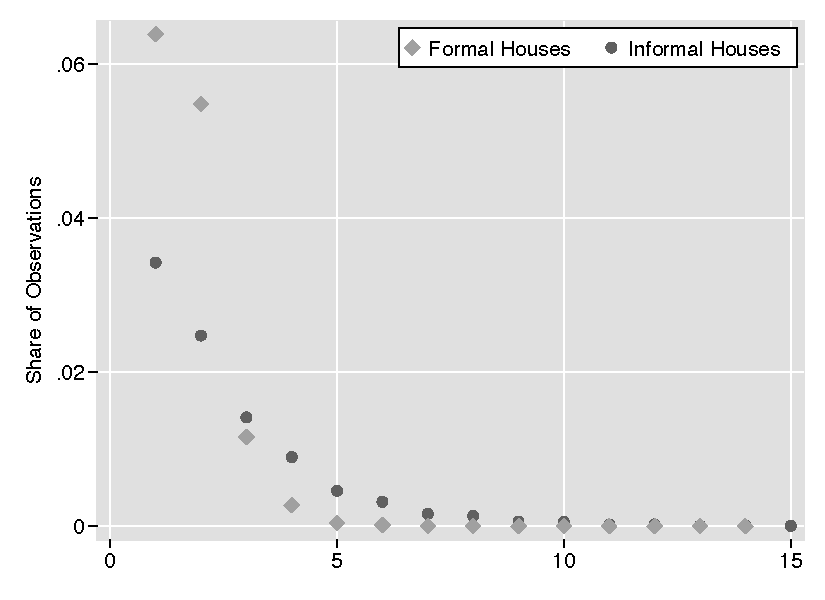
\includegraphics[width=\textwidth,trim={0.3cm .3cm 0.1cm 0cm}, clip=true]{figures/building_hist.pdf}
Plots with zero buildings are not shown.  86\% of plots have zero formal houses, and 91\% of plots have zero informal houses.
This figure also excludes plots with over 15 buildings, which compose less than 0.001\% of the sample.
}
\end{figure}


\afterpage{
\subsection{Full Marginal Probability and Likelihood Function for Demand Estimation}\label{appendix:likelihood}

The probability of observing a given number of formal and informal houses per plot according to equation (\ref{eq:housingdemand}) can be written in terms of a seemingly unrelated bivariate ordered probit model as follows \citep{sajaia2008maximum}
\begin{align}
\label{eq:probfull}
\begin{split}
Pr[ k_{for,jt}^{*} =k_{for} , k_{inf,jt}^{*} =k_{inf} ] \, = \, &  \Phi_2\Bigg(\dfrac{\Lambda_{for}(k_{for}+1) -V_{for,jt} }{\sigma_{for}}, \dfrac{\Lambda_{inf}(k_{inf}+1) - V_{inf,jt}}{\sigma_{inf}} , \rho \Bigg) \\
- \, &\Phi_2\Bigg(\dfrac{\Lambda_{for}(k_{for}) - V_{for,jt} }{\sigma_{for}}, \dfrac{\Lambda_{inf}(k_{inf}+1) - V_{inf,jt} }{\sigma_{inf}} , \rho \Bigg) \\
- \, &\Phi_2\Bigg(\dfrac{\Lambda_{for}(k_{for}+1) - V_{for,jt}}{\sigma_{for}}, \dfrac{\Lambda_{inf}(k_{inf}) - V_{inf,jt}}{\sigma_{inf}} , \rho \Bigg) \\
+ \, &\Phi_2\Bigg(\dfrac{\Lambda_{for}(k_{for}) - V_{for,jt} }{\sigma_{for}}, \dfrac{\Lambda_{inf}(k_{inf}) - V_{inf,jt} }{\sigma_{inf}} , \rho \Bigg) \\
\end{split}
\end{align}
\noindent where $\Phi_{2}(.)$ indicates a standard normal bivariate distribution with correlation terms, $\rho$.  This expression can be estimated by maximizing the following log-likelihood function

The likelihood of observing a given dataset with formal and informal structures on each plot is given by
\begin{align}
\label{eq:demandll}
LL = \sum_{t=1}^{T} \sum_{j=1}^{J} \sum_{m_{for}=1}^{K_{for}} \sum_{m_{inf}=1}^{K_{inf}} \mathbbm{1} \{k_{for,jt} = m_{for}, k_{inf,jt} = m_{inf}\} \,\,\, log \Bigg( Pr[ k_{for,jt}^{*} =k_{for} , k_{inf,jt}^{*} =k_{inf} ] \Bigg)
\end{align}
\noindent where $J$ is the total number of plots observed, $T$ is the total number of time periods, and $K_{for}$ and $K_{inf}$ are the maximum observed number of formal and informal houses observed per plot.  

}

\end{document}


